\documentclass{ucbthesis}
\usepackage{biblatex}



%%%%
\usepackage{syntax} 
\setlength{\grammarparsep}{0.15cm}   % vertical distance between production rules
\setlength{\grammarindent}{1cm}
\renewcommand{\litleft}{\bfseries}
\renewcommand{\ulitleft}{\bfseries}
\newcommand{\superscript}[1]{\ensuremath{^{\textrm{#1}}}}
\newcommand{\subscript}[1]{\ensuremath{_{\textrm{\uppercase{#1}}}}}
\renewcommand{\syntleft}{\normalfont\itshape}
\renewcommand{\syntright}{}
%\newcommand{\deriv}{~::=~}
\newcommand{\deriv}{~ $\rightarrow$ ~}

\usepackage{graphicx}


\usepackage{listings}
\newcommand*{\Comment}[1]{\hfill\makebox[3.0cm][l]{#1}}%
\newcommand*{\BComment}[1]{\Comment{\textbf{#1}}}
\newcommand*{\uncertain}[1]{{\textcolor{red}{\textbf{#1}}}}\newcommand{\sched}[1]{\lstinline[morekeywords={parPre,parPost,recursive,;,||,spawn,join,taskRecursive},mathescape]{#1}}

%\newcommand{\hole}{\fbox{\emph{?hole}}~}
\newcommand{\hole}{{\emph{?hole}}}
%\newcommand{\hlang}{\emph{\texttt{HBOX-AG}}}
%\newcommand{\hlang}{ {\huge \textbf{\textsc{H-AG}}} }
\newcommand{\hlang}{ \texttt{H-AG} }
\newcommand{\hlangpp}{ \texttt{hbox++} }


%%%%


% Double spacing, if you want it.
% \def\dsp{\def\baselinestretch{2.0}\large\normalsize}
% \dsp

% If the Grad. Division insists that the first paragraph of a section
% be indented (like the others), then include this line:
% \usepackage{indentfirst}

\newtheorem{theorem}{Jibberish}

\bibliography{references}

\hyphenation{mar-gin-al-ia}

\begin{document}

% Declarations for Front Matter

\title{Parallelizing the Browser: Synthesis and Optimization of Parallel Tree Traversals}
\author{Leo A. Meyerovich}
\degreesemester{Fall}
\degreeyear{2013}
\degree{Doctor of Philosophy}
\chair{Professor Rastislav Bodik}
\othermembers{Professor George Necula \\
  Professor Krste Asanovic \\
  Professor David Wessel}
\numberofmembers{4}
\prevdegrees{Sc.B. (Brown University) 2007 }
\field{Electrical Engineering and Computer Science}
\campus{Berkeley}

% For a masters thesis, uncomment (remove the % at the beginning of)
% the following line.  This affects the title and approval pages,
% which by default calls this a "dissertation", not a "thesis".

%\itsamasters

% The title page generated by LaTeX is now acceptable for handing in.
% (This was not always the case).

\maketitle
\approvalpage
\copyrightpage

% (This is included by thesis.tex; you do not latex it by itself.)

\begin{abstract}

% The text of the abstract goes here.  If you need to use a \section
% command you will need to use \section*, \subsection*, etc. so that
% you don't get any numbering.  You probably won't be using any of
% these commands in the abstract anyway.

From low-power phones to speed-hungry data visualizations, web browsers need a performance boost. Parallelization is an attractive opportunity because commodity client devices already feature multicore, subword-SIMD, and GPU hardware. However, a typical webpage will not strongly benefit from modern hardware because browsers were only designed for sequential execution. We therefore need to redesign browsers to be parallel. This thesis focuses on a browser component that we found to be particularly challenging to implement: the layout engine. 

We address layout engine implementation by identifying its surprising connection with attribute grammars and then solving key ensuing challenges:
\begin{enumerate}
\item We show how layout engines, both for documents and data visualization, can often be functionally specified in our extended form of attribute grammars. 
\item We introduce a synthesizer that automatically schedules an attribute grammar as a composition of parallel tree traversals. Notably, our synthesizer is fast, simple to extend, and finds schedules that assist aggressive code generation.
\item We make editing parallel code safe by introducing a simple programming construct for partial behavioral specification: schedule sketching. 
\item We optimize tree traversals for SIMD, MIMD, and GPU architectures at tree load time through novel optimizations for data representation and task scheduling.
\end{enumerate}
Put together, we generated a parallel CSS document layout engine that can mostly render complex sites such as Wikipedia. Furthermore, we scripted data visualizations that support interacting with over 100,000 data points in real time.

\end{abstract}


\begin{frontmatter}

\begin{dedication}
\null\vfil
\begin{center}
To You\\\vspace{12pt}
Hey you! out there in the cold 
Getting lonely, getting old, can you feel me 
Hey you! Standing in the aisles 
With itchy feet and fading smiles, can you feel me 
Hey you! don't help them to bury the live 
Don't give in without a fight. 
\end{center}
\vfil\null
\end{dedication}

\tableofcontents
\clearpage
\listoffigures
\clearpage
\listoftables

\begin{acknowledgements}
I want to thank my advisor for advising me.
\end{acknowledgements}

\end{frontmatter}

\pagestyle{headings}

% (Optional) \part{First Part}

\chapter{Introduction}

\subsection{Why Parallel Computing}
\subsection{Why Mechanize Layout}
\subsection{Approach}

\section{Mechanizing Layout Languages with Sugared Attribute Grammars}


\section{A Scheduling Language for Structuring and Verifying Parallel Traversals}
\section{Controlling Automatic Parallelization through Schedule Sketches}
\section{The Design of a Parallel Schedule Synthesizer}
\section{Optimizing Parallel Tree Traversals for Commodity Architectures}

\section{Collaborators and Publications}

%summarize each chapter (problem, possible solutions, our solution high-level)
%read some recent awesome theses

%\section{application area 1: low-power browsers}
%\section{application area 2: big data visualization}
%\section{application area 3: layout engineering}
%\section{generality: parallel algorithms and programming}

 %intro
\chapter{Layout Languages as Sugared Attribute Grammars}
\section{Motivation and Approach}

We start by examining challenges for building layout languages and our high-level solution of automation through attribute grammars.  Throughout this and the remaining chapters, we focus on the design and implementation of one simple layout widget. We will show how our support of it generalizes to common layout languages and, more generally, computations over trees.

\subsection{Important properties for layout languages and others}
Layout languages are some of the most common -- for one gauge, there are over 634 million websites live in 2012, with 51 million added that year~\footnote{http://news.netcraft.com/archives/2012/12/04/december-2012-web-server-survey.html}. Beyond the CSS and HTML languages used for webpage layout, designers also use \LaTeX~[[CITE]] for document layout, D3~[[CITE]] for data visualization, Swing~[[Swing]] for GUI layout, and even specialize within these domains such as by using markdown for text. 


Popular layout languages foster designer productivity by providing abstractions that are rich and numerous.
The alternative is analogous to asking a programmer to write in a low-level language such as assembly: designers should not manually specify, for each element, the position on a canvas and the style. Instead, layout languages resemble constraint systems where designers  declare high-level properties. For example, the high-level program \code{hello world} states that the words \code{hello} and \code{world} should be rendered, and word \code{world} should follow line-wrapping rules for its positioning after \code{hello}. Layout languages may provide quite complicated constraints -- for example, most document layout languages resort to defining their line wrapping rule  in a flexible low-level language. Likewise, they may provide many featuress, such as in the 250+ pages of rules for the CSS language. Adding to the sophistication, many languages support designers adding their own constraints, such as through macros in \LaTeX,  percentage constraints in CSS, and arbitrary functions in Adobe Flex~[[CITE]]. 

The richness of popular layout languages comes at the cost of of complicating their design and implementation:

\begin{itemize}
\item \textbf{Safe semantics.} Does every input layout have exactly one unique rendering? Are the constraints restricted enough such that an efficient implementation is feasible for low-power devices, big data sets, and fast animation? When a feature is added, does it conflict with anything of the above properties? We want an automated way to verify such properties.
\item \textbf{Safe implementation.} As a layout language grows in popularity, it grows in features. Likewise, developers will port it to many platforms and optimize it, and in cases such as CSS, reimplement it from scratch. Does the implementation conform to the intended semantics? Conformance bugs for CSS plague developers~[[CITE]], and failures to match {\LaTeX}'s semantics have killed multiple attempts to modernize the implementation. We want an automated way to ensure that the implementation matches the specification.
\item \textbf{Advanced implementation.} Layout languages tend to add feature as they evolve. However, the implementation of each feature also has demands that increase with time: improved speed and memory footprint, better debugging support, etc. Browser layout engines for CSS are currently over 100,000 lines of optimized C++ code, and most rich layout languages thus far have resisted parallelization. We want automation techniques to lower the implementation burden and more aggressively target those goals.
\end{itemize}


\begin{figure}
\centering
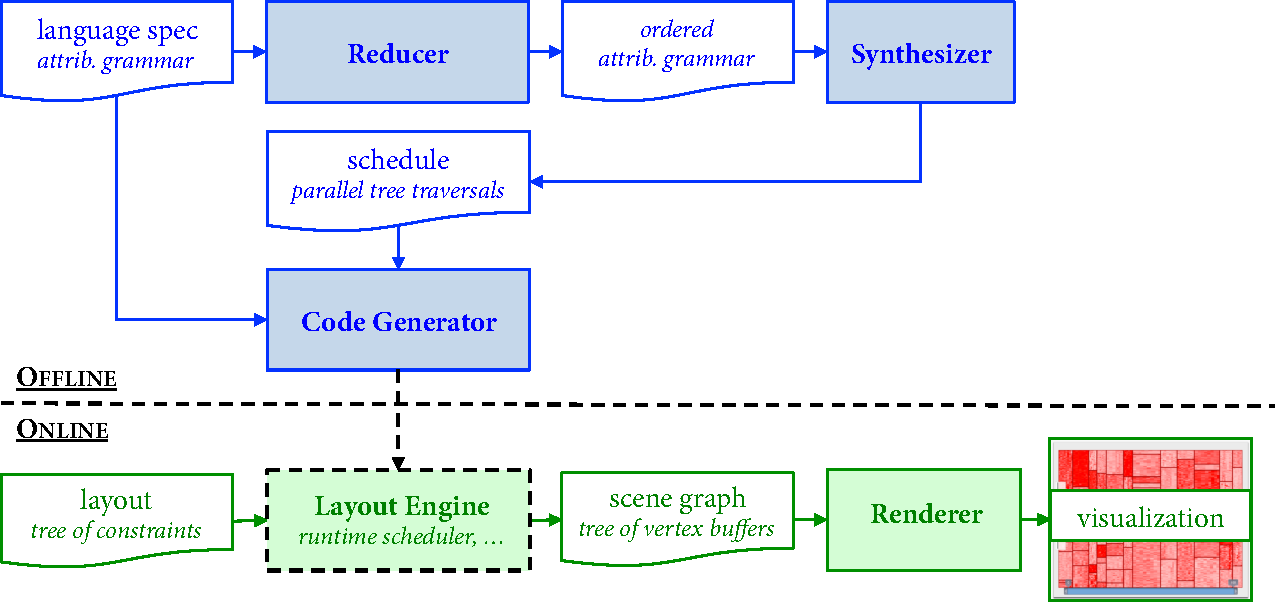
\includegraphics[trim=0 0 0 0,clip,width=1.0\columnwidth]{chapter2/architecture}
\caption{\textbf{Layout engine architecture.} }
\label{fig:architecture}
\end{figure}

Our idea is to declaratively specify layout languages and automatically compile them into an efficient implementation. At runtime, an instance of layout will be processed through the previously generated layout engine (Figure~\ref{fig:architecture}). The compiler is responsible for checking the semantics of the layout features and, by construction, provides a correct implementation. Furthermore, instead of manually optimizing the code for every individual feature, language designers instead write generic compiler optimizations. As a similar implementation benefit, we automatically target multiple platforms for the same layout language, such as scripting languages in order to use their debuggers, and multicore and GPU languages to gain magnitudes of speedups.

We show that the attribute grammar formalism supports specification of layout languages. It is unclear how to encode complicated layout language features with the traditional formalism, so we support a rich form of attribute grammars and reduce reasoning about them to handling a more traditional formalism (reducer in Figure~\ref{fig:architecture}). The remainder of this chapter introduces the high-level attribute grammar formalism, how to specify layout languages using it, and an intuition for the reduction into a lower-level formalism.


\newsavebox{\agdef}
\begin{lrbox}{\agdef}% Store first listing
\begin{minipage}{1\columnwidth}
\setlength{\grammarparsep}{0.15cm}   % vertical distance between production rules
\setlength{\grammarindent}{1cm}
\renewcommand{\litleft}{\bfseries}
\renewcommand{\ulitleft}{\bfseries}
\renewcommand{\superscript}[1]{\ensuremath{^{\textrm{#1}}}}
\renewcommand{\subscript}[1]{\ensuremath{_{\textrm{\uppercase{#1}}}}}
\renewcommand{\syntleft}{\normalfont\itshape}
\renewcommand{\syntright}{}
%\newcommand{\deriv}{~::=~}
\renewcommand{\deriv}{~ $\rightarrow$ ~}
\begin{grammar}
<AG> \deriv{} (<Prod> "\{" <Stmnt>? "\}")*

<Prod> \deriv{} <V> $\rightarrow$ <V>*

<Stmnt> \deriv{} <Attrib> "=" <id>(<Attrib>*) ~  | ~ <Attrib> "=" <n> ~ | ~ <Stmnt> ; <Stmnt> 

<Attrib> \deriv{} <id>.<id>
\end{grammar}
\end{minipage}
\end{lrbox}



\newsavebox{\hboxtreetext}
\begin{lrbox}{\hboxtreetext}% Store first listing
\begin{lstlisting}[language=C++,morekeywords={spawn,join,reverse,parallel_for}]
<S>
  <HBox name=child>
    <HBox name=left>
      <HBox name=left w=20 h=5/>
      <HBox name=right w=15 h=5/>
    </HBox>
    <HBox name=right w=15 h=5/>
  </HBox>
</S>
\end{lstlisting}
\end{lrbox}


\begin{figure}
\subfloat[\textbf{Input tree.} Only some of the x, y, w, and h attributes are specified.]{\label{fig:hbox:input}
\begin{minipage}{1\columnwidth}\centering
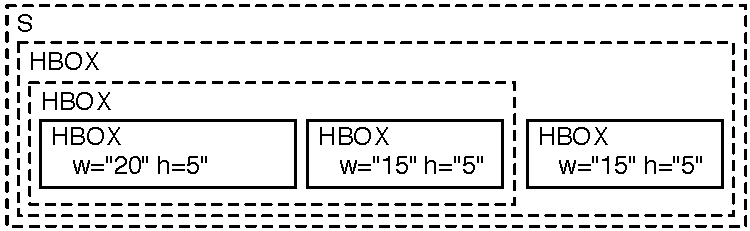
\includegraphics[trim=0 0 0 0,clip,width=0.6\columnwidth]{chapter2/output}
\end{minipage}}\\
\subfloat[\textbf{Textual encoding of input tree.}]{\label{fig:hbox:texttree}
\begin{minipage}{1\columnwidth}\centering
\usebox{\hboxtreetext}
\end{minipage}
}\\
\subfloat[\textbf{Attribute grammar for a language of horizontal boxes.}]{\label{fig:hbox:grammar}
\begin{minipage}{1\columnwidth}
\begin{grammar}
<S> \deriv{} \emph{HBOX} \\ 
  \{ HBOX.x = 0; HBOX.y = 0 \}

<HBOX> $\rightarrow$ $\epsilon$  \\
\{ HBOX.w = input$_w$(); HBOX.h = input$_h$() \} 

<HBOX$_0$> $\rightarrow$ \emph{HBOX$_1$} \emph{HBOX$_2$} \\
\{ HBOX$_1$.x = HBOX$_0$.x; \\
$~~~$ HBOX$_2$.x = HBOX$_0$.x + HBOX$_1$.w; \\
$~~~$ HBOX$_1$.y = HBOX$_0$.y; \\
$~~~$ HBOX$_2$.y = HBOX$_0$.y; \\
$~~~$ HBOX$_0$.h = max(HBOX$_1$.h, HBOX$_2$.h); \\
$~~~$ HBOX$_0$.w = HBOX$_1$.w + HBOX$_2$.w \} 
\end{grammar}
\end{minipage}
}\\
\subfloat[\textbf{Language of attribute grammars.}]{\label{fig:ag}
\usebox{\agdef}
}
\caption{For a language of horizontal boxes: (a) input tree to solve and (b) attribute grammar specifying the layout language. Specification language of attribute grammars shown in (c).%and (c) dynamic data dependencies.
}
\label{fig:hbox}
\end{figure}


\section{Background: Layout with Classical Attribute Grammar}

This section describes specifying a simple layout language as an attribute grammar and two classical implementation strategies. We reuse the example throughout our work to explore various concepts.



\subsection{Attribute Grammars}

Consider solving the tree of horizontal boxes shown in Figure~\frefb{fig:hbox}{fig:hbox:input}. As input, a webpage author provides a tree with constraints (Figure~\frefb{fig:hbox}{fig:hbox:text tree}). Only some node attribute values are provided: in this case, only the widths and heights of leaf nodes. The meaning of a horizontal layout is that, as is visualized, the boxes will be placed side-by-side. The layout engine must solve for all remaining x, y, width, and height attributes. 

We declaratively specify the layout language of horizontal boxes, \hlang{},  as shown in Figure~\frefb{fig:hbox}{fig:hbox:grammar}, with an attribute grammar~\cite{oag,Meyerovich:2010,htmlag}. First, the specification defines the set of well-formed input trees as the derivations of a context-free grammar. We use the standard notation~[[CITE]]. In this case, a document is an unbalanced binary tree of arbitrary depth where the root node has label \texttt{S} and intermediate nodes have label \texttt{HBOX}. Second, the specification defines semantic functions that relate attributes associated with each node. For example, the width of an intermediate horizontal node is the sum of its children widths. Likewise, the width of a leaf node is provided by the user, which is encoded by the nullary function call $input_w()$:


\begin{grammar}
<HBOX> $\rightarrow$ $\epsilon$ \{ HBOX.w = $input_w$(); $\ldots$ \} ~~~~~~~~~~~~~~~~~~~~~~~ /* leaf */

<HBOX$_0$> $\rightarrow$ \emph{HBOX$_1$} \emph{HBOX$_2$} ~~~~~~~~~~~~~~~~~~~~~~~~~~~~~~~~~ /* binary node */\\
\{ $\ldots$ HBOX$_0$.w = HBOX$_1$.w + HBOX$_2$.w \} 
\end{grammar}


The specification intentionally does not define the evaluation order. For example, the specification does not state whether to compute a node's width before its height. Likewise, our optimized approach will compute the attributes as a sequence of tree traversals, but the specification does not state what those traversals are. Leaving the evaluation order unspecified provides freedom for our compilers to pick an efficient parallel order. Irrespective of whatever evaluation order is ultimately used to solve for the attribute values, the statements define constraints that must hold over the computed result. Attribute grammars can therefore be thought of as a single assignment language where attributes are dataflow variables~[[CITE]].


The language of attribute grammars is defined in Figure~\frefb{fig:hbox}{fig:ag}. In addition the defining the context free grammar, it supports single-assignment constraints over attributes of nodes in a production. Our example uses the following encoding. Semantic functions are pure and left uninterpreted, so, for example, we encode the addition of widths as ``\mbox{HBOX$_0$.w = f(HBOX$_1$.w, HBOX$_2$.w)}''. Our program analysis techniques do not need to know the contents of the function, just that the output of a call depends purely on the inputs.  For the same reason, we encode constant values as nullary function calls. 

To specify grammars more complicated than \hlang{}, we describe linguistic extensions for richer functional specifications (Section~\ref{sec:desugaring}) and, to control the evaluation order, behavioral specification (Chapters~\ref{chap:3} and \ref{chap:4}).

\begin{figure}
\subfloat[Initial dependencies.]{\label{fig:deps:full}
\begin{minipage}{0.5\columnwidth}\centering
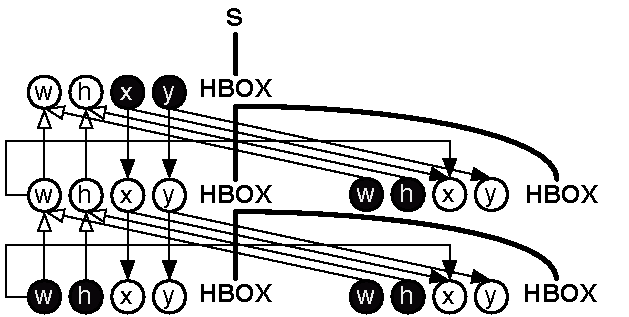
\includegraphics[trim=0 0 0 0,clip,width=1.0\columnwidth]{chapter2/deps}
\end{minipage}}
\subfloat[After first round of evaluation.]{\label{fig:deps:step}
\begin{minipage}{0.5\columnwidth}\centering
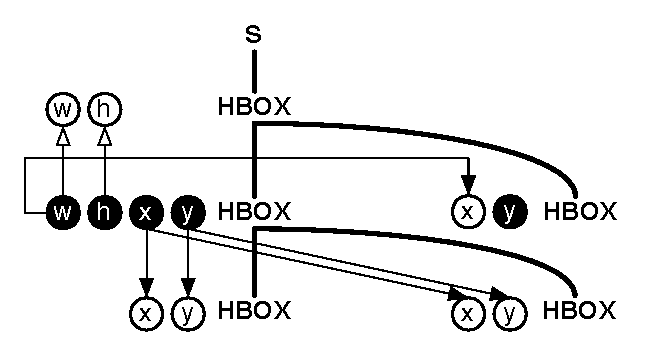
\includegraphics[trim=0 0 0 0,clip,width=1.0\columnwidth]{chapter2/depsstep}
\end{minipage}}
\caption{\textbf{Dynamic data dependencies and evaluation}. Shown for constraint tree  in Figure~ZZZ~(a). Circles denote attributes, with black circles denote attributes with resolved dependencies such as \sched{input()}s. Thin lines show data dependencies and thick lines show production derivations. Second chart shows the dependency graph resulting from evaluating all source nodes and marking them as resolved.}
\label{fig:deps}
\end{figure}


\subsection{Dynamic data dependencies and dynamic evaluation}
A simple and classic evaluation strategy is to \emph{dynamically} compute over a tree. The evaluator dynamically follows the dynamic data dependencies between instances of attributes. The dynamic evaluation strategy is too slow for our use cases, but it introduces the key concepts of dynamic data dependencies, the dynamic semantics of attributes grammars, and the corresponding dynamic interpreter.

An instance of a document corresponds to the dependency graph shown in Figure~\frefb{fig:reps}{fig:deps:full}. Each attribute of a tree node is either a source, meaning its value can be computed based on other known values, or it cannot be evaluated until other attribute values are known. It is a dynamic dependency graph in that each data dependency in the static code may be instantiated as multiple data dependencies given a tree at runtime. 

The dynamic data dependency graph leads to a simple semantics for the result of evaluation. The graph corresponds to a system of equations where edges link instance variables. For example, static code \code{HBOX$_2$.x = HBOX$_0$.x + HBOX$_1$.w} instantiates twice for the Figure~\frefb{fig:deps}{fig:reps:full}: once for each $x$ attribute with an incoming elbow connector. The value of both $x$s are constrained by distinct instances of the above constraint. If the dependency graph is a directed acyclic graph and each attribute appears on the lefthand side of exactly one equality statement (\emph{dataflow variables}), there is exactly one solution to the system of equations.

A simple procedure solves an instance of a system of equations: topological traversal. The algorithm is as follows:
\begin{figure}
\begin{lstlisting}[mathescape,language=C++,morekeywords={for,in,where,input,output,repeat,until,return}]
input: $G = (V,E)$
output: $Map$
$Map \leftarrow \emptyset$
$E' \leftarrow E$
$V' \leftarrow V$
for $a \in V' \texttt{where} \not\exists (n,a) \in E'$:
  $Map \leftarrow Map \cup \{a \rightarrow \texttt{eval}(a)\}$
  $V' \leftarrow V' - a$
  $E' \leftarrow E' \ (\{a\} \times V)$
repeat until $E' = \emptyset$
return $Map$
\end{lstlisting}
\caption{\textbf{Dynamic attribute grammar evaluator.} It selects attributes in a safe order by dynamically removing dependency edges as they are resolved. }
\label{fig:dyneval}
\end{figure}
The algorithm literately finds an attribute whose dependencies have all been previously resolved, evaluates the attribute, and repeats. If the input graph is a directed acyclic graph, this procedure is guaranteed to terminate. The insight is that a directed acyclic graph has at least one fringe node, the loop removes them, and removing these nodes yields a smaller directed acylic graph.

The dynamic evaluation strategy provides a small explanation for the natural semantics, but it leaves several challenges. First, runtime manipulation of a dynamic dependency graph introduces high overheads because every dynamic dependency edge must be manipulated. Second, it is unsafe. For example, a cycle in the dependency graph causes the above evaluation strategy to get stuck, so dynamic evaluators must introduce runtime cycle check. Designers can build layout widgets that, depending on how they are invoked, fail to display!

%\subsection{Static data dependencies and static evaluators}




\section{Desugaring Loops and Other Modern Constructs}
\label{sec:desugaring}

The attribute grammar formalism was invented for describing semantics~[[CITE]] and before many modern constructs became mainstream: we had to design extensions for improved expressiveness and maintainability. Our extensions exploit concepts from structured, object-oriented, and functional programming. Other language designers have build such extensions as well~[[CITE]]: our challenge was to make expressive extensions that facilitate effective parallelization and do not overly complicate language and tool implementation. This section documents the language features and how they simplify implementation, and leaves performance optimization to the next chapter.

Our key insight is that pre- and post-processing supports desugaring a feature-rich attribute grammar into the canonical attribute grammar notation. Tools then operate at the most appropriate stage, such as our scheduler on the small, canonical attribute grammar representation. Likewise, our code generators take a generated schedule and relate it back to a representation from early in the preprocessing stage. Many of the below features are built as explicit compiler stages, but over time, we found that declarative tree rewriting systems such as ANTLR and OMeta support automating individual stages.



\newsavebox{\ifacegrammar}
\begin{lrbox}{\ifacegrammar}% Store first listing
\begin{lstlisting}[language=C++,morekeywords={interface,class,children}]
interface BoxI { }
class HBoxLeaf : BoxI { }
class HBoxBinary : BoxI { 
  children {
    left: BoxI;
    right: BoxI;
  }
}
class VBoxLeaf : BoxI { }
class VBoxBinary : BoxI { 
  children {
    left: Box;
    right: Box;
  }
}
\end{lstlisting}
\end{lrbox}




\begin{figure}
\subfloat[\textbf{Canonical attribute grammar.}]{\label{fig:iface:problem}
\begin{minipage}{1\columnwidth}
\begin{grammar}
<S> \deriv{} \emph{HBOX}  $|$  \emph{VBOX}

<HBOX> \deriv{} $\epsilon$  

<HBOX$_0$> \deriv{} \emph{HBOX$_1$} \emph{HBOX$_2$} 

<HBOX$_0$> \deriv{} \emph{VBOX$_1$} \emph{HBOX$_2$} 

<HBOX$_0$> \deriv{} \emph{HBOX$_1$} \emph{VBOX$_2$} 

<HBOX$_0$> \deriv{} \emph{VBOX$_1$} \emph{VBOX$_2$} 

<VBOX> \deriv{} $\epsilon$  

<VBOX$_0$> \deriv{} \emph{HBOX$_1$} \emph{HBOX$_2$} 

<VBOX$_0$> \deriv{} \emph{VBOX$_1$} \emph{HBOX$_2$} 

<VBOX$_0$> \deriv{} \emph{HBOX$_1$} \emph{VBOX$_2$} 

<VBOX$_0$> \deriv{} \emph{VBOX$_1$} \emph{VBOX$_2$} 

\end{grammar}
\end{minipage}
}\\
\subfloat[\textbf{Interface sugar.}]{\label{fig:iface:clean}
\usebox{\ifacegrammar}
}\\
\subfloat[\textbf{Interface encoding.}]{\label{fig:iface:rewrite}
\begin{minipage}{1\columnwidth}
\begin{grammar}
<S> \deriv{} \emph{BOX}

<BOX> \deriv{} \emph{HBOX} $|$ \emph{VBOX}

<HBOX> \deriv{} $\epsilon$  

<HBOX$_0$> \deriv{} \emph{BOX$_1$} \emph{BOX$_2$} 

<VBOX> \deriv{} $\epsilon$  

<VBOX$_0$> \deriv{} \emph{BOX$_1$} \emph{BOX$_2$} 

\end{grammar}
\end{minipage}
}
\caption{\textbf{Interfaces for tree grammars}. Subfigures show manually encoding multiple production right-hand sides, an encoding that uses a \code{Box} non-terminal for indirection, and the high-level encoding using interfaces and classes.}
\label{fig:iface}
\end{figure}


\begin{figure}
\begin{lstlisting}[language=C++,morekeywords={spawn,join,reverse,parallel_for}]
{"class": "HBox",
 "children": {
   "left": {
     "class": "HBox",
     "children": {
       "left":  {"class": "HBox", "w": 20, "h": 5},
       "right": {"class": "HBox", "w": 15, "h": 5}}},
   "right": {
     {"class": "HBox", "w": 15, "h": 5}}}}
\end{lstlisting}
\caption{\textbf{Input tree as graph with labeled nodes and edges}. Specified in the JSON notation.}
\label{fig:hboxjson}
\end{figure}

\subsection{Interfaces for Encoding Tree Grammars}
Attribute grammars are an extension to the tree grammar formalism for defining input trees, so improving the abstraction capabilities of tree grammars also aids the ability to structure attribute grammars. In particular, we found the need to support  abstracting over similar types of non-terminals. Our solution is to provide a notion of classes and interfaces. Our core extension is macro-expressible with attribute grammars and therefore reduces implementation requirements, though it is still important enough that it merits deeper compiler support. 


Consider the code duplication performed when extending \hlang with vertical boxes. The children of a \code{HBox} could be a horizontal box or a vertical box, and the same for the children of a vertical box. Figure~\ref{fig:face:problem} shows that the 3 productions of \hlang grew to be 11. The example highlights that canonical attribute grammars cannot abstract over node types. Adding a new box type requires modifying all previous box classes, and in the presence multiple children, extension suffers exponential costs. 

To abstract over node types, we introduce the notion of classes and interfaces (Figure~\ref{fig:iface:clean}). Classes are similar to the productions of an attribute grammar: the class name specifies the production's lefthand side non-terminal and the children block specifies the production's righthand side. Unlike attribute grammars, an interface name is used for the righthand side rather than the class name. \code{HBox} and \code{VBox} implement interface \code{BoxI}, so any class specified to have a \code{BoxI} child can have a \code{HBox} or \code{VBox} child within the concrete tree. 


Classes and interfaces are formally equivalent to tree grammars in the sense of a 1-to-1 correspondence between trees described by both. First, a tree grammar can be expressed with classes and interfaces by treating all productions with the same lefthand-side non-terminal as different classes belonging to the same interface. In the other direction, each interface can be expressed as a production that derives the classes, and the classes expand into productions. Figures~\ref{fig:iface:clean} and \ref{fig:iface:rewrite} demonstrate the correspondence for \hlang. The induced implementation requirements are therefore slight in the sense that the construct is sugar for a pattern in the canonical attribute grammars. 

We depart from the correspondence for the encoding of trees in two ways. First, we represent input as a tree with labeled nodes and edges. Node labels denote the class and edge labels specify child bindings. Figure~\ref{fig:hboxjson} uses the JSON format common to dynamic languages for an instance of a tree in \hlang. By naming children, such as \code{left} and \code{right}, we eliminate sensitivity to their order within a code block. With order sensitivity, adding a middle child \code{center} would needlessly require refactoring references to the repositioned element \code{right}. Likewise, reordering children in the input data does not require refactoring the attribute grammar.

Our second departure from the canonical attribute grammar encoding optimizes the data representation by eliding intermediate interface nodes. The reduction to attribute grammars suggests adding a new non-terminal for each interface, but doing so in the data representation doubles the number of nodes in the concrete tree. Making the interface pattern a language construct with compiler support eliminates associated costs, such as cutting file size for runtime parsing of big data visualizations.

\begin{figure}
\begin{lstlisting}[language=C++,morekeywords={interface,class,var,input,int,float}]
interface BoxI {
  var x : float;
}
class HBoxLeaf : BoxI {
  attributes {
    var y : int;
    input w : ? int;
    input h : int = 10;
  }
}


\end{lstlisting}
\caption{\textbf{Input tree as graph with labeled nodes and edges}. Specified in the JSON notation.}
\label{fig:hboxjson}
\end{figure}


\subsection{Interfaces for attributes and information hiding.}
Our system provides lightweight specification annotations for different types of attributes, and coupled with the interface construct, it supports defining relationships between attributes across different classes.

Each static attribute is annotated with its assignment type and its embedded value type:
\begin{itemize}
\item \textbf{Assignment types.}
The assignment type denotes whether the input tree defines the value, such as in \code{input w}, or whether the attribute grammar defines it, as in \code{var x}. Assignments to an input type are illegal, and multiple assignments to a variable type are also illegal. 

If an input tree fails to provide an input attribute, a runtime error will be thrown. To still provide an interpretation of such trees, input attributes  support the annotation ''?'',  which enables pattern matching through functions \code{maybeReady :: -> boolean} and \code{maybeValue :: -> 'a}.  Alternatively, for the common scenario of using a fixed default value, a default value can instead be defined as in \code{input h : int = 10}. If the input tree does not provide the value, the default value will be automatically substituted.

Canonical attribute grammars can encode input attributes in two ways. First, semantic functions with no parameters encode the lack of dependencies. Second, for finite domains, the set of tree grammar productions can expand to include attribute nodes. The second encoding more faithfully describes our approach because, like our system, it feeds into an automatic tree parser generator. For each tree node, our generated parser scans for the expected set of input attributes.

\item \textbf{Value types.} 
The system also supports type annotations used for embeddings. Generated code typically compiles as part of a project in a more static language, such as C++, which require a static type discipline. The annotations can be user-defined, such as OpenGL's \emph{vertex buffer object} \code{VBO}, which is not defined within our system.

Our analyzer ignores the value type annotations such as \code{x : float} and \code{y : int} while the low-level code generator passes along the decorations \code{float} and \code{int}.  The embedded design simplifies implementation because value type checking is performed by the host language's compiler. 
\end{itemize}

In practice, we  use attribute definitions in interfaces for information hiding across classes and lightweight specification of relationships between similar classes. An attribute declared inside of a class is \emph{local} to constraints in the class: only the class's constraints can read or write to the attribute. Conversely, declaring a \emph{var} inside of an interface hints that it is meant to be reused by outside classes, such as part of a tree traversal.

\begin{figure}
\begin{lstlisting}[language=C++,morekeywords={trait,class,attributes,actions}]
trait Rectangle {
  attributes { render : int; }
  actions { render := paintRect(x,y,w,h, "black"); }
}
class HBox(Rectangle) : BoxI { ... }
\end{lstlisting}
\caption{\textbf{Trait construct}. Adds shared rendering code to the HBox class.}
\label{fig:trait}
\end{figure}

\subsection{Traits: Reusing Cross-cutting Code}
As with many object systems, we support a trait construct for cross-cutting code that should be shared across classes. It statically expands like a macro, and therefore provides no formal expressive power. For example, Figure~\ref{fig:trait} defines how to render a rectangle given several attributes, and then adds that functionality to class \code{HBox}. If the language was extended with class \code{VBox}, the class definition of \code{VBox} could also use trait \code{Rectangle}.






\begin{figure}
\begin{lstlisting}[language=C++,morekeywords={spawn,join,reverse,parallel_for}]
interface BoxI {
  var w : int;
  var h : int;
  var right : int;
  var bottom : int;
}
class HBox : BoxI {
  children {
    childs : [ BoxI ]
  }
  actions {
      loop childs {
        w := fold 0 .. self$-.w + childs$i.w;
        h := fold 0 .. max(self$-.h, childs$i.h)
        childs.right := fold x .. childs$-.right + childs$i.w;
        childs.bottom := fold y .. childs$-.bottom + childs$i.h;  
      }
  }
}
\end{lstlisting}
\caption{\textbf{Input tree as graph with labeled nodes and edges}. Specified in the JSON notation.}
\label{fig:loops}
\end{figure}

\subsection{Loops}
We extend our language with declarative loops over the attributes of multiple nodes. They are an expressive extension over the uniform recurrence relations of [[CITE]].

The loop construct, \code{loop}, specifies a block of loop body statements. It acts over a sequence of nodes declared with the same interface, such as \code{childs : [ BoxI ]} in Figure~\ref{fig:loops}. The looping order is restricted to forward iteration, though our approach generalizes to other loop orders.

A statement in a loop body will execute for each element of the list. For example, the following statement assigns the attribute \code{w} the sum of the children widths:
\code{w := fold 0 .. self\$-.w + childs\$i.w}
Similar to array index notation, the suffix on righthand-side variable names for loop statements provide a restricted form of relative indexing for loops. In particular:
\begin{itemize}
\item \$i: the ``current'' loop step
\item \$-: the previous loop step
\item \$\$: the last loop step
\end{itemize}
Use of suffix ``\$-'' in a \code{fold} can be thought of as an accumulator in functional programming. 


One loop statement can refer to the accumulator of another, which fold statements in most languages do not support. For example, two loop counters can be intertwined:
\begin{lstlisting}
loop childs {
  childs.counter1 := fold 0 .. childs$-.counter2 + 1;
}
loop childs {
  childs.counter2 := fold 0 .. childs$-.counter1 + 1;
}
\end{lstlisting}
The programmer does not need to order the statements.  For example, our system infers that the imperative code that implements the above declarations is just one imperative loop that fuses them together. The incorrect alternative of implementing the declarations as a different imperative loop for each would lead to unfulfilled data dependencies. The freedom in statement order supports automatic parallelization, but also allowed programmers choice in how to structure the program once machine considerations were removed.

We reduced scheduling loops to scheduling canonical attribute grammars. Our insight is that, for a restricted language of relative indices, we can schedule several unrolled loop steps and generalize the schedule to the rest. Section~\ref{???} discusses this in more detail. 

\subsection{Embedded Domain Specific Language: Functional Rendering}
We designed our system for interaction with other tools and languages. A key ability is to invoke externally-defined functions, such as \code{max()}  of Figure~\ref{fig:loops} for the maximum of two numbers and \code{paintRect()} of Figure~\ref{fig:trait} to draw a rectangle to the screen. Attribute grammars are compiled to run in some host system, such as JavaScript or OpenCL, and any function in scope to the generated code may be called.

Functions can be safely embedded as long as they provide a \emph{pure} interface. In particular, the returned output should only depend on the inputs. Likewise, functions should be reentrant for use in automatic parallelization In the case of embedding in statically checked languages, the host's static checker is responsible for checking usage.



\begin{figure}
\subfloat[\textbf{Sunburst}]{\label{fig:renderings:sunburst}
\begin{minipage}{0.5\columnwidth}\centering
\includegraphics[trim=0 0 0 0,clip,width=1.0\columnwidth]{chapter2/sunburst}
\end{minipage}}
\subfloat[\textbf{Treemap}]{\label{fig:renderings:treemap}
\begin{minipage}{0.5\columnwidth}\centering
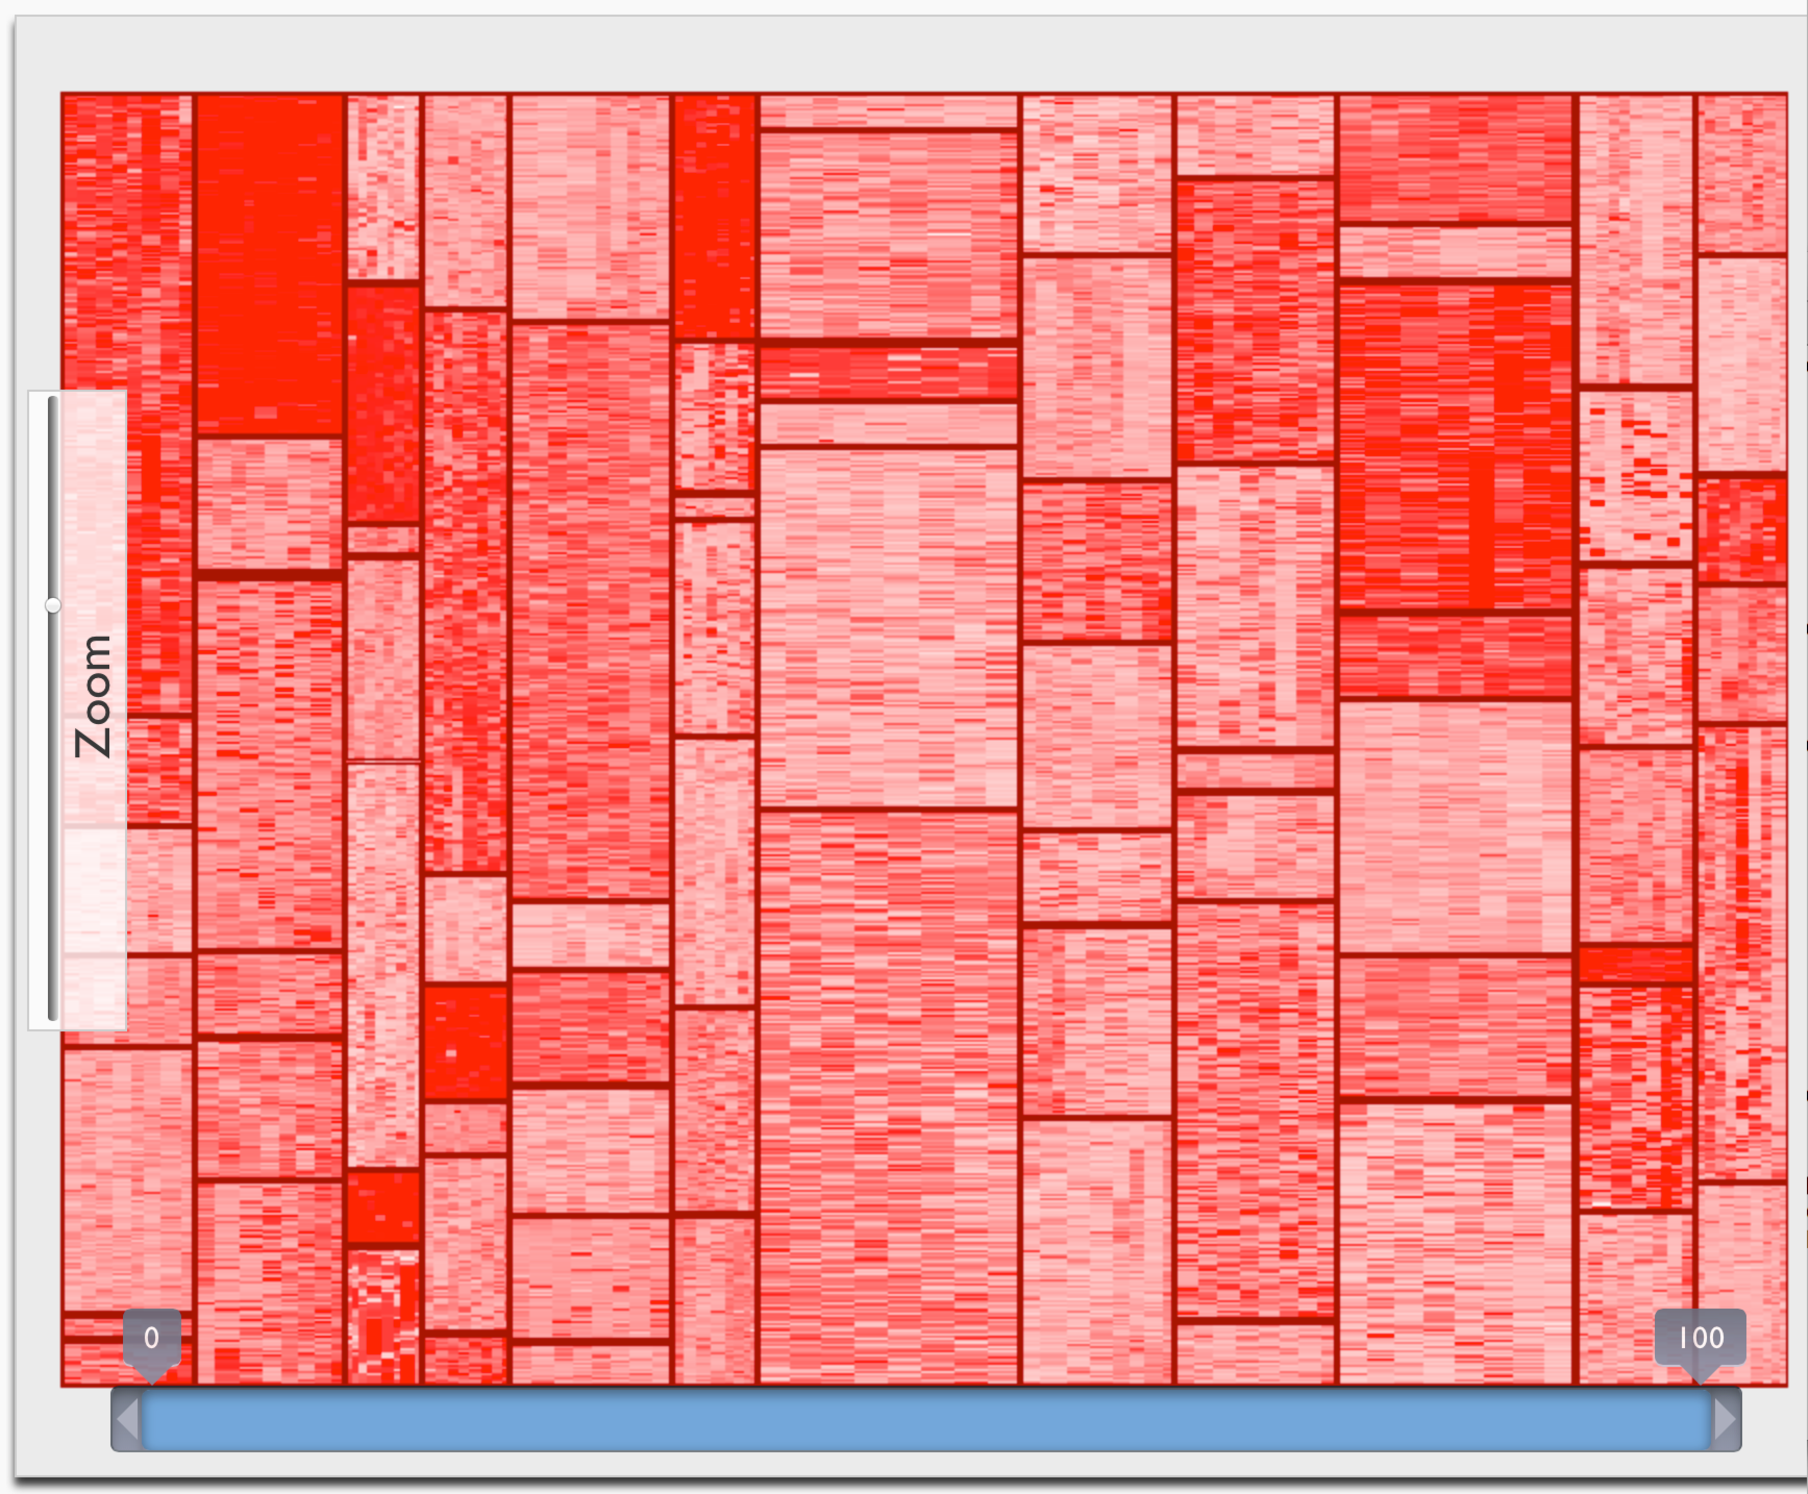
\includegraphics[trim=0 0 0 0,clip,width=1.0\columnwidth]{chapter2/election}
\end{minipage}}\\
\subfloat[\textbf{Linked Scatter}]{\label{fig:renderings:parlab}
\begin{minipage}{0.5\columnwidth}\centering
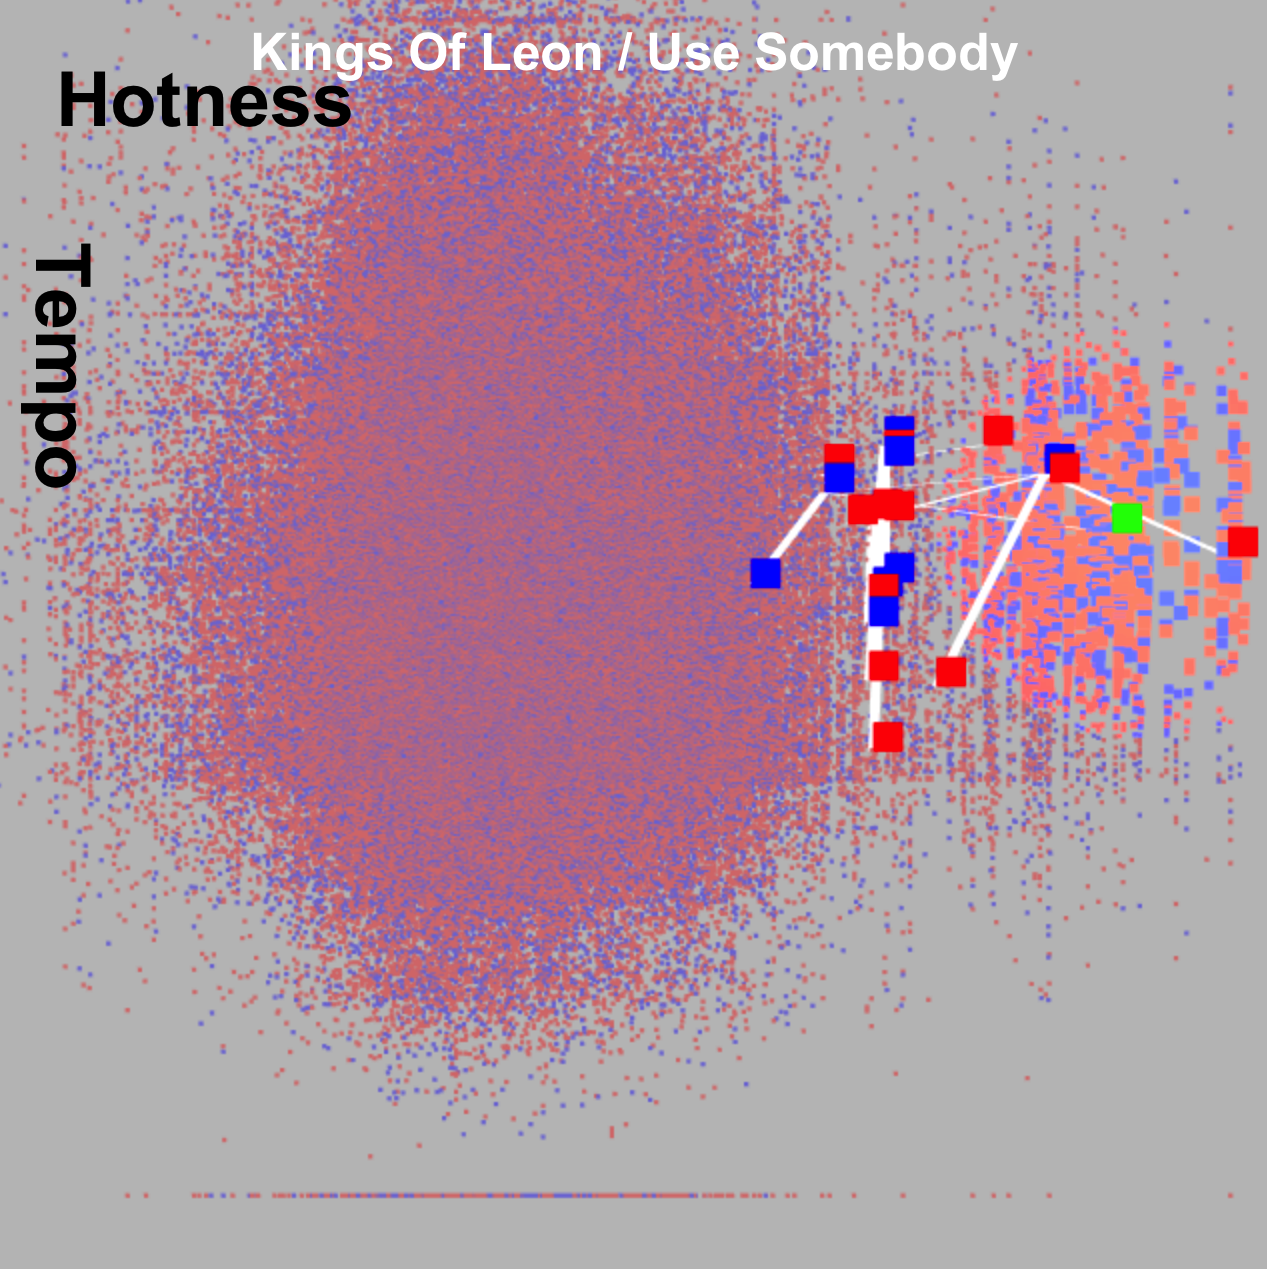
\includegraphics[trim=0 150mm 0 0,clip,width=1.0\columnwidth]{chapter2/parlabscreenshot2}
\end{minipage}}
\subfloat[\textbf{3D Multiple Time Series}]{\label{fig:renderings:ge}
\begin{minipage}{0.5\columnwidth}\centering
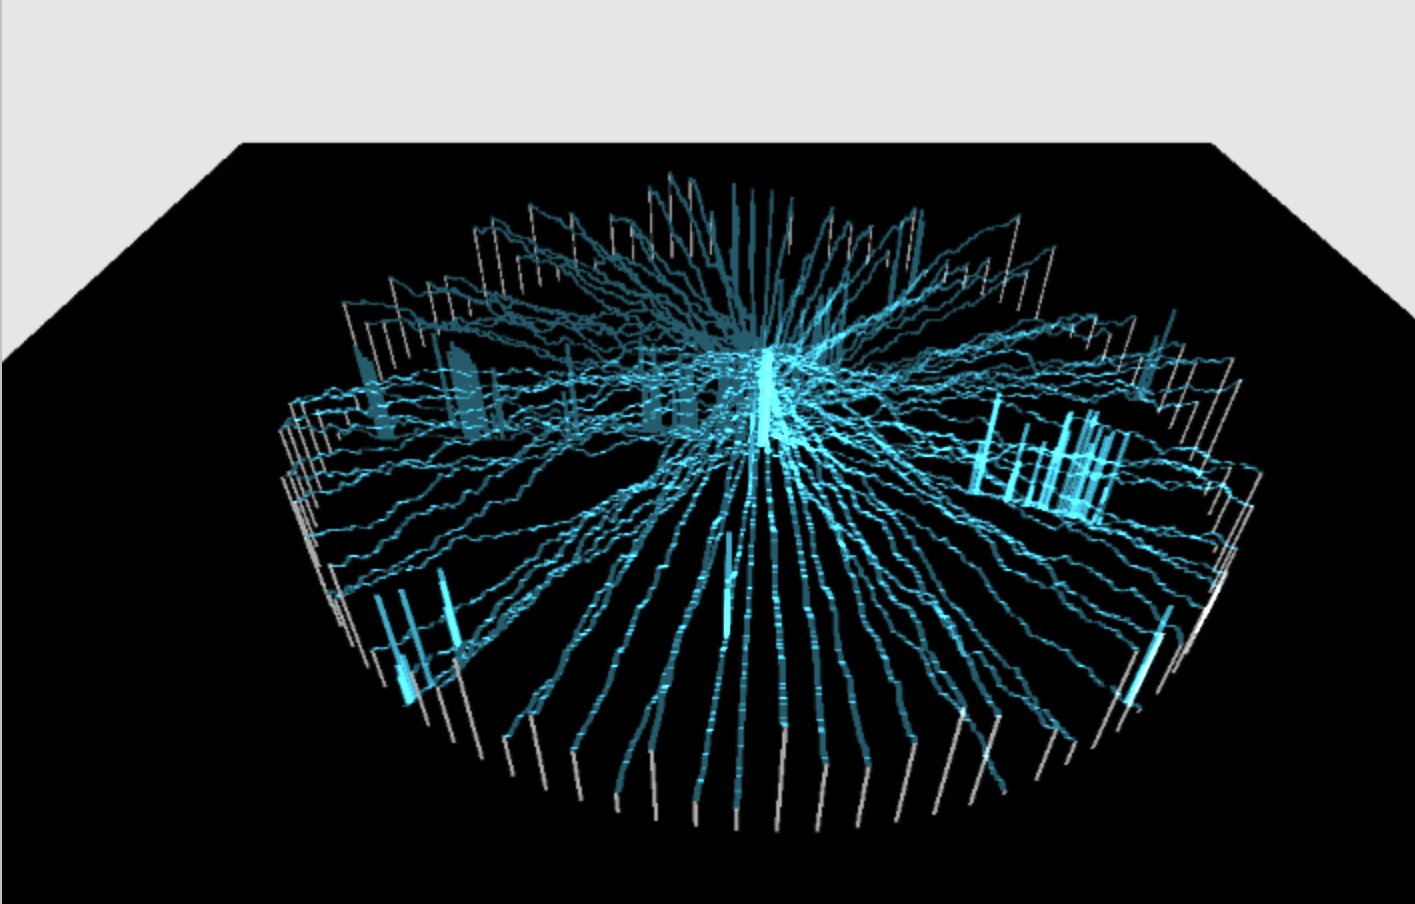
\includegraphics[trim=0 0 0 0,clip,width=1.0\columnwidth]{chapter2/ge}
\end{minipage}}\\
\subfloat[\textbf{Line Graph}]{\label{fig:renderings:line}
\begin{minipage}{1.0\columnwidth}\centering
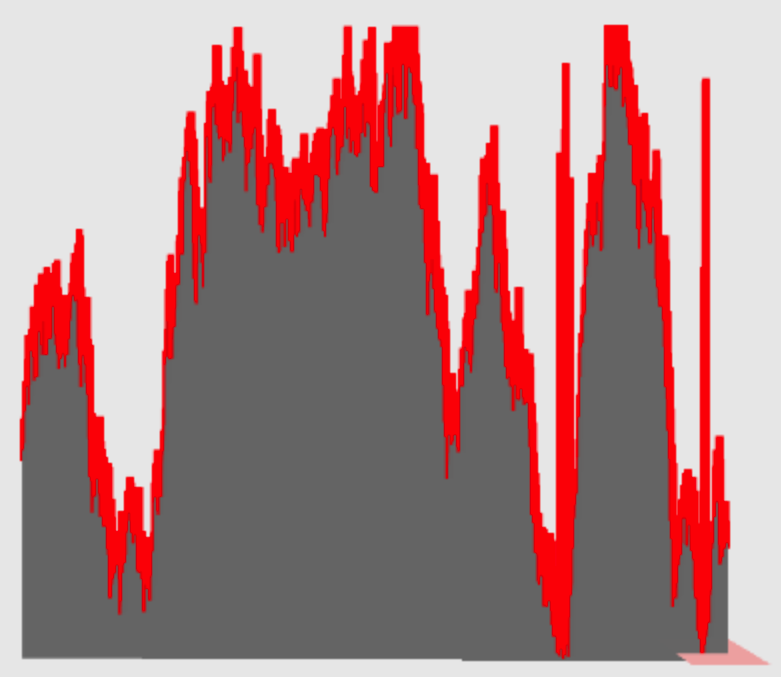
\includegraphics[trim=0 0 0 0,clip,width=0.35\columnwidth]{chapter2/line}
\end{minipage}}
\caption{\textbf{Visualization screenshots.} All except [[CITE]] are interactive or animated. Each one was declaratively specified with our extended form of attribute grammars and automatically parallelized. Labels describe whether GPU or multicore code generation was used.}
\label{fig:vizrenderings}
\end{figure}

\begin{figure}
\subfloat[\textbf{HTML Tables} (grid-based)]{\label{fig:renderings:tables}
\begin{minipage}{1.0\columnwidth}\centering
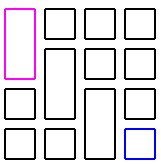
\includegraphics[trim=0 0 0 0,clip,width=0.3\columnwidth]{chapter2/table}
\end{minipage}}\\
\subfloat[\textbf{CSS} (flow-based)]{\label{fig:renderings:css}
\begin{minipage}{1.0\columnwidth}\centering
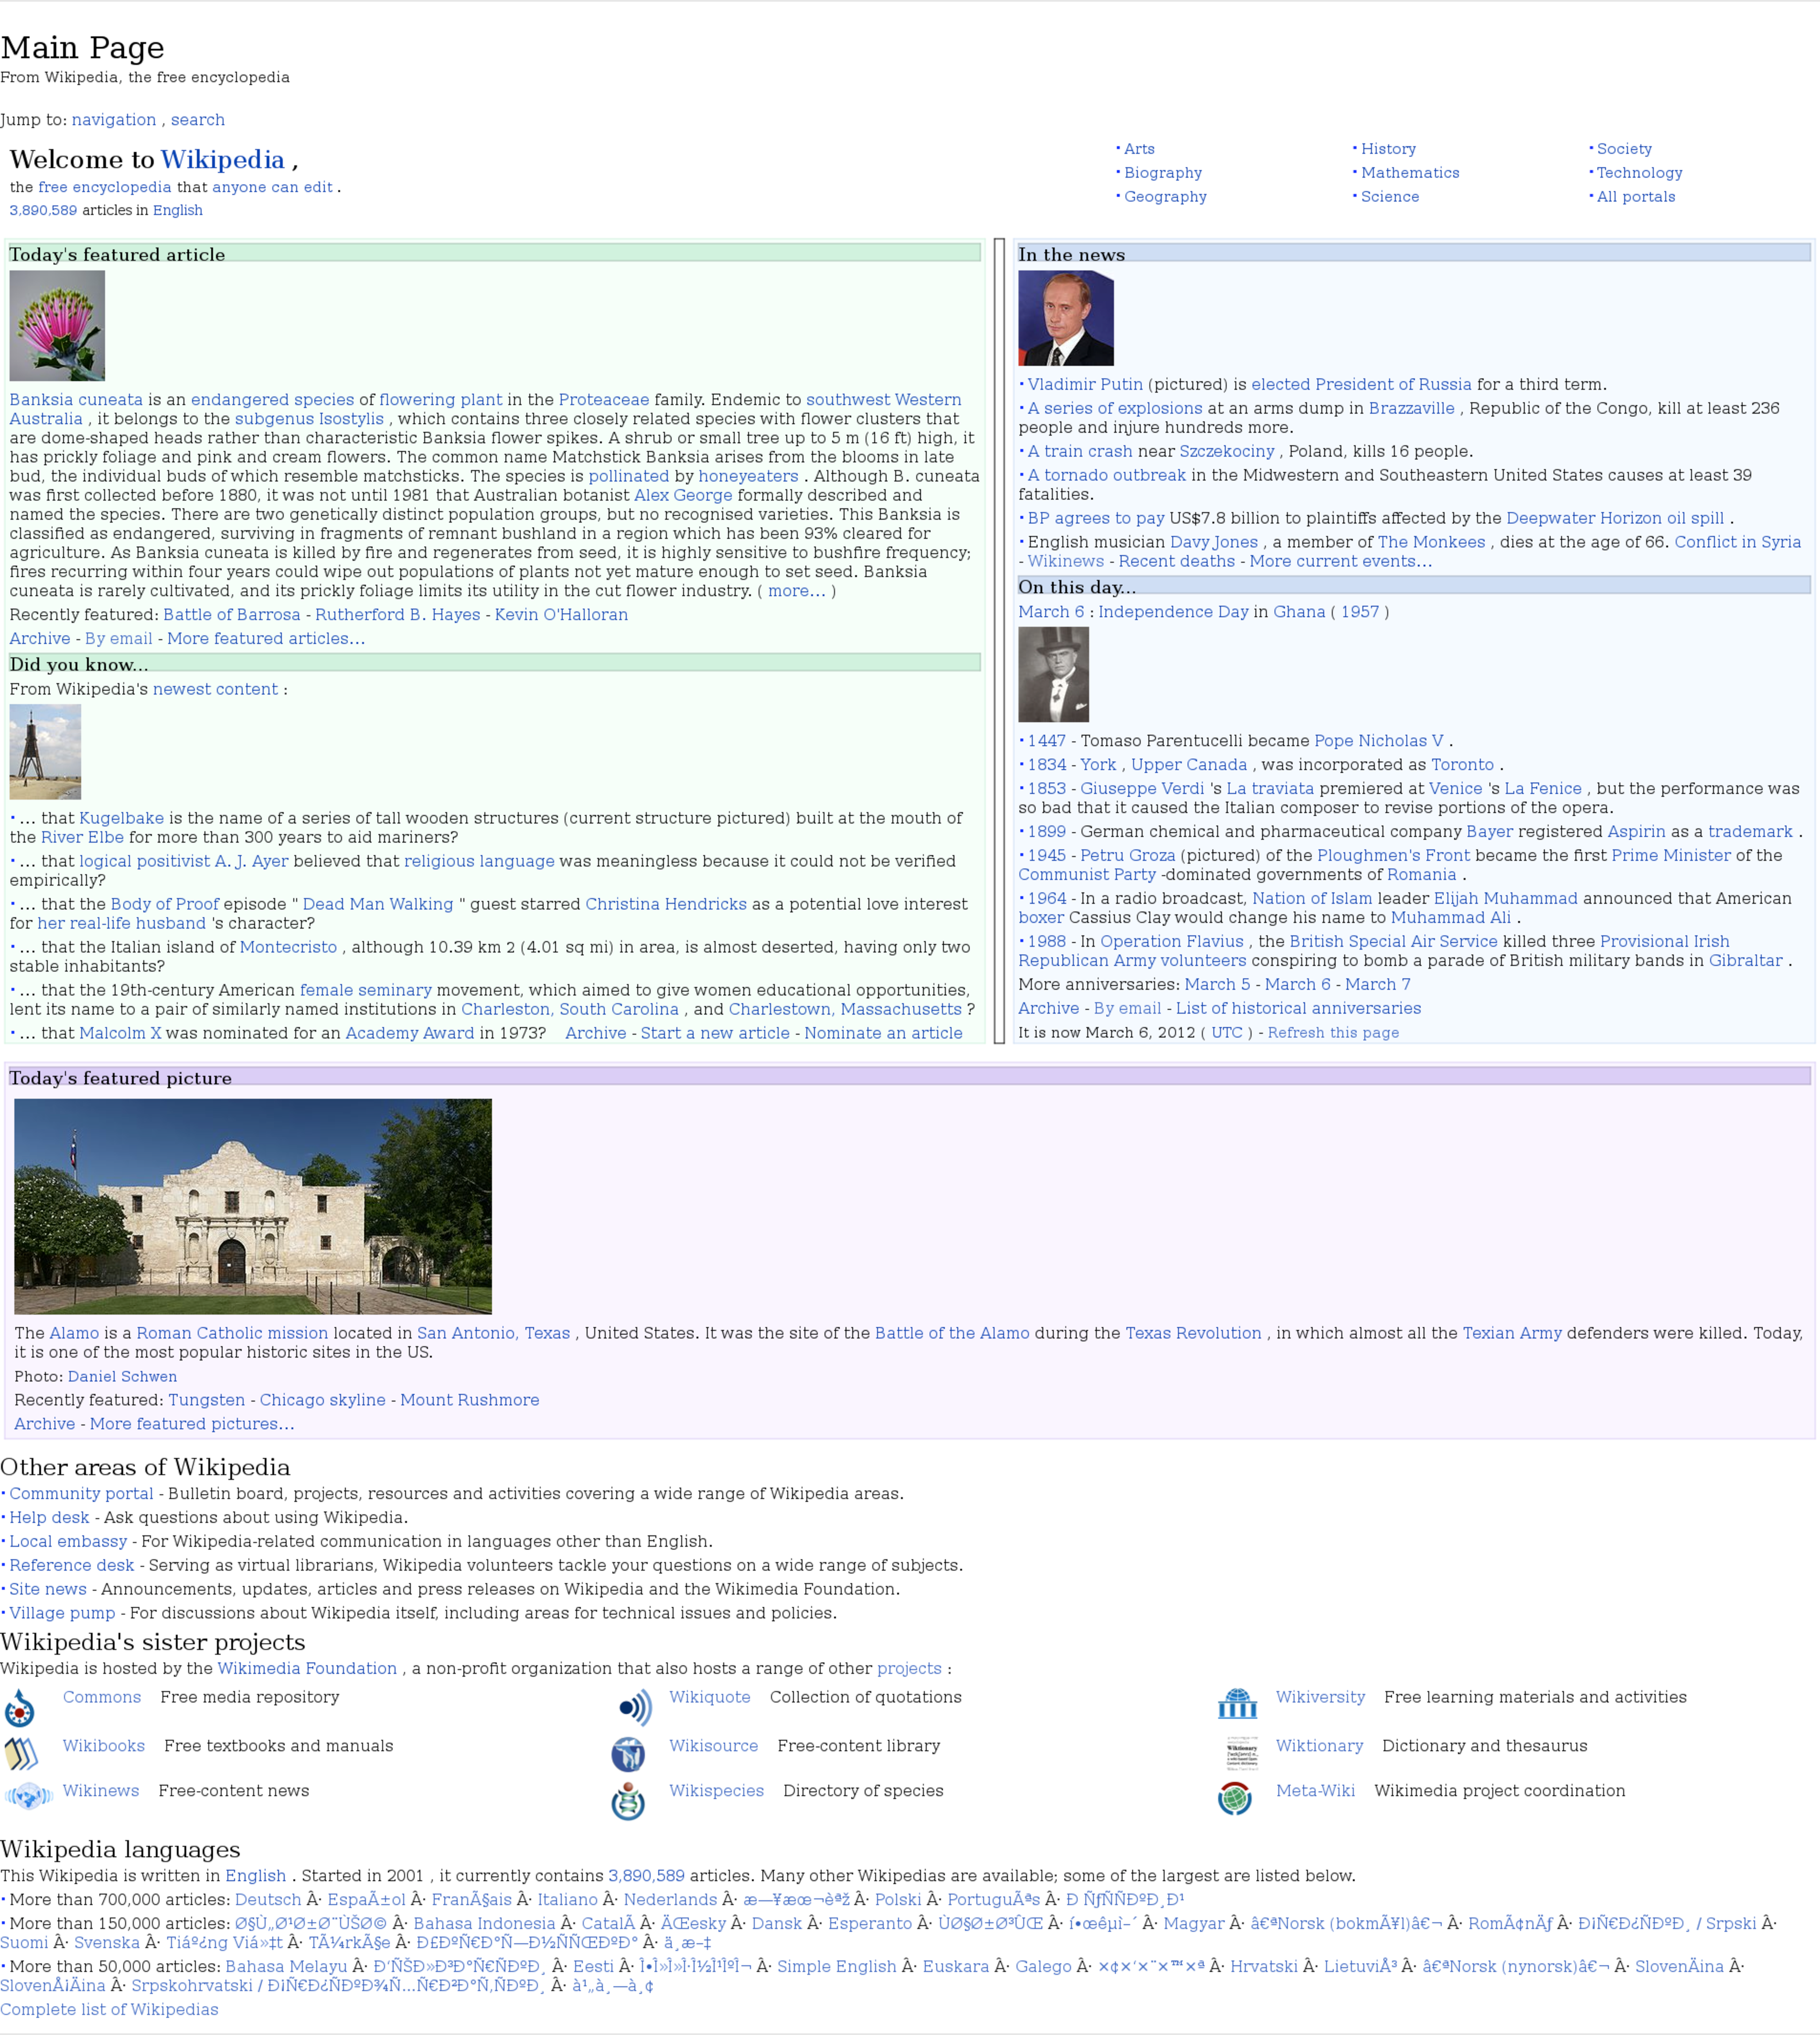
\includegraphics[trim=0 0 0 0,clip,width=0.8\columnwidth]{chapter2/wiki}
\end{minipage}}
\caption{\textbf{Document layout screenshots.}}
\label{fig:docrenderings}
\end{figure}




\section{Evaluation: Mechanized Layout Features}
We specified many common layout language features with our extended form of attribute grammars. Most examples were written with few, if any, modifications to the generated code. This experience shows that our restricted form of attribute grammars are a viable formalism for layout specification. The following subsections present highlights from our case studies in specifying layouts with attribute grammars, and the appendix contains the full code.

\subsection{Rendering}
\label{sec:rendering}
We found several rendering patterns to be important for many visualizations. A library of functional graphics primitives, such as \code{paintRect} in Figure~\ref{fig:trait}, sufficiently augmented our attribute grammar language in order to achieve them.

\begin{itemize}
\item \textbf{2D and 3D.} Our base primitives are 3D, and we provide 2D primitives that reduce into them. 
\item \textbf{Color.} Our functional graphics primitives take an RGBA value as input, which enables controlling hue, luminosity, and opacity.
\item \textbf{Linked view}. Multiple renderable objects can be associated with one node, which we can use for providing different views of the same data. Such functionality is common for statistical analysis software:

\begin{lstlisting}[mathescape]
render :=  Circle(x,y,r)  + Circle(offsetX + abs(x), offsetY + abs(y), r);
\end{lstlisting}

\item \textbf{Zooming.} We can use the same multiple representation capability for a live zoomed out view (``picture-in-picture''):

\begin{lstlisting}[mathescape]
render :=  
  Circle(x, y, radius) 
   + Circle(xFrame + x*zoom, yFrame + y*zoom, radius *zoom);
\end{lstlisting}

\item \textbf{Visibility toggles.} Our macros support conditional expressions, which enables controlling whether to render an object. For example, a boolean input attribute can control whether to show a circle: \code{render := isOn ? Circle(0,0,10) : 0; }
\item \textbf{Alternative representations.} Conditional expressions also enable choosing between multiple representations, not just on/off visibility:
\begin{lstlisting}[mathescape]
render := 
  isOff ? 0
    : mouseHover ? CircleOutline(0,0,10) 
    : Circle(0,0,10,5) ;
\end{lstlisting}

\end{itemize}


\subsection{Non-Euclidean: Sunburst Diagram}
Visualizations often require non-Euclidean layouts, such as the polar layout for the Sunburst diagram. Instead of propagating and computing over Euclidean values such as x and y coordinates as in \hlang, the visualization can use some other.

For example, in a sunburst diagram (Figure~\ref{fig:renderings:sunburst}), a node should be rendered  far from the center of the chart if its level is high. In our implementation, each node transitively computes its  radius as a function of its parent's. Likewise, the center of visualization propagates from parent to child, with the root node representing the center:

\begin{lstlisting}
class Radial : Node {
  ...
	loop child {
	      child.parentTotR := parentTotR + r;
	  
	      child.rootCenterX := rootCenterX;
	      child.rootCenterY := rootCenterY;
	}
	... Arc(rootCenterX, rootCenterY, show * (parentTotR + r), ...);
}
\end{lstlisting}
The full example is available in Appendix~\ref{???}.


\subsection{Charting: Line Graphs and Scatter Plots}
We specified several types of charts with attribute grammars. For example, Figure~\ref{fig:renderings:parlab2} depicts an X/Y scatter plot and Figure~\ref{fig:renderings:line} depicts a line graph. We represent every data point as a leaf node in the tree. Tree traversals will compute details such as the X and Y ranges of a data set, which facilitates features such as normalization and centering.

Time series charts led to two additional encoding tricks. First, multiple time series data should often be represented at the same time, such as for a server farm, the output of each server as the days pass. Figure~\ref{fig:renderings:ge} depicts one such multiple time series chart. Our approach was to represent each line as an intermediate node:
\begin{lstlisting}
class Root : Root I {
  children {
     lines : [ LineI ];
  }
}
class Line : LineI {
  children {
    points: [ PointI ]
  }
}
class Point : PointI { }
\end{lstlisting}
Second, we found the above (Section~\ref{sec:rendering}) rendering features such as zooming, panning, and 3D representations to be important for visualizing big time series data.

\subsection{Animation and Interaction: Treemap}
We declaratively encoded various animation effects with attribute grammars. For example, the fisheye effect enlarges the size of an element the closer the mouse draws near to it. Our core pattern is to encode time varying values as such the mouse position as input attributes and rerun the layout solver when the inputs change.

Beyond human interaction, we also support reaction to time. For example, for the treemap shown in Figure~\ref{fig:renderings:treemap}, users may change the data set shown. Instead of immediately showing the new data set, we introduce a \code{tween} attribute that an animation increments over time from 0 up to 1. The treemap interpolates the layout position based on the time, which yields a smooth transition for each data point:
\begin{lstlisting}
class Point : PointI {
  attributes {
    input startW : int;
    input endW : int;
    var w : float;
    var tween : float;
  }
  actions {
   ...
    w := startW * tween + endW * (1.0f - tween);
    render := paintRect(x, y, w, h, ...
\end{lstlisting}
Visualizations like the treemap require recompilation of most of the attributes for such animations, which can become a bottleneck and thus benefits from acceleration by our tool.

\subsection{Grid-based: Tables}
We now examine one of our most difficult case studies: HTML~[[CITE]] and CSS table layout~[[CITE]]. Tables appear in  most rich document layout languages such as CSS and \LaTeX, and are an instanced of \emph{grid-based layout}, which is popular for representing layouts such as user interfaces and data tables. In conversations with commercial browser developers, we found that the proposed standards for the layout language features were reverse-engineered from earlier implementations. Furthermore, at the time of writing, two such competing standards were proposed, and with unclear notions of completeness or cases of distinction.

We found that specifying tables involved \emph{non-linear} reasoning about \emph{dynamic DAGs}, which we achieved by using abstract data types and  using encoding hints to perform DAG scheduling by reusing our attribute grammar tree scheduler. More dynamic formalisms such as a higher-order attribute grammars~\cite{??} provide flexible alternatives, but it is not clear how to use them to address the performance criteria of the subsequent chapters.

Several challenges emerged in our analysis of HTML tables:
\begin{itemize}
\item \textbf{Dynamic data structure.} Layout constraints guide the mapping from a cell node to its location in the table. The computed result of attribute constraints therefore determines the underlying graph structure rather than being provided as part of the input. 
\item \textbf{Computing over a DAG rather than tree.} Each cell of a table has two parent nodes: its row and its column. Static attribute grammars are more typically designed for computations over trees, where each node has at most one parent. Reasoning about dependencies must support this new structure.
\item \textbf{Non-linear constraints.} Static attribute grammars linearly bound the computation size in terms of the number of attribute instances. A more iterative process is instead used to compute dimensions for CSS's automatic table layout algorithm.  
\end{itemize}

Ultimately, we wrote table-specific code in the specification (see above) and the runtime, but no table-specific code in our scheduler nor code generator. For an example of logic in the specific, the specification constructs the grid data structure  by manipulating functional lists rather than just numbers. Likewise, to ensure a column's computations over its cells are scheduled after the grid is constructed, we included this dependency in the specification. 

Our runtime edits were to use a breadth-first traversal for traversing a table and, to lookup the children of a column, search table rows for cells with the corresponding column number attribute. We did not have to add table-specific code into the synthesizer (the offline scheduling analysis) nor the code generator. 

We address each problem in turn.


\newsavebox{\tabletransitivebox}
\begin{lrbox}{\tabletransitivebox}% Store first listing
\begin{lstlisting}[language=C++,morekeywords={spawn,join,reverse,parallel_for}]
<table>
  <row>
    <cell rowSpan="2"></cell>
    <cell></cell>
    <cell></cell>
  </row>
  <row>
    <cell colSpan="2"></cell>
    <cell></cell>
    <cell></cell>
    <cell></cell>
  </row>
  <row>
    <cell colSpan="2"></cell>
    <cell></cell>
    <cell></cell>
  </row>
  <row>
    <cell></cell>
    <cell colSpan="2"></cell>
    <cell></cell>
  </row>
  <row>
    <cell></cell>
    <cell></cell>
    <cell></cell>
  </row>
\end{lstlisting}
\end{lrbox}



\begin{figure}
\subfloat[\textbf{Table Rendering}]{\label{fig:tabletransitive:rendering}
\begin{minipage}{0.5\columnwidth}\centering
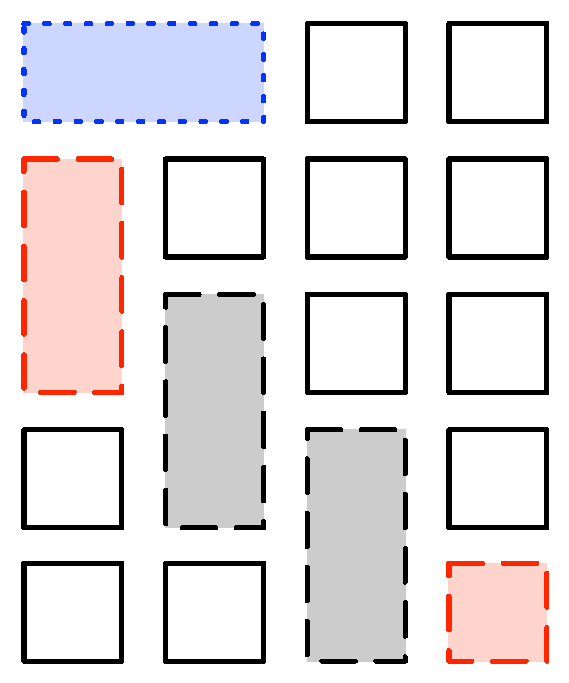
\includegraphics[trim=0 0 0 0,clip,width=1.0\columnwidth]{chapter2/tabletransitive}
\end{minipage}}
\subfloat[\textbf{Textual encoding of input tree.}]{\label{fig:tabletransitive:html}
\begin{minipage}{0.5\columnwidth}\centering
\usebox{\tabletransitivebox}
\end{minipage}
}
\caption{\textbf{Document layout screenshots.}}
\label{fig:docrenderings}
\end{figure}

\subsubsection{Dynamic data structure.}
Figure~\ref{fig:docrenderings} illustrates why the mapping from table cells to table column is dynamically computed. The placement of a cell is complicated by preceding cells that span multiple rows ("rowspan=n") and columns ("colspan=n"). Ultimately, the cell must be placed in the first column such that an earlier cell in a top-down, left-to-right ordering does not overlap it. The figure shows two important cases. First, the second cell of the first row is placed in the third column because its left sibling spans two rows: a cell's column is a function of the \code{rowSpan} attributes of its siblings to the left.  The second case is shown for the bottom right cell. Even though it is the third cell of its row in the parse tree, it is not placed in the third column. The reason is that the red dashed rectangular cell in the second row transitively impacts the placement of the cells after it. The \code{colSpan} attributes of cells in rows above a cell further determine its column.

Our specification computes the column assignment as a loop over the rows. For each row, it computes what columns its cells are placed in as a function of the list of columns that are still occupied by preceding cells. The next row is given the columns that are occupied after adding cells on the current row, etc. Our specification of this behavior is interesting in that it is just calls to functional list manipulation methods written in our host language:
\begin{lstlisting}
class TableBox
  ...
  loop rows {
    rows.colAssignment := 
      fold 
        emptyColumnList(colCount) 
        .. 
        columnsAppendRow(
          rows$-.colAssignment, 
          rows$i.cells, 
          rows$i.rowNum);
\end{lstlisting}
The \code{columnsAppendRow} function computes the column position during placement, so subsequent reads can look it up through another list manipulation function.





\newsavebox{\tabledyna}
\begin{lrbox}{\tabledyna}% Store first listing
\begin{lstlisting}[language=C++,morekeywords={spawn,join,reverse,parallel_for}]
Schedule {
  Col.childs[i].relX <- Col.cellsready
  Col.childs[i].absX <- Col.cellsready
\end{lstlisting}
\end{lrbox}

\newsavebox{\tabledynb}
\begin{lrbox}{\tabledynb}% Store first listing
\begin{lstlisting}[language=C++,morekeywords={spawn,join,reverse,parallel_for}]
schedule { 
  asserta(assignment(col, self, childs_relx_step, self, cellsready)),
  asserta(assignment(col, self, childs_absx_step, self, cellsready))
\end{lstlisting}
\end{lrbox}


\begin{figure}
\subfloat[\textbf{Surface Syntax} (Proposed)]{\label{fig:tabledyndep:clean}
\begin{minipage}{0.5\columnwidth}\centering
\usebox{\tabledyna}
\end{minipage}}
\subfloat[\textbf{Low-level constraint}]{\label{fig:tabledyndep:raw}
\begin{minipage}{0.5\columnwidth}\centering
\usebox{\tabledynb}
\end{minipage}}
\caption{\textbf{Specifying dynamic dependencies.}}
\label{fig:tabledyndep}
\end{figure}

A column computes the x coordinates for each cell, but column cells are not known before the last \code{columnsAppendRow}() call. To ensure a column computes over its cells after the mapping occurs, we explicitly declare the dynamic data dependency in the specification. First, the grid is stored in an attribute, so we simply propagate the grid to all the table nodes as an attribute (\code{cellsready}). We then state the implicit data dependency (Figure~\ref{fig:tabledyndep}. The scheduler now knows to run column computations over cells only after the \code{cellsready} is computed. Currently, we directly specify the constraints by enabling low-level schedule constraints (Figure~\ref{fig:tabledyndep:raw} and Section~[[[???]]), which might be directly generated from surface syntax (Figure~\ref{fig:tabledyndep:clean}).

\subsubsection{Computing over a DAG}
Computing over a table means computing over a DAG, not a tree: a cell has both a row and a column as its parents. This impacted both our runtime and our specification strategy. Demonstrating the flexibility of attribute grammars, we did not have to modify the scheduler nor the code generator. Instead, we modified the runtime and the specification.

We modified the runtime to generalize an important invariant from tree traversals to DAG traversals. In a top down traversal of a tree, a node's parent is visited before the node itself. A valid implementation for trees is depth first. However, consider a depth first traversal of a table's parse tree:
\begin{lstlisting}
<table>
  <row>
    <cell></cell> 
  </row>
  <column></column
</table>
\end{lstlisting}
The depth-first traversal would visit the table, the row, the cell, and then the column. The cell is visited before its parent column! 

Our modification was simple: we edited the runtime to visit the nodes of a table with a breadth first traversal. We kept the overall document traversal as depth first for performance reasons. Declarative schedule constraints would also support picking a breadth-first traversal (Section~\ref{???}).

We also modified the specification to pass our attribute grammar static checker. The changes enables relaxing the scheduler's obligation to guarantee that visiting a cell's parent row and column would set all the attributes needed by the cell (unambiguous) and without conflicting with each other. For example, a column defines the \code{relX} attribute of its child cell, and a row, its \code{relY}. By default, our checker would rightfully reject such a specification because, if a cell has only one parent, only one of those attributes would be set.

We extended the specification language for instructing the scheduler that external code defines certain attributes:
\begin{lstlisting}
class Col : ColI {
  phantom {
    childs.relY;
    childs.absY;
...
class Row : RowI {
  phantom {
    childs.relX;
    childs.absX;
...
\end{lstlisting}
The scheduler now assumes that the external code provides definitions for a column's \code{childs.relY} and \code{childs.absY} and a row's \code{childs.relX} and \code{childs.absX}. Unimportant to the synthesizer, the definitions just happen to come from elsewhere in the same specification, such as class Row defining the phantom attributes not set by Column. %If we wanted to further verify our specification, we could further specify that the assignments of a row and a column to a cell are disjoint sets that, together, hold the assignments needed for a cell, but this is unnecessary for code generation. 

\subsubsection{Non-linear constraints}
The table specification defines a dynamically determined number of loops over a table's column to determine column widths. Such dynamism is beyond the pure static attribute grammar formalism, but our foreign function interface sufficed while still allowing overall specification and scheduling through attribute grammars.

\subsection{Flow-based: CSS Box Model}
Document layout languages generally feature a \emph{flow-based} layout model where the position of one element is largely a function of the previous one. For example, line wrapping places one word after another in a paragraph, and a column will stack one paragraph after another. However, ambiguity quickly arises once constraints are added to such systems. We found that, before being able to address our interest in parallelizing the CSS language, that creating a functional specification of it was already a challenge to itself.  This section focuses on the ability to express the CSS specification, and defers discussion of functional correctness (Chapter~??) and safe parallelization (Chapter~??).

Challenging specification, the CSS standard provides only a few explicit formulas such as  \code{min(max(intrinsMinWidth,maxWidth),intrinsPrefWidth)} for the shrink-to-fit calculation. It generally does not fully define the intrinsic dimensions to plug into the formula. We incorporated what we found, and for the rest, spent significant time reengineering the semantics by examining the standard and experimenting with existing browsers. While it is unclear how to evaluate faithfulness, we encoded enough features to render a resemblance of the Wikipedia main page (Figure~\ref{fig:rendering:css}) and a popular blog.

Our attribute grammar describes the layout solving features of the informally written CSS 2.1 standard. It also includes automatic table layout, which was only more completely defined in later CSS standards. It does not include preprocessing steps, such as the CSS cascade that annotates the HTML tree with attributes, nor anonymous content generation, which normalizes the annotated tree to guarantee that spans of sibling nodes are homogeneous. The former is largely a combination of a simple extension to regular expressions and prioritization constraints. We found we could include parts of the cascade in our approach, such as handling units, and thus do.  Normalization is a bottom-up tree rewriting pass, and an implementation optimization avoids performing it before layout and instead makes it an on-demand part of layout solving. We primarily focus in the core box model: normal flow (blocks and inlines), out of flow (relative and absolute positioning, floats), and borders, padding, and margins.

Our specification largely follows the style of the above grammars. Part of the intuition for the feasibility of specifying CSS in this way is that CSS was designed with restrictions that avoid requiring slow evaluation with techniques such as iterative constraint solving. In our encoding, each CSS display type is represented by one or more classes in our system. CSS's normalization algorithm largely leads to our set of interfaces, such as grouping the \code{inline} and \code{inline-block} display types under interface \code{inline}. We make heavy use of traits and interfaces, which compromise 23\% and 32\% of the code, respectively. The automatic table layout algorithm was an extension of the above techniques. Finally, similar to the issue with table cells having two parents, a row and a column, out of flow elements also required encodings to support DAG behavior. 

Several differences distinguish our experience with specifying CSS layout from the other case studies. Many features were difficult to specify because of many cases or cross-cutting in their semantics. Discussed in Chapter~\cite{??}, we rely upon automatic checking to assist development, and discussed in Chapter~\cite{??}, we specify schedule sketches to improve compiler speed and more quickly experiment with parallelization schemes. To further simplify development, we wrote several increasingly large specifications and manually integrated them.

One particularly challenging feature to disentangle relates to ambiguity. CSS  solves seemingly inconsistent input constraints instead of returning an error. For example, if \hlang was extended to support input heights on intermediate nodes, the following conflict would require a graceful interpretation rather than refusing to render:
\begin{lstlisting}
<hbox height="5">
  <hbox height="500"></hbox>
</hbox>
\end{lstlisting}
By the original attribute grammar, the outer \code{<hbox>} should be the size of the biggest child, which would be 500. However, that conflicts with the input constraint of the outer box only being 5 tall. Our CSS grammar inspects for the presence of input attributes and prioritizes them. The analogous resolution for the \hlang example is the following:
\begin{lstlisting}
loop children { 
  h := 
    fold (maybeReady(height) ? maybeValue(height) : 0)
    ..
    maybeReady(height) ? maybeValue(height) : max($-.h, child.h) 
}
\end{lstlisting}
The grammar uses "5" and "500" because they were explicitly specified instead of solving for them.  

We found other features to be difficult because they purposefully stray from the direct mathematical interpretation. For example, CSS supports input constraints where a node's width is defined as a proportion of its parent's. If we na\"{i}vely extended \hlang with such a feature, evaluation of the following layout would lead to a degenerate solution:
\begin{lstlisting}
<hbox>
  <hbox width="50%">
     <hbox w="20"></hbox>
  </hbox>
</hbox>
\end{lstlisting}
The root node shrinks to fit the middle node, but the middle node must be 50\% of the parent. Direct interpretation leads to a solution of 0 for both widths, but CSS instead leaves the result up to the layout engine implementation. The first reason is that the result looks unappealing: the containers of the leaf node do not appear. The second reason is that, while iterative solvers may avoid some such situations, but at the expense of performance. Implementations instead use non-iterative heuristics, but as seen with tables, implementors struggle to understand them.

In summary, our attribute grammar formalism was sufficiently flexible to specify a non-trivial subset of the widely used CSS language. We encountered several key difficulties, and discuss those relating to correctness, safe and effective parallelization, and compiler speed in Chapters~\ref{???} and~\ref{???}.


\section{Related Work}
\begin{itemize}
\item loose formalisms: browser impl (C++), d3 (JavaScript), latex formulas (ML)
\item restricted formalisms: cassowary and hp, UREs
\item AGs: html tables
\end{itemize}



 %ag / extension
\chapter{A Static Scheduling Language for Parallel Tree Traversals}
\label{chap:3}

We now introduce a static scheduling language for parallel computations over a tree such as those seen in layout. A compiler takes an attribute grammar (the functional specification) and its schedule and outputs an implement, i.e., a layout engine. For now, we ignore the source of the schedule. Beyond presenting the language and compilation strategy, we show how to verify functional and behavioral (parallel) correctness, introduce the first parallel schedule for a large subset of CSS, and show how, on GPU tree computations, memory may be dynamically allocated quite efficiently.

The goal of our language for traversals over trees is to benefit from high-performance computing techniques  commonly used for stencils over grids. Common for physical modeling, a stencil computation is one where a kernel only reads and writes to a limited set of nodes, there are many kernels, and the data dependencies between kernels lead to traversal patterns such as a wavefront. Many variants of stencils exist. The enthusiasm for them stems from programmers or stencil compilers being able to exploit knowledge of their structure to effectively optimize for use of cache lines, memory, parallel processors, and other resources. Similar techniques are known for trees, and the next chapter introduces additional ones.

Our first challenge in this chapter is to restrict the scheduling language enough to facilitate optimization while still providing the flexibility for expressing  document layout and data visualization workloads. Finding parallelism in CSS is already novel,  so being further able to optimize it with techniques associated with small formulas for physical models is surprising. We found that, while layout computations have too many data dependencies to be solved with one simple tree traversal, sequences of 3--5 traversals often suffice for data visualizations and 9 for CSS. Our scheduling language therefore consists of traversal patterns, such as parallel top down (\emph{preorder}) traversal of the tree, and ways of combining them, such as in a sequence. One especially representative case study of matching restrictions with flexibility was in our study of  visualizations: dynamic memory allocation on a GPU is generally a bottleneck, but we used a sequence of tree traversals for parallel allocation of render buffers for each node.

Another artifact of layout specifications being magnitudes bigger than stencil formulas is that the correctness concerns change. For stencil computations, the verification challenge lies more in correctly optimizing the implementation of a traversal schedule. Layout computations encounter a challenge before that point: the size of the functional specification and the ensuing tangle of data dependencies require ensuring  that the parallel schedule itself is safe to implement. We use a variant of existing static dependency analyses of attribute grammars to verify that the schedule is race-free. 


The dependencies that complicate reasoning about correctness of parallel code actually also complicate sequential code. Our use of static analysis for the attribute grammars leads to an important result for layout languages: we show how to statically verify three important properties about them.  
\begin{itemize}
\item \textbf{Totality} The layout language defines a solution for every syntactically well-formed input tree; it is unambiguous. 
\item \textbf{Determinism} As discussed  in the previous paragraph, parallelization is safe.
\item \textbf{Linearity (Single Assignment)} Every attribute is assigned to exactly once. Layout languages often perform \emph{reflow} to iteratively solve constraints or incremental computation, so this property bounds the need for it. 
\end{itemize}
The first property demonstrates the ability to reason about \emph{functional correctness} and the last two about \emph{behavioral correctness}. Put together, we verify that a language is unambiguous, supports parallelization, and with bounded asymptotic complexity.  

\section{Language of Static Schedules}
%Our approach builds upon the ideas of multipass attribute grammars and statically ordered attribute grammars~\cite{oag}. Before showing our technique, we review how to use these ideas on how to more efficiently evaluate attribute grammars than the na\"{i}ve dynamic approach of Chapter~\ref{chap:2}. Furthermore, we review how they enable proving properties about the attribute grammars such as unambiguity, and (inefficient) parallelization strategies. 

This section focuses on defining our full language of traversal schedules. It is the input for our code generators. Programmers either do not specify the schedule in practice due to our automation support, or use the \emph{sketching} extension (Section~\ref{sec:holes}) for more succinct partial specification.

Statically scheduled evaluation departs from the dynamic evaluation strategy of Chapter~\ref{chap:2}. Static scheduling solves the performance problem of dynamic evaluation repeatedly manipulating the data dependencies of every attribute at runtime. For example, what would be a direct sequence of arithmetic statements in a static language becomes an interleaving of graph manipulations and arithmetic with the dynamic evaluator. The runtime scheduling overhead for evaluating all the statement is (at least) linear in the size of the data dependency graph. 

Instead, a schedule statically specifies most of the scheduling decisions.  It specifies a sequence of tree traversals and the order of statements to use within each traversal. During a traversal at runtime, the order of nodes to traverse is based on the traversal pattern, such as top-down, rather than by inspecting data dependencies. Likewise, the statements to execute for a node are looked up based on the node's type rather than by data dependencies.  Our approach is a more compositional variant of others. Our flexibility requirements led to focusing on the ability to compose different types of traversals, such as by sequencing and nesting.


\newsavebox{\seqtraversals}
\begin{lrbox}{\seqtraversals}% Store first listing
\begin{minipage}{1\columnwidth}
\begin{lstlisting}[mathescape,language=C++,morekeywords={spawn,join}]
void preorder(void (*visit)(Prod &), Prod &p) {
  visit(p);
  for (Prod rhs in p) 
    preorder(visit, rhs);
}
void postorder(void (*visit)(Prod &), Prod &p) {
  for (Prod rhs in p) 
    postorder(visit, rhs);
  visit(p);
}
void recursive(void (*visit)(Prod &, int), Prod &p) {
    int step = 0;
    visit(p, step++);
    for (Prod rhs in p) {
      recursive(visit, rhs);
      visit(p, step++); //repeat visit to p
    }
}
\end{lstlisting}
\end{minipage}
\end{lrbox}

\newsavebox{\seqtraversalsequence}
\begin{lrbox}{\seqtraversalsequence}% Store first listing
\begin{minipage}{1\columnwidth}
\begin{lstlisting}[mathescape,language=C++,morekeywords={spawn,join}]
postorder(visit1, start); 
preorder(visit2, start);
\end{lstlisting}
\end{minipage}
\end{lrbox}


\newsavebox{\hboxvisitors}
\begin{lrbox}{\hboxvisitors}% Store first listing
\begin{minipage}{1\columnwidth}
\begin{lstlisting}[mathescape,language=C++]
void visit1 (Prod &p) {
  switch (p.type) {
    case S $\rightarrow$ HBOX:  break;
    case HBOX $\rightarrow$ $\epsilon$:
      HBOX.w = input(); HBOX.h = input(); break;
    case HBOX $\rightarrow$ HBOX$_1$ HBOX$_2$:
      HBOX$_0$.w = HBOX$_1$.w + HBOX$_2$.w;
      HBOX$_0$.h = MAX(HBOX$_1$.h, HBOX$_2$.h);
      break;
  }
}
void visit2 (Prod &p) {
  switch (p.type) {
    case S $\rightarrow$ HBOX:
      HBOX.x = input(); HBOX.y = input(); break;
    case HBOX $\rightarrow$ $\epsilon$: break;
    case HBOX $\rightarrow$ HBOX$_1$ HBOX$_2$:
      HBOX$_1$.x = HBOX$_0$.x;
      HBOX$_2$.x = HBOX$_0$.x + HBOX$_1$.w;
      HBOX$_1$.y = HBOX$_0$.y;
      HBOX$_2$.y = HBOX$_0$.y;
      break;
  }
}
\end{lstlisting}
\end{minipage}
\end{lrbox}




\begin{figure}
\subfloat[\textbf{Sequential sequence of traversals}]{\label{fig:hboxseq:sequence} \usebox{\seqtraversalsequence} } \\
\subfloat[\textbf{Three sequential traversal patterns}]{\label{fig:hboxseq:traversals} \usebox{\seqtraversals} } \\
\subfloat[\textbf{Scheduled and compiled visits for ~\hlang{}.}]{\label{fig:hboxseq:compiled} \usebox{\hboxvisitors} } \\
\caption{\textbf{Sequentially scheduled and compiled layout engine for \hlang{}.}}
\label{fig:hboxseq}
\end{figure}





\subsection{Sequential Schedules}  
\label{subseq:seqscheds}
We start by examining how to specify a safe static schedule for \hlang that respects any possible dynamic dependencies (Figure~\ref{fig:deps:full}).
%Research into statically scheduled sequential attribute grammars revealed a variety of scheduling options. For example, some computations can be solved in one traversal over a tree and therefore merged into a parser, while others require multiple traversals. We focus on several important options and the automated reasoning supported for them.

Figure~\ref{fig:hboxseq} shows a sequential implementation of \hlang decomposed into several pieces. The layout engine solves an input tree over a sequence of two traversals (Figure~\ref{fig:hboxseq:sequence}). The first traverses the tree in postorder, meaning from the leaves up to the root (''bottom-up'') and the second performs are preorder traversal, meaning from the root down to the leaves (''top-down''). Figure~\ref{fig:hboxseq:traversals} provides a sample implementation of generic traversal code. During a during traversal, each node is \emph{visited} exactly once in order to compute the attributes whose dependencies have been satisfied. Figure~\ref{fig:hboxseq:compiled} shows that the first pass computes widths and heights and the second pass computes the x and y positions.

The example follows a static schedule rather than manipulating a dynamic data dependency graph. The sequence of traversal invocations and the code used for the different cases for each traversal's visitor determine the schedule. Each traversal now only performs dynamic scheduling in the sense of maintaining a stack for recurring down the tree, which is a cost proportional to the number of nodes rather than the size of the dynamic dependency graph between attributes. In practice (Chapter~\ref{chap:6}), our compiler and runtime optimizations even eliminate the example's implicit use of a call stack.


The decompose the schedule into several types of policy fragments. First, the schedules involves a \emph{sequence} of  \emph{two different types} of traversals:
\begin{lstlisting}
      postorder(visit1, start); preorder(visit2, start)
\end{lstlisting}
Just one bottom-up traversal cannot compute all the attributes, such as all the x and y attributes that flow downwards (Figure~\ref{fig:deps:full}), so the schedule may require multiple types of traversals and in a careful order.  Furthermore, within a traversal, the schedule specifies different orders of statements for different types of nodes. Consider the following fragment:
\begin{lstlisting}
      HBOX$_1$.x = HBOX$_0$.x;
      HBOX$_2$.x = HBOX$_0$.x + HBOX$_1$.w;
\end{lstlisting}
The schedule specifies that \code{HBOX}$_2$\code{.x} can (and should) be immediately evaluated after \code{HBOX}$_1$\code{.x} without fear of unsatisfied data dependencies for any of its right-hand side terms. In summary, we see three parts to a schedule: the staging of traversals, the node visit order for every individual traversal, and the statement order for different types of nodes within a specific traversal.

We abstracted the three aspects of a schedule into a scheduling language (Figure~\ref{fig:hboxparallel}). For example, the schedule for the above computation would be appear as:
\begin{lstlisting}[mathescape,morekeywords={preorder,postorder}]
postorder
  HBOX$_0$ $\rightarrow$ HBOX$_1$ HBOX$_2$ { HBOX$_0$.w HBOX$_0$.h }
  HBOX $\rightarrow$ $\epsilon$ { HBOX.w HBOX.h }
;
preorder
  S $\rightarrow$ HBOX { HBOX.x HBOX.y }
  HBOX$_0$ $\rightarrow$ HBOX$_1$ HBOX$_2$ 
    { HBOX$_1$.x HBOX$_2$.x HBOX$_1$.y HBOX$_2$.y }
\end{lstlisting}
It specifies a sequence ('';'') of two traversals of node visit order \code{postorder} and \code{preorder}. For each type of node visited within a traversal, the schedule specifies the sequential sequence of attributes to evaluate. We note that, due to the desugaring of our class system in Section~\ref{sec:desugaring}, the dispatches in the above examples are based on grammar productions in the desugared representation. In terms of the fronted language, the dispatches are based on node class.


Generally, a single attribute grammar may be schedule in many ways. For example, the width and height computations share no dependencies, so the first postorder traversal might be partitioned into two postorder traversals:
\begin{lstlisting}[mathescape,morekeywords={preorder,postorder}]
postorder
  HBOX$_0$ $\rightarrow$ HBOX$_1$ HBOX$_2$ { HBOX$_0$.w }
  HBOX $\rightarrow$ $\epsilon$ { HBOX.w }
;
postorder
  HBOX$_0$ $\rightarrow$ HBOX$_1$ HBOX$_2$ { HBOX$_0$.h }
  HBOX $\rightarrow$ $\epsilon$ { HBOX.h }
;
preorder
  S $\rightarrow$ HBOX { HBOX.x HBOX.y }
  HBOX$_0$ $\rightarrow$ HBOX$_1$ HBOX$_2$ 
    { HBOX$_1$.x HBOX$_2$.x HBOX$_1$.y HBOX$_2$.y }
\end{lstlisting}
Rescheduling in this way may improve performance on small devices with little memory because the schedule cuts the working set size in half for each traversal. Note, however, that the schedule only optimizes execution; it does not change the result of evaluation.


\begin{figure}
\centering
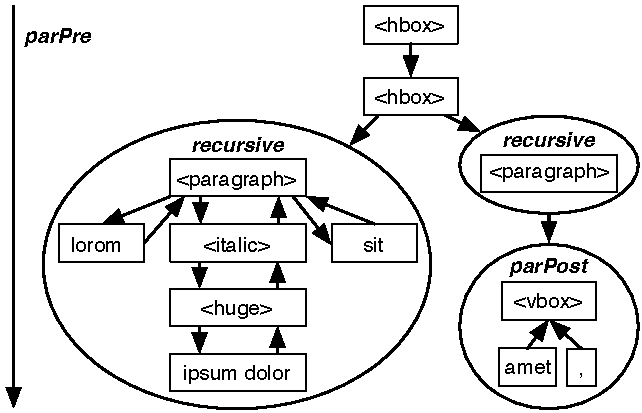
\includegraphics[trim=0 0 0 0,clip,width=0.7\columnwidth]{chapter3/nested}
\caption{\textbf{Nested traversal for line breaking}. The two paragraphs are traversed in parallel as part of a preorder traversal. A sequential recursive traversal places the words within a paragraph. Circles denote nested regions and arrows show data dependencies between nodes and/or regions.}
\label{fig:nested}
\end{figure}

Sequential execution supports a traversal type that can compute more than \code{postorder} or \code{preorder}, which we call a \code{recursive} traversal (Figure~\ref{fig:hboxseq:traversals}). We use a recursive traversal, for example, for line breaking in our document layout case study. Consider inserting line breaks into the following stylized paragraph of XML strings (Figure~\ref{fig:nested}):
%
$$\texttt{lorom <italic><huge>ipsum dolor</huge></italic> sit}$$
%
Due to \texttt{<huge>}, the paragraph may need a line break between ``ipsum'' and ``dolor.''  Identifying the line break position involves visiting the subtree  \texttt{<italic>...</italic>}; the resulting line break position is a data dependency influencing line breaks in the remainder of the text. The sequence of arrows in the big circle of Figure~\ref{fig:nested} show a trace of performing a recursive traversal over the paragraph. The traversal visits a node $n$, then visits $n$'s first child, revisits $n$, and repeats this process for the remaining children before returning to the parent. 

The relationship between \code{recursive} traversals and \code{postorder} and \code{preorder} merits examination. First, a sequence of a preorder traversal followed by a postorder traversal may be merged into one recursive traversals. Traversing a tree induces overhead costs, so such fusion may be beneficial. The reverse  relationship is not true, however. As happens with the case of line breaking, long-running sequential dependencies may prevent splitting a recursive traversal into a preorder and postorder traversal. These dependencies arise because the the same node is visited multiple times in a traversal: once before a child subtree is traversed and again after. The result of computing over one subtree may therefore be used to compute another, which supports long-running sequential dependencies. 


\newsavebox{\decomplang}
\begin{lrbox}{\decomplang}% Store first listing
\begin{minipage}{1\columnwidth}
\renewcommand{\litleft}{\bfseries}
\renewcommand{\ulitleft}{\bfseries}
\renewcommand{\superscript}[1]{\ensuremath{^{\textrm{#1}}}}
\renewcommand{\subscript}[1]{\ensuremath{_{\textrm{\uppercase{#1}}}}}
\renewcommand{\syntleft}{\normalfont\itshape\texttt{<}}
\renewcommand{\syntright}{\texttt{>}}
\begin{grammar}
<Sched> \deriv{} <Sched> ; <Sched>  ~ | ~ <Sched> $\vert\vert$ <Sched>  ~|~ <Trav>

<Trav> \deriv{} <TravAtomic> <Visit>*\{(<TravAtomic> $\mapsto$ <Visit>*)*\}?

<TravAtomic>  \deriv{} "preorder" ~ | ~ "postorder" ~ | ~ "parPre"  ~ | ~  "parPost"  ~ | ~  "recursive" ~ 

<Visit> \deriv{} <Prod>  \{ <Step>* \}

<Step> \deriv{} \emph{attrib} ~ | ~ "recur" \emph{v}
\end{grammar}
%<Sched, Trav, Visit, Step> \deriv{} \ldots ~ | ~ $\hole$        
\end{minipage}
\end{lrbox}


\newsavebox{\hboxdecomp}
\begin{lrbox}{\hboxdecomp}% Store first listing
\begin{minipage}{1\columnwidth}
\begin{lstlisting}[mathescape,morekeywords={parPre,parPost}]
parPost
  HBOX$_0$ $\rightarrow$ HBOX$_1$ HBOX$_2$ { HBOX$_0$.w HBOX$_0$.h }
  HBOX $\rightarrow$ $\epsilon$ { HBOX.w HBOX.h }
;
parPre
  S $\rightarrow$ HBOX { HBOX.x HBOX.y }
  HBOX$_0$ $\rightarrow$ HBOX$_1$ HBOX$_2$ 
    { HBOX$_1$.x HBOX$_2$.x HBOX$_1$.y HBOX$_2$.y }
\end{lstlisting}
\end{minipage}
\end{lrbox}

\newsavebox{\traversals}
\begin{lrbox}{\traversals}% Store first listing
\begin{minipage}{1\columnwidth}
\begin{lstlisting}[mathescape,language=C++,morekeywords={spawn,join}]
void parPre(void (*visit)(Prod &), Prod &p) {
  visit(p);
  for (Prod rhs in p) 
    spawn parPre(visit, rhs);
  join;
}
void parPost(void (*visit)(Prod &), Prod &p) {
  for (Prod rhs in p) 
    spawn parPost(visit, rhs);
  join;
  visit(p);
}
\end{lstlisting}
\end{minipage}
\end{lrbox}

\newsavebox{\hboxparvisitors}
\begin{lrbox}{\hboxparvisitors}% Store first listing
\begin{minipage}{1\columnwidth}
\begin{lstlisting}[mathescape,language=C++]
parPost(visit1, start); parPre(visit2, start);
\end{lstlisting}
\end{minipage}
\end{lrbox}


\begin{figure}
\subfloat[\textbf{One explicit parallel schedule for ~\hlang{}.}]{\label{fig:hboxparallel:schedule} \usebox{\hboxdecomp} } \\
\subfloat[\textbf{Na\"{\i}ve traversal implementations} with Cilk's~\cite{cilk} \sched{spawn} and \sched{join}.]{\label{fig:hboxparallel:traversals} \usebox{\traversals} } \\
\subfloat[\textbf{Scheduled and compiled layout engine for ~\hlang{}.}]{\label{fig:hboxparallel:compiled} \usebox{\hboxparvisitors} } \\
\subfloat[\textbf{Language of schedules} (without holes) ]{\label{fig:hboxparallel:decomplang} \usebox{\decomplang} }
\caption{\textbf{Scheduled and compiled layout engine for \hlang{}.}}
\label{fig:hboxparallel}
\end{figure}




\begin{figure}
\subfloat[First traversal: parallel postorder]{\label{fig:depsparallel:postorder}
\begin{minipage}{0.5\columnwidth}\centering
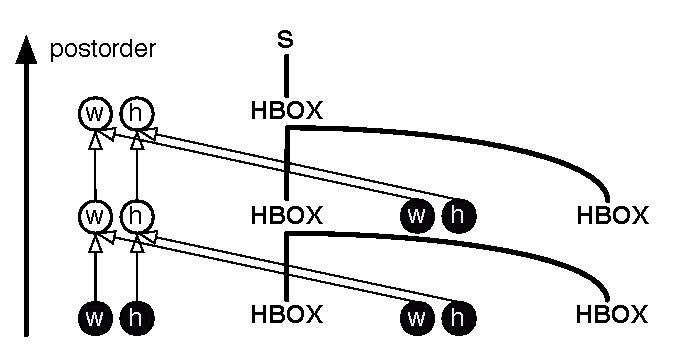
\includegraphics[trim=0 0 0 0,clip,width=1.0\columnwidth]{chapter3/depspostorder}
\end{minipage}}
\subfloat[Second traversal: parallel preorder.]{\label{fig:depsparallel:preorder}
\begin{minipage}{0.5\columnwidth}\centering
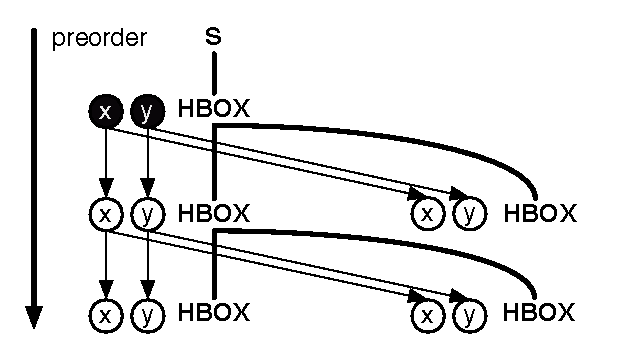
\includegraphics[trim=0 0 0 0,clip,width=1.0\columnwidth]{chapter3/depspreorder}
\end{minipage}}
\caption{\textbf{Parallel Traversal}. Shown for constraint tree  in Figure~ZZZ~(a). Circles denote attributes, with black circles denoting attributes with resolved dependencies such as \sched{input()}s. Thin lines show data dependencies and thick lines show production derivations. First diagram shows dependencies followed by first traversal, and second for the following traversal.}
\label{fig:depsparallel}
\end{figure}


\subsection{Parallel Schedules: Same Traversal}
A schedule exposes structured parallelism both within a traversal and across them. 

For an example of parallelism within a traversal, the first postorder traversal for \hlang features latent parallelism. The widths and heights for one subtree can be computed independently of the widths and heights of another distinct subtree. Figure~\ref{fig:depsparallel:postorder} shows an example where different (logical) threads may compute on the leaf nodes and implicit barriers force a join at every intermediate node. Likewise, the second traversal (Figure~\ref{fig:depsparallel:preorder}) may be changed to a parallel preorder traversal where ever intermediate node acts as a logical fork. Figure~\ref{fig:hboxparallel:traversals} depicts na\"{i}ve parallel implementations using Cilk's~\cite{??} \code{spawn} and \code{join} primitives. We formulate the schedule by changing the specification from \code{postorder} and \code{preorder} to \code{parPost} and \code{parPre} (Figure~\ref{fig:hboxparallel:schedule}).


Our \emph{nested} traversal feature supports exploiting parallelism within a traversal even if some nodes require sequential evaluation.  With it, the tree is partitioned into an outer region and disjoint inner regions.  The outer and inner regions are evaluated with different traversals, and both may exploit parallelism.  We can think of the inner regions as macro-nodes that are evaluated in full (with their particular traversal type) when the outer traversal encounters them.  

To motivate the need for nested traversals, we revisit line breaking.  Even though line breaking of a single paragraph is sequential, distinct paragraphs of text can be handled in parallel.  To avoid locally sequential computations from forcing the entire tree traversal to be sequential, we allow the outer region to be parallel, while each paragraph forms an inner region that is handled with the sequential recursive traversal. Figure~\ref{fig:nested} shows how parallel evaluation may be used to compute across different \sched{recursive} paragraphs. Likewise, it shows a hypothetical \code{VBox} subtree that uses parallel postorder evaluation for traversing its subtree as soon as the outer parallel preorder traversal reaches it.

%A nested traversal supports parallelism. First, the outer traversal may itself be parallel, such as the two paragraphs in Figure~\ref{fig:nested} being evaluated concurrently as part of an overall preorder traversal. Second, each macro-node may itself be evaluated with a parallel traversal internally whenever the outer traversal reaches it. For example, parallel evaluation may be used within the preorder and postorder macro-nodes in Figure~\ref{fig:nested}.

To partition a tree into regions, the schedule maps each grammar production (and thus each node of the tree) to a traversal type in the synthesized schedule.  A subtree composed from nodes of the same traversal types form an inner region.  For example, a nested traversal of paragraphs with sequential traversals of nested text subtrees is described as follows: 

\begin{lstlisting}[mathescape,morekeywords={parPre,parPost,nested,recursive,recur}]
parPre 
  P $\rightarrow$ W { W.relativeX }
  { recursive $\mapsto$   
      W$_0$ $\rightarrow$ W$_1$ W$_2$ {
        W$_1$.relativeX recur W$_1$ 
        W$_2$.relativeX recur W$_2$ } }
\end{lstlisting}


\subsection{Parallel Schedules: Across Travesals}
We may exploit parallelism across traversals as well. For example, just as we created a different but functionally equivalent sequential schedule for \hlang, we can do the same manipulation to yield a new parallel schedule:

\begin{minipage}{1\columnwidth}
\begin{lstlisting}[mathescape,morekeywords={parPre,parPost}]
(   parPost
     HBOX$_0$ $\rightarrow$ HBOX$_1$ HBOX$_2$ { HBOX$_0$.w }
     HBOX $\rightarrow$ $\epsilon$ { HBOX.w }  
   $||$  
    parPost
     HBOX$_0$ $\rightarrow$ HBOX$_1$ HBOX$_2$ { HBOX$_0$.h }
     HBOX $\rightarrow$ $\epsilon$ { HBOX.h })
; parPre $\ldots$ $\emph{/* same as before */}$
\end{lstlisting}
\end{minipage}
The ``$||$'' construct specifies that one traversal may be run concurrently with another. Neither traversal traversal depends on attributes written by the other, so the parallelizaton is safe. Even if we cannot exploit parallelism within a traversal, using ``$||$'' enables us to exploit parallel across them. 









\subsection{Compilation}
Compilation only requires an attribute grammar and the schedule. The traversal staging \code{postorder _ ; preorder _} directly translates to the executable fragment in Figure~\ref{fig:hboxseq:sequence}. Likewise, the mapping from traversal productions to statement sequences, such as \code{HBOX} $\rightarrow \epsilon$ \{ \code{HBOX.w HBOX.h} \}, directly translate to the visit functions of Figure~\ref{fig:hboxseq:compiled}. The translation matches an attribute in the schedule with the lefthand side attribute of an equation in the attribute grammar and outputs the full assignment statement in its place. 

Our code generation pipeline is further complicated but conceptually similar. The schedule is combined with the attribute grammar to form an intermediate representation, and different code generators target different backends, such as JavaScript, OpenCL, and C++. Furthermore, some of the reductions of Section~\ref{sec:desguaring} require augmenting or rewriting the intermediate representation, such as reinserting loops that were unrolled during scheduling (Section~\ref{???}). Our end-to-end compiler design is slightly different due to the synthesis algorithm (Chapter~\ref{chap:4})  and schedule autotuning (Section~\ref{sec:schedtuning}), but code generation for a schedule follows a more conventional process.


\section{Automatically Staging Memory Allocation for SIMD Rendering}
\newsavebox{\stagedAllocFull}
\begin{lrbox}{\stagedAllocFull}% Store first listing
\begin{lstlisting}[mathescape]
float *drawCircle (float x, float y, float radius) {
  float *buffer = malloc( (2 * sizeof(float) ) * round(radius))
  for (int i = 0; i < round(radius); i++) {
    buffer[2 * i] = x + cos(i * PI/radius);
    buffer[2 * i + i] = y + sin(i * PI/radius);
  }
  return buffer;
}
\end{lstlisting}
\end{lrbox}

\newsavebox{\stagedAllocAlloc}
\begin{lrbox}{\stagedAllocAlloc}% Store first listing
\begin{lstlisting}[mathescape]
int allocCircle (float x, float y, float radius) {
  return round(radius);
}
\end{lstlisting}
\end{lrbox}


\newsavebox{\stagedAllocRender}
\begin{lrbox}{\stagedAllocRender}% Store first listing
\begin{lstlisting}[mathescape]
int fillCircle(float x, float y, float radius, float *buffer) {
  for (int i = 0; i < round(radius); i++) {
    buffer[2 * i] = x + cos(i * PI/radius);
    buffer[2 * i + i] = y + sin(i * PI/radius);
  }	
  return 0;
}
\end{lstlisting}
\end{lrbox}


\begin{figure}
\subfloat[\textbf{Na\i{v}e drawing primitive .}]{\label{fig:stagedalloc:original} \usebox{\stagedAllocFull} }  \\
\subfloat[\textbf{Allocation phase of drawing}.]{\label{fig:stagedalloc:alloc} \usebox{\stagedAllocAlloc} } \\
\subfloat[\textbf{Tessellation phase of drawing}.]{\label{fig:stagedalloc:use} \usebox{\stagedAllocRender} } 
\caption{\textbf{Partitioning of a library function that uses dynamic memory allocation into parallelizable stages.}}
\label{fig:stagedalloc}
\end{figure}


\newsavebox{\twocirclesOrig}
\begin{lrbox}{\twocirclesOrig}% Store first listing
\begin{lstlisting}[mathescape]
CBOX $\rightarrow$ BOX$_1$ BOX$_2$
{
  ...
  CBOX.render = 
    drawCircle(CBOX.x, CBOX.y, CBOX.radius)
      + drawCircle(CBOX.x + 10, CBOX.y + 10, CBOX.radius * 0.5);
}
\end{lstlisting}
\end{lrbox}

\newsavebox{\twocirclesExpanded}
\begin{lrbox}{\twocirclesExpanded}% Store first listing
\begin{lstlisting}[mathescape]
CBOX $\rightarrow$ BOX$_1$ BOX$_2$
{
  ...
  CBOX.sizeSelf = 
    allocCircle(CBOX.x, CBOX.y, CBOX.radius)
      + allocCircle(CBOX.x + 10, CBOX.y + 10, CBOX.radius * 0.5);
  CBOX.size = CBOX.sizeSelf +BOX$_1$.size + BOX$_2$.size;
  BOX$_1$.buffer = CBOX.buffer + CBOX.sizeSelf;
  BOX$_2$.buffer = BOX$_1$.buffer + BOX$_1$.size;
  CBOX.render = 
    fillCircle(CBOX.x, CBOX.y, CBOX.radius, CBOX.buffer)
      + fillCircle(CBOX.x + 10, CBOX.y + 10, CBOX.radius * 0.5,
            CBOX.buffer + allocCircle(CBOX.x, CBOX.y, CBOX.radius));
}
\end{lstlisting}
\end{lrbox}

\newsavebox{\twocirclesMacro}
\begin{lrbox}{\twocirclesMacro}% Store first listing
\begin{lstlisting}[mathescape]
CBOX $\rightarrow$ BOX$_1$ BOX$_2$
{
  ...
  CBOX.render = 
      @Circle(CBOX.x, CBOX.y, CBOX.radius)
      + @Circle(CBOX.x + 10, CBOX.y + 10, CBOX.radius * 0.5);
}
\end{lstlisting}
\end{lrbox}




\begin{figure}
\subfloat[\textbf{Call into inefficient library.}]{\label{fig:stagedallocClient:original} \usebox{\twocirclesOrig} }  \\
\subfloat[\textbf{Macro-expanded calls into staged library}.]{\label{fig:stagedallocClient:expanded} \usebox{\twocirclesExpanded} }  \\
\subfloat[\textbf{Sugared calls into staged library}.]{\label{fig:stagedallocClient:macro} \usebox{\twocirclesMacro} } 
\caption{\textbf{Use of dynamic memory allocation in a grammar for rendering two circles.}}
\label{fig:stagedallocClient}
\end{figure}

\begin{figure}
\centering
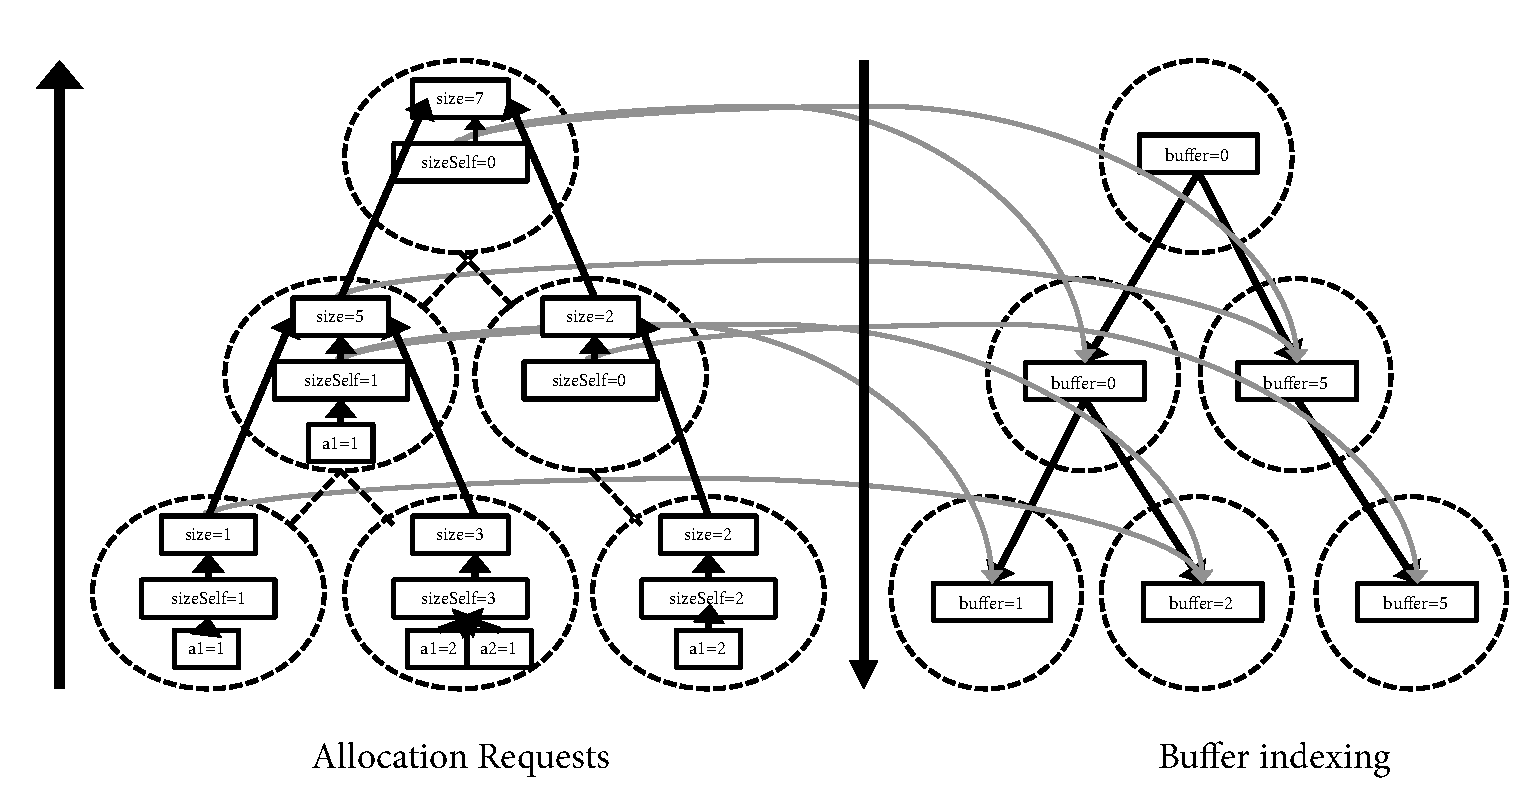
\includegraphics[trim=0 0 0 0,clip,width=1.0\columnwidth]{chapter6/macro}
\caption{\textbf{Staged parallel memory allocation as two tree traversals.} First pass is parallel bottom-up traversal computing the sum of allocation requests and the second pass is a parallel top-down traversal computing buffer indices. Lines with arrows indicate dynamic data dependencies.}
\label{fig:renderingtraversal}
\end{figure}


\subsection{Problem}
The static language of traversals is restricted, but we find that it can express important cases of typically more dynamic constructs. Prominent in our case studies, dynamic memory allocation provides significant flexibility for a language, but it is unclear how to perform it on a GPU without significant performance penalties. Our insight is that the memory allocation may be staged with parallel traversals by using a variant of prefix sum node labeling. One pass gathers  memory requests, a bulk allocation for the total amount is made, and then a scatter pass provides each node with a contiguous memory segment of it. We found manipulating memory addresses in this way to be error-prone, so we created two complementary automation techniques. First, we use our synthesizer to automatically schedule parallel memory allocation. Second, we syntactically hide the use of our optimization through a macro that automatically expands into staged dynamic memory allocation and consumption calls.

For example, we found parallel dynamic memory allocation to simplify the transition between layout and rendering. All nodes that render a circle will call some form of \code{drawCircle} in Figure~\ref{fig:stagedalloc:original}. Depending on the size of the circle, which is computed as part of the layout traversals, a different amount of memory will be allocated. Once the memory is allocated, vertices will be filled in with the correct position. The rendering engine will then connect the vertices with lines and paint them to the screen. The processing of converting the abstract shape into renderable vertices is known as tessellation. We want our system to tesselate the display objects for each node in parallel.




\subsection{Staged Parallel Memory Allocation}
We stage the use of dynamic memory into four logical phases: 
\begin{enumerate}
\item Parallel request (bottom-up tree traversal to gather )
\item Physical memory allocation
\item Parallel response (top-down tree traversal to scatter)
\item Computations that consume dynamic memory (normal parallel tree traversals)
\end{enumerate}
 The staging allows us to parallelize the request and response stages. We reuse the parallel tree traversals for them, as well as for the actual consumption. The actual allocation of physical memory in stage 2 is fast because it is a single call. Figure~\ref{fig:renderingtraversal} shows the dynamic data dependencies and two parallel tree traversals for an instance of staged parallel memory allocation.

Library functions that requires dynamic memory allocation are manually rewritten into allocation request  (Figure~\ref{fig:stagedalloc:alloc}) and memory consumption fragments (Figure~\ref{fig:stagedalloc:Render}). The transformation was not onerous to perform on our library primitives and, in the future, might be automated. 

Invocations of the original in the attribute grammar are rewritten to use the new primitives. For example, drawing two circles (Figure~\ref{fig:stagedallocClient:original}) is split into calls for allocation requests, buffer pointer manipulation, and buffer usage (Figure~\ref{fig:stagedallocClient:expanded}). The transformation increases memory consumption costs due to book keeping of allocation sizes. 

The result of our staging is three logical parallel passes, which, in practice, is merged into two parallel passes over the tree. The first pass is bottom up, similar to a prefix sum: each node computes its allocation requirements, adds that to the allocation requirements of its children,and then the process repeats for the next level of the tree. The \code{sizeSelf} and \emph{size} attributes are used for the first pass. Once the cumulative memory needs is computed, a bulk memory allocation occurs, and then a parallel top-down traversal assigns each node a memory span from \code{buffer} to \code{buffer + selfSize}. Finally, the memory can be used for actual computations through normal parallel passes. Memory use can occur immediately upon computation of the buffer index, so the last two logical stages are merged in implementation.

\subsection{Automation with Automatic Scheduling and Macros}
Manually manipulating the allocation requests and buffer pointers is error prone. We eliminated the problem through two automation techniques: automatic scheduling to enforce correct parallelization and macro expansion to encapsulate buffer manipulation.

To enforce proper parallelization, we relied upon our synthesizer to schedule the calls. If the synthesizer cannot schedule allocation calls and buffer propagation, it reports an error. Our insight is that, implicit to our staged representation, we could faithfully abstract the memory manipulations as foreign function calls. Our synthesizer simply performs its usual scheduling procedure.

To encapsulate buffer manipulation, we introduced the macro '@'.  Code that uses it is similar to code that assumes dynamic memory allocation primitives: the slight syntactic difference can be seen between Figure~\ref{fig:stagedallocClient:macro}  and Figure~\ref{fig:stagedallocClient:original}. Our macros (implemented in OMetaJS~[[CITE]]) automatically expand into the form seen in Figure~\ref{fig:stagedallocClient:expanded}. 

Our use case only required one allocation stage, but multiple may be needed.  For example, a final logging stage might be added that should run after all other computations, including rendering. However, the '@' calls described above expand to contribute to one attribute (\code{size}): no allocation is made until all of the sizes are known, which prevents making an allocation after using dynamic memory. To support multiple allocation stages, the '@' macro could be expanded to include logical group names: \code{@[render]Circle(...)} would contribute to \code{sizeRender}, \code{@[log]error(...)} to \code{sizeLog}, and \code{@[render,log]Strange(...)} to both \code{sizeRender} and \code{sizeLog}. Parallel traversals would be created for each logical name, and the synthesizer would be responsible for determining if the traversals can be merged in the final schedule and implementation.





\section{Statically Scheduling Loops}
\label{sec:loopscheduling}
Many of the difficulties in computer science stem from handling loops.  Our question is how to statically schedule uses of the declarative construct of Section~\ref{subsec:loops}. The construct extends the language of statements to include non-nested loops, and an attribute computed in one step of one loop may depend on that of another. To avoid implementation complexity, we want to schedule loops through a reduction to a language without loops. Our insight is that we can finitely unroll any loop a fixed number of times in such a way that its schedule generalizes to a loop over an arbitrary number of items at runtime.
 
Our problem is distinct from that of classical attribute grammar languages for two reasons. First, modern formalisms focusing on expression generally rely upon dynamic scheduling. Second, for the formalisms that provide static scheduling, loops would be over the tree rather than as part of the statement language. For example, a list of values would be encoded as a chain:


\begin{minipage}{1\columnwidth}
\renewcommand{\litleft}{\bfseries}
\renewcommand{\ulitleft}{\bfseries}
\renewcommand{\superscript}[1]{\ensuremath{^{\textrm{#1}}}}
\renewcommand{\subscript}[1]{\ensuremath{_{\textrm{\uppercase{#1}}}}}
\renewcommand{\syntleft}{\normalfont\itshape\texttt{<}}
\renewcommand{\syntright}{\texttt{>}}
\begin{grammar}
<BinaryNode> \deriv{} <ValueList> <BinaryNode> <BinaryNode> ~|~ $\epsilon$

<ValueList> \deriv{} \emph{number} <ValueList>  ~|~ $\epsilon$
\end{grammar}
\end{minipage}


The position of a number in a \code{ValueList} chain corresponds to the tree level, and so a loop over them will occur as multiple steps of a global tree traversal. However, such loops are generally localized and one instance should be computable as part of the same step. Local loops simplify parallelization and can reduce the number of required tree traversals. Finally, local loops increase the expressivity of a traversal by eliminating what would otherwise represent a non-local dependency that could challenge scheduling as a structured tree traversal. 

In terms of the above encoding, our support of loops corresponds to extending ordered attribute grammars with a Kleene star. We could use it to modify the above program to keep a list of values local to a production:

\begin{minipage}{1\columnwidth}
\renewcommand{\litleft}{\bfseries}
\renewcommand{\ulitleft}{\bfseries}
\renewcommand{\superscript}[1]{\ensuremath{^{\textrm{#1}}}}
\renewcommand{\subscript}[1]{\ensuremath{_{\textrm{\uppercase{#1}}}}}
\renewcommand{\syntleft}{\normalfont\itshape\texttt{<}}
\renewcommand{\syntright}{\texttt{>}}
\begin{grammar}
<BinaryNode> \deriv{} \emph{number}* <BinaryNode> <BinaryNode> ~|~ $\epsilon$
\end{grammar}
\end{minipage}

The language of constraints are recurrence relations~\cite{??}. Attribute dependencies may lead to subtle interactions with traversal patterns, however. For example, in a \code{recursive} traversal (Section~\ref{subseq:seqscheds}), each loop step may requiring recurring through a subtree before performing the loop step for the next subtree.

Our approach is to divide the problem into two steps. First, we transform an attribute grammar with loops into one without them by unrolling several steps of the loop. Second, after scheduling the loopless grammar, we recover loops from the schedule. Our approach guarantees that, if the synthesizer reports a loopless schedule, dependency-preserving loops will be recovered from it.


\begin{figure}
\centering
\subfloat[\textbf{Unrolled Loop Dependencies.}]{\label{fig:unrolling:deps}
\begin{minipage}{1\columnwidth}\centering
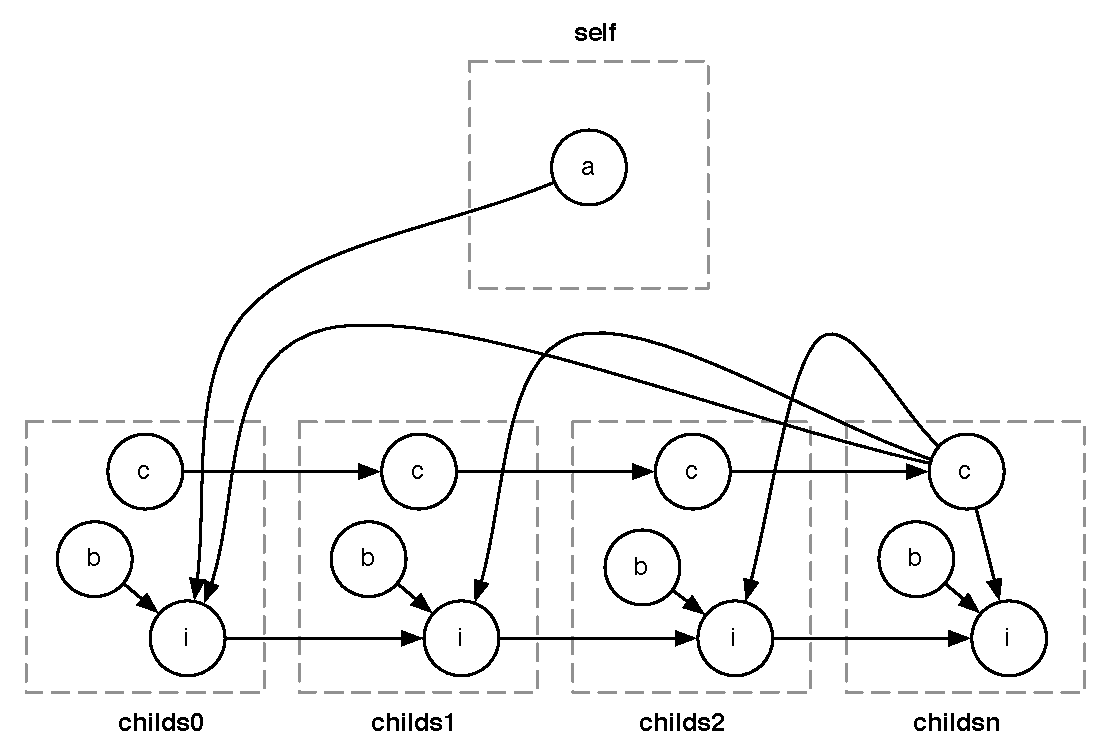
\includegraphics[trim=0 0 0 0,clip,width=0.7\columnwidth]{chapter3/unrolledloop}
\end{minipage}}\\
\subfloat[\textbf{Staging as Two Loops.}]{\label{fig:unrolling:stages}
\begin{minipage}{1\columnwidth}\centering
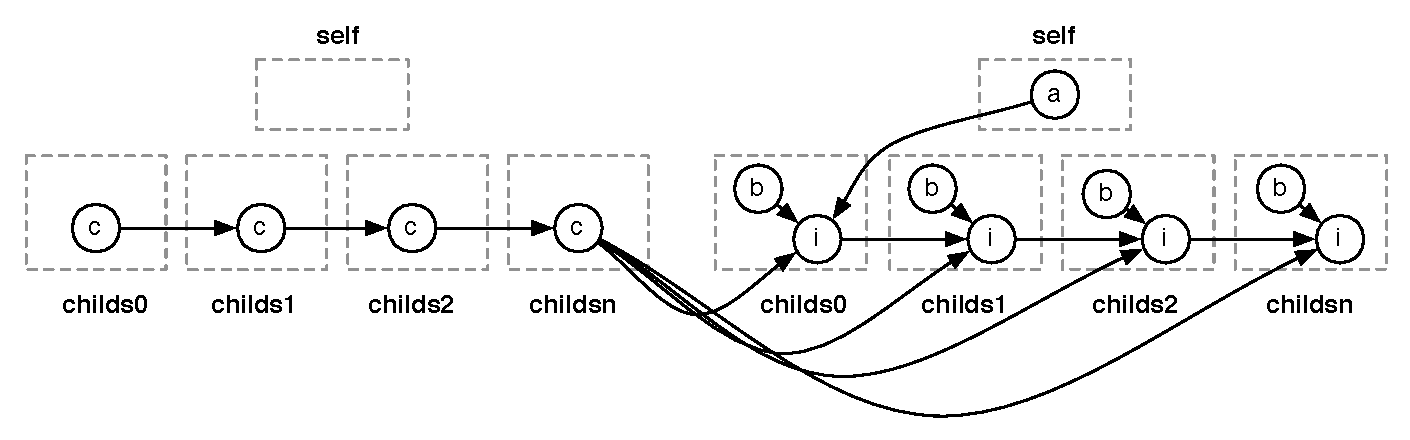
\includegraphics[trim=0 0 0 0,clip,width=1.0\columnwidth]{chapter3/stagedloop}
\end{minipage}}
\caption{\textbf{Loop scheduling}.The loop code can be scheduled as two loops that occur in the same traversal.}
\label{fig:unrolling}
\end{figure}



\subsection{Reduction to OAGs by Unrolling}
We show how to schedule the following loop:

\begin{lstlisting}[mathescape]
interface NodeI {
  var c : int;
  var i : int;
  input a : int;
  input b : int;
}
class NodeC : NodeI {
  children {  childs : [ NodeI ]; }
  actions {
    loop childs {
      childs.c := fold 0 .. childs$\$-$.c + 1;
      childs.i := 
        fold 
        a 
        ..         
        childs$\$-$.i  + childs$\$i$.b + childs$\$$.c;
    }
  }
}
\end{lstlisting}

Our reduction unrolls the loop into 4 steps ($0$, $1$, $2$, and $n$):

\begin{lstlisting}[mathescape]
interface NodeI {
  var c : int;
  var i : int;
  input a : int;
  input b : int;
}
class NodeC : NodeI {
  children {  
    childs0, childs1, childs2, childsn : NodeI;
  }
  actions {   
    childs0.c := 0 + 1;
    childs1.c := childs0.c + 1;
    childs2.c := childs1.c + 1;
    childsn.c := childs2.c + 1;

    childs0.i := a + childs0.b + childsn.c;
    childs1.i := childs0.i + childs1.b + childsn.c;
    childs2.i := childs1.i + childs2.b + childsn.c;
    childsn.i := childs2.i + childsn.b + childsn.c;
  }
}        
\end{lstlisting}



The reduction performs several rewrites that unroll loops and then substitute variable names in the unrolled statements:

\begin{figure}
\begin{align*}
\llbracket ~child : [ interface ] ~\rrbracket &\rightarrow child0, child1, child2, child \texttt{n} : interface 
\\
\llbracket child.fld := \texttt{fold} ~ e_{\texttt{init},fld} ~ .. ~ e_\texttt{step} \rrbracket &\rightarrow 
\\
& child0.fld = \llbracket~e_\texttt{step}[\forall ~f:  ~ e_{\texttt{init},f} ~/~ child\$\texttt{-}.f~]~\rrbracket_0; 
\\
& child1.fld = \llbracket~e_\texttt{step}~\rrbracket_1; 
\\
& child2.fld = \llbracket~e_\texttt{step}~\rrbracket_2; 
\\
& childn.fld = \llbracket~e_\texttt{step}~\rrbracket_\texttt{n} 
\\
\llbracket ~child\$\$.fld ~\rrbracket_\alpha &\rightarrow child \texttt{n}. fld
\\
\llbracket ~child\$i.fld \rrbracket_\alpha & \rightarrow child\alpha.fld
\\
\llbracket ~child\$\texttt{-}.fld \rrbracket_1 & \rightarrow child0.fld
\\
\llbracket ~child\$\texttt{-}.fld \rrbracket_2 & \rightarrow child1.fld
\\
\llbracket ~child\$\texttt{-}.fld \rrbracket_\texttt{n} & \rightarrow child2.fld
\end{align*}
\caption{\textbf{Rewrite Rules for Loop Reduction}. Cases of $\llbracket \cdot \rrbracket$ that simply recur are elided.}
\label{fig:loopreduction}
\end{figure}


\subsection{Recovery by Commuting Abstractions}





\section{Verification}

We automatically check an attribute grammar and its schedule for safety. This section focuses on two aspects of our approach: the properties to verify and the modular design of the verification procedure. The properties are significant in that they cover both functional and behavioral correctness, and are typically desired but not proven for layout languages and pattern programs. Furthermore, we check the properties through axiomatic reasoning parameterized by a local dependency analysis. This proof structure simplifies extending the language of statements and of schedules as most additions correspond to an isolated and com posable axiom. Later, in Chapter~\ref{chap:4}, we show a simple approach to changing the verifier into a synthesizer and thereby achieve fully automatic or computer-assisted parallelization.

Our approach automatically checks three properties. 
\begin{itemize}
\item \textbf{Totality} The specification defines one and only one solution for every well-formed input tree. 
\item \textbf{Determinism} The schedule evaluates the constraints of the attribute grammar without any data races.
\item \textbf{Linearity (Single Assignment)} Every attribute is assigned exactly once. Layout languages often perform \emph{reflow} to iteratively solve constraints or incremental computation, verifies that reflow is strictly an optimization.
\end{itemize}
In this chapter, we illustrate how to check race freedom. The check for linearity is similar , and totality is a consequence of the determinism and linearity properties.

We focus on a modular checking strategy for two reasons. First, we encountered implementation challenges without it. Our initial attempts to adapt the OAG~\cite{oag} algorithm, which is a search over a global dependency graph, suffered from many implementation bugs before we abandoned it. Our new approach instead decouples verification from synthesis and pattern checking from dependency analysis. Second, challenging our OAG implementation and the basic premise of our approach, we need to support adding new types of traversals. New schedule combinators, such as nested traversals, and individual patterns, such as recursive, should be simple to add as new types of parallel patterns are understood. Adding a parallel pattern should not require refactoring the entire verifier or synthesizer. Our new approach phrases each pattern as an independent axiom and automatically incorporates it into the checking procedure.



 \newcommand{\bigforall}[2]{{{\raisebox{-6pt}{\mbox{\Large$\forall$}$#1$}}\atop{\scriptstyle #2}}}

 


\begin{figure}[t]
\centering

$\begin{array}{c}
  $$\inference{ 
    \{ A \} ~p~ \{ B \} ~~~~~~~~ \{ B \} ~q~ \{ C \}
  }{ 
    \{ A \} ~p ~ ; ~ q~ \{ C \}
  }[  ]$$
\rrule{(seq)} \\ \vspace{1em} \\ 

$$\inference{ 
    \{ A \} ~p~ \{ B \} ~~~ \{ A \} ~q~ \{ C \}}{ 
    \{ A \} ~p ~ || ~ q~ \{ B \cup C \}
  }[ ]$$
\rrule{(par)} \\ \vspace{1em} \\

$$\inference{ 
Regions = \{\alpha \mapsto Visit*_\alpha\} ~ \cup ~ \displaystyle \bigcup_{i} \{\beta_i \mapsto Visit_i* \} \hfill \\
\forall~~ (\gamma \mapsto Visit*) \in Regions:  \hfill \\
~~~~ C_\gamma = \texttt{alwaysCommunicate}_\alpha(\gamma, B, Regions) \hfill \\
~~~~ \{ A, C_\gamma \} ~~ \gamma~Visit* ~~ \{ A \cup B_\gamma \} \hfill
}{ \{ A \} ~~ \alpha~  ~ Visit*_\alpha \{(\beta_i \mapsto Visit_i)* \}? ~~ \{ A \cup ~ \bigcup B_\gamma \} }[]$$
\rrule{(nest_\alpha)} \\ \vspace{1em} \\


$$\inference{
P = \cup Prod_i~~~~ Steps =  \cup Step_j \\
B = \displaystyle \bigcup_{i}\hfill\
\texttt{reachable}_\beta(Prod_i, P, A,Steps, C)}
{ \{ A , C \} ~~ \beta ~(Prod_i~\{~Step_j*~\})*  ~~ \{ A \cup B \}}[]$$
\rrule{(check_{\beta})} \\ \vspace{1em} %\\

%$$\inference{\{A\}~p~\{B\}~~~~ unify(sketch,p)}{\{ A \} ~ p \wedge sketch ~ \{ B \} }[]$$
%\rrule{(sketch)} 
\end{array}$  

%\begin{lstlisting}[mathescape]
%set unreachable($\beta$,$P$,$A$,$B$,$C$):
%  reachable := $\displaystyle \bigcup_{p \in P}$ reachable$_\beta$($p$, $A$, %$B$, $C$)
%  return B $-$ reachable
%\end{lstlisting}

\caption{Correctness axioms for checking a schedule}
\label{fig:deductions}
\end{figure}


\newsavebox{\parcheckers}
\begin{lrbox}{\parcheckers}% Store first listing
\begin{minipage}{1\columnwidth}
\centering
\begin{lstlisting}[mathescape,escapechar=\`,morekeywords={set,return}]
set reachable$_\texttt{parPre}$($W{\rightarrow}X$,$P$,$A$,$B$,$C$):  
  reach :=
    $~~~~ \{ a_{*,W{\rightarrow}X} ~ | ~ a_{*,W{\rightarrow}X}  \in A \} \cup~ (C \cap \{ a_{W,W{\rightarrow}X} ~ | \displaystyle \bigwedge _{V{\rightarrow}W \in P} W.a_{V{\rightarrow}W} \in B \}) \cup ~(C \cap \{ a_{X,W{\rightarrow}X}  ~ |  \neg \exists X{\rightarrow}Y \in P\})$
  while true:    
    progress := $\{ a_{*,W{\rightarrow}X} ~|~  a_{*,W{\rightarrow}X} = f(b_0, \ldots, b_n) \in \texttt{F}$ `\Suppressnumber` $\displaystyle \wedge ~ a_{*,W{\rightarrow}X} \in B ~ \wedge ~~ \bigwedge b_i \in ~$reach$\}$ `\Reactivatenumber`
    reach := reach $\cup$ progress
    if progress = $\emptyset$:
      break
  return reach  
\end{lstlisting}
\end{minipage}
\end{lrbox}

\newsavebox{\comcheckers}
\begin{lrbox}{\comcheckers}
\begin{minipage}{1\columnwidth}
\centering
\begin{lstlisting}[mathescape,escapechar=\`,morekeywords={set,return}]
$\texttt{alwaysCommunicate}_\texttt{parPre}(\beta, B, M) = \hfill$
  $\{ a_{W,W{\rightarrow}X} ~ | ~ (W{\rightarrow}X~B_\beta) \in M[\beta] ~~  \displaystyle \bigwedge _{(V{\rightarrow}W~B_\gamma) \in M[\gamma \neq \beta]}  a_{W,V{\rightarrow}W} \in B \cup A \} $
\end{lstlisting}

%\begin{lstlisting}[mathescape,escapechar=\`,morekeywords={set,return}]
%$\texttt{alwaysCommunicate}_\texttt{parPost}(\beta, B, M) = \hfill$
%  $\{ a_{X,W{\rightarrow}X} ~ | ~ (W{\rightarrow}X~B_\beta) \in M[\beta] $
%           $~ \wedge ~ \displaystyle \bigwedge _{(X{\rightarrow}Y~B_\gamma) \in M[\gamma %\neq \beta]}  a_{X,X{\rightarrow}Y} \in B \cup A \} $
%\end{lstlisting}


%\begin{lstlisting}[mathescape,escapechar=\`,morekeywords={set,return}]
%$\texttt{alwaysCommunicate}_\texttt{recursive} = %\texttt{alwaysCommunicate}_\texttt{parPre}$
%\end{lstlisting}

\end{minipage}
\end{lrbox}


\begin{figure}[t]
\subfloat[Communication check for region boundaries in a \sched{parPre} traversal]{
\label{fig:comm}
\usebox{\comcheckers}
} \\
\subfloat[ Unoptimized production visit check for \sched{parPre} traversal]{
\label{fig:parprecheck}
\usebox{\parcheckers}
}
\caption{Inter- and intra-region checkers for \sched{parPre}.}
\label{fig:checkers}
\end{figure}
 
 

\subsection{Axiomatic Correctness Checking}

%%%%%%

Correctness axioms for checking an entire schedule are in Figure~\ref{fig:deductions}. The judgements recursively check a composition of traversals until reaching the traversal-specific checks of Figure~\ref{fig:checkers}. Checking tames worst-case time linear in the number of attributes and the number of their local dependencies. As a reminder, Figure~\ref{fig:hboxparallel:decomplang} defines the language of schedules.

We use a small amount of notation. Variables $p$ and $q$ denote schedules (\lstinline{<Sched>}), $A$ and $B$ are sets of attributes, and $\alpha$ and $\beta$ are traversal types (\lstinline{<travAtomic>}). Attribute $a_{W, V{\rightarrow}W}$ is decorated with its production ($V{\rightarrow}W$) and the non-terminal within it ($W$). We write  $a_{*, V{\rightarrow}W}$ if $a$ can be associated with a non-terminal on either side of the production.

The rules to check composition and individual traversals are as follows:

\paragraph*{Sequential and parallel composition: ``\sched{;}'' and ``\sched{||}''}The simplest composition check is for sequencing: Hoare triple ``\sched{\{A\} p ; q \{C\}}'' (rule $\rrule{{seq}}$).  If attributes $A$ are solved before traversal ``\sched{p ; q}'', then attributes $C$ will be solved after. The conditions above the judgement bar state this is true if $p$ can always compute attributes $B$ given attributes $A$, and $q$ can always then compute $C$. The judgement is recursive. Analogous reasoning explains  ``\sched{||}'' (rule $\rrule{{par}}$).

%\paragraph*{}
%We split checking one traversal over the tree into two rules:

\paragraph*{Nested composition: $\mapsto$}
Rule $\rrule{{nest}_\alpha}$ checks outer traversal type $\alpha$ over regions where each one may have its own traversal type $\gamma$. Consider an outer traversal type of  \sched{parPre}: as it progresses top-down, every region might be guaranteed to have attributes of its root node solved before evaluation proceeds within it. For each region (the set of productions mapped to region traversal type $\gamma$), the rule calls $\texttt{alwaysCommunicate}_{\texttt{parPre}}$ to find the set $C_\gamma$ of  attributes that are externally set before the region is traversed. Rule $\rrule{{nest}_\alpha}$ calls checks for every region under the assumption that $C_\gamma$ is already solved.

The first line of rule $\rrule{{nest}_\alpha}$ means that, for any outer traversal $\alpha$, attributes scheduled for the outer region are  treated as if they were in their own region ($\gamma = \alpha$). Traversals that do not use nesting are degenerate:  all the productions belong to one region ($\gamma = \alpha$).

\paragraph*{Traversal over a region (e.g., parPre)}
The schedule for a traversal of type $\beta$ over a region is correct if every production visit schedule is correct (rule $\rrule{{check}_\beta}$). A production visit schedule $Prod_i~\{~Step_j*~\}$ is correct when there is an order for computing its scheduled attributes $Step_j*$ along which all of the data dependencies of the corresponding semantic functions are satisfied. %The order exists if the transitive closure of attributes with satisfiable dependencies covers $B$. 

Traversals that do not perform nesting, such as a single occurrence of \sched{parPre}, are handled as degenerate nested composition with one region: the entire tree.

\paragraph*{Production visit}

A fast and simple checking algorithm would be to mark each attribute  of a production as dirty or clean inside a structure that persists across checks of different visits to the same production. For each successive attribute in a visit's sequence, if all of its dependencies are met (dirty), mark the attribute, and otherwise fail the check. Non-local dependencies can be handled as below.


To optimize the synthesis algorithm of Chapter~\ref{chap:4}, we use a slightly indirect algorithm to check the correctness of visiting a production.  The intuition is that it relaxes the specification of visit's attributes by treating the ordered sequence as an unordered set and checks the reachability of the set's dependency graph. 

Figure~\frefb{fig:checkers}{fig:parprecheck} shows an unoptimized reachability computation for visiting a production inside a \sched{parPre} region. It is the standard transitive closure, except for two subtleties:

First, only attributes that are meant to be scheduled are considered reachable ($B$ membership check in line 7). Incorrectly including unscheduled attributes would erroneously allow attributes with unresolved dependencies to also be included.  

Second, attributes computed by visits to adjacent productions must be distinguished. Adjacent productions may be in the same region or in another. In a \sched{parPre} region, consider when $W$ is always an intermediate node of the region and attribute $a_{W,W{\rightarrow}X} \in B$ is always set by a parent production $V{\rightarrow}W$ in the same region. For this intra-region case, $a_{W,W{\rightarrow}X}$ is guaranteed to be reachable at the beginning of the visit to $W{\rightarrow}X$.  However, if $W$ can be the root node of the region, we must also check $a_{W,V{\rightarrow}W}$ is set by adjacent regions before the root is visited. %The checks for the intra-region case and the \texttt{alwaysCommunicate} inter-region case are in lines 4-5 of $\rrule{{nest}_\alpha}$.

%\paragraph*{Sketches}
%Rule $\rrule{{sketch}}$ separates checking the correctness of a schedule from whether a sketch matches it. First, a schedule must be correct irrespective of the accompanying sketch. Second, the schedule must syntactically match the schedule ($unify$). Later, we provide semantically constrained sketches that are checked by Prolog's more general unifier (Section~\ref{sec:prolog}). 

Checking an explicit sequence reduces to checking that the transitive closure can be performed in the specified order rather then the declarative definition in Figure~\ref{fig:checkers} . The synthesizer of Chapter~\ref{chap:4} does not need to check for ordering, so we omit this check.


%%%%%%
\subsection{Property Proofs}
The axioms check for determinism, which can be adapted to check the two other properties.

First, the axioms check determinism, which means that rerunning the schedule will yield the same result.  We can check determinism by ensuring that a schedule computes the attributes of an attribute grammar without races. More precisely, it tracks what attributes are guaranteed to have been computed by any particular point of the schedule, and uses that to check that every step of the computation only relies on what is guaranteed to have been computed.

Linearity requires that that every instance of an attribute is only assigned to once. We can check linearity by extending the axioms in two ways. First, they must check that for any given attribute $X_a$, it is either defined by all productions $X \rightarrow W$ or by all productions $W \rightarrow X$. Second, for every attribute assigned in production $X \rightarrow W$, it must only be scheduled for one visit. 

Totality guarantees that every well-formed input tree yields one and only one result. It is a property of the language because any schedule must reach the same result. In contrast, determinism is a property of a schedule because, for the same language, rerunning one schedule may always return the same result while the same might not be guaranteed for another schedule. The proof of totality lies in the proof of linearity. Given a linear schedule, the dynamic dependency graph of every input document is directed and acyclic. The DAG property guarantees that the value of each node is a pure function of the values of the dominating nodes, and therefore the language has a (total) functional interpretation. Checking totality adds an additional step beyond checking linearity: totality requires that every attribute in the grammar appears in the schedule.

\subsection{Verification is $O(|A|)$}
Verifying a schedule for race-freedom takes time linear in the number of attributes. Our  description of the checker in Figures~\ref{fig:deductions} and~\ref{fig:checkers} does not show the optimizations that lead to this bound so we highlight the key ideas here.

First, the number of axioms to check is linear in the number of attributes. Every traversal computes at least one attribute, which implies that the number of traversals is bounded by the number of attributes. Only non-empty visits must be checked, and their number is likewise bounded by the number of attributes.

Second, the time to check an axiom is linearly bounded by the number of attributes (and their dependencies) to be scheduled by that axiom. For example, checking the visit to a production is effectively a topological sort of the local dependency graph restricted to the attributes evaluated during the visit. Topologically sorting dependency graph $G = (E, V)$ is $O(|E| + |V|)$. An attribute can have at most $|A|$ local dependencies so verification takes time $O(|A|)$.  For simplicity, our implementation does not use the topological sort optimization, and we only encountered performance issues on one case study due to that.

Similar reasoning applies to quickly checking the two other properties. Linear checking of linearity follows the same proof structure. Each attribute is labeled based on the type of production that solves it and rule $\rrule{{check}_\beta}$ checks that the labels of attributes in $Step_j$ match production $Prod_i$. The time to check the axiom is therefore still bounded by the number of scheduled attributes. Finally, totality checks that the computed set of attributes matches the total set, and comparing two sets is also linear in the number of attributes.







\section{Evaluation: Layout as Structured Parallel Visits}
\subsection{Box model}
\subsection{Nested text}
\subsection{Grids}


\subsection{SIMD Rendering through Staged Memory Allocation}
We evaluate three dimensions of our staged memory allocation approach: flexibility, productivity, and performance. First, it needs to be able to express the rendering tasks that we encounter in GPU data visualization. Second, it should some form of productivity benefit for these tasks. Finally, the performance on those tasks must be fast  enough to support real-time animations and interactions of big data sets.



\subsubsection{Productivity}
Productivity is difficult to measure. Before using the automation extensions for rendering, we repeatedly encountered bugs in manipulating the allocation calls and memory buffers. The bugs related both to incorrect scheduling and to incorrect pointer arithmetic. Our new design eliminates the possibility of both bugs.

One suggestive productivity measure is of how many lines of code the macro abstraction eliminates from our visualizations. We measured the impact on using it for 3 of our visualizations. The first visualization is our HBox language extended with rendering calls, while the other two are interactive reimplementations of popular visualizations: a treemap~[[CITE]] and multiple 3D line graphs~[[CITE]].


\begin{table}[ht]
\caption{Lines of Code Before/After Invoking the '@' Macro}
\centering
\begin{tabular}{c r r r}
\hline\hline
 \textbf{Visualization} & \textbf{Before (loc)} & \textbf{After (loc)} & \textbf{Decrease} \\ [0.5ex] \hline
  HBox & 97 & 54 & 44\% \\
  Treemap & 296 & 241 & 19\% \\
  GE & 337 & 269 & 20\% \\ [1ex] 
\hline
\end{tabular}
\label{table:macroreduction}
\end{table}
Table~\ref{table:macroreduction} compares the lines of code in visualizations before and after we added the macros. Using the macros eliminated 19--44\% of the code. Note that we are \emph{not} measuring the macro-expanded code, but code that a human wrote.



As shown in Figure~\ref{fig:stagedallocClient}, the eliminated code is code that was introduced by staging the library calls. Porting unstaged functional graphics calls to the library, is in practice, an alpha renaming of function names.  Using the '@' macro eliminates 19--44\% of the code that would have otherwise been introduced and completely eliminates two classes of bugs (scheduling and pointer arithmetic), so the productivity benefit is non-trivial. 

\subsubsection{Performance}


\section{Related Work}
Lang of schedules
\begin{itemize}
\item background
\item stencils and skeletons: wavefront, ...
\item polyhedra
\end{itemize}
Schedule verification
\begin{itemize}
\item compare to OAG etc., looser dataflow/functional langs
\end{itemize} %schedule sketching

\chapter{Interacting with Automatic Parallelizers through Schedule Sketching}

\section{Automatic Parallelization: The Good, the Bad, and the Ugly}

\subsection{The Good: Automating Dependency Management}
\subsection{The Bad: Guiding Parallelization}
\subsection{The Ugly: Preventing Serialization}

\section{Holes}
\section{Generalizing Holes to Unification}

\section{Case Studies: Sketching in Action}
Show use in CSS and data viz: 
\begin{itemize}
\item when automatic is fine
\item when sketch needed for checking/debugging
\item when sketch needed for sharing
\end{itemize}

\section{Related Work}
\begin{itemize}
\item sketch, sketch for concurrent structures
\item oopsla paper for individual traversals
\end{itemize}
 %schedule synthesis
\chapter{Parallel Schedule Synthesis}
\label{chap:4}


Programmers struggle to map applications into parallel algorithms. Going beyond the automatic schedule verification of the last chapter, we now examine how to automatically generate a schedule.  Consider two of the decisions that a programmer faces in manually designing a schedule:
\begin{itemize}
\item \textbf{Scheduling a single traversal.} Many computations contain sequential dependencies between nodes. One correct traversal over the full tree might then be sequential. However, if the sequential dependencies can be isolated to a subtree, an overall parallel traversal would be possible if it invokes a sequential traversal for just the isolated subtree. Whether such isolation is always possible is not obvious.
\item \textbf{Scheduling multiple traversals.} Programs such as browsers perform many traversals. Traversals might run one after another, concurrently, or be fused into one. These choices optimize for different aspects of the computation. Running two traversals in parallel improves scaling, but fusing them into one parallel traversal avoids overheads: the choice may depend on both the hardware and tree size. Which traversal sequence to use is not obvious.
\end{itemize}
These decisions explode the space of schedules. Today, programmers manually navigate the space by selecting a parallel schedule, judging its correctness,  and comparing its efficiency to alternative schedules. The tasks are expensive: programmers  globally reason about dependencies, develop prototypes for profiling, and whenever the functional specification changes, restart the process. 

This chapter explores the design and implementation of an attribute grammar that supports automatic schedule synthesis.
We examine several questions: 
\begin{itemize}
\item What programming constructs are enabled by schedule synthesis?
\item What is an algorithm to \emph{quickly} find a \emph{correct} schedule?
\item If multiple schedules are possible, how do we find a \emph{fast} one?
\end{itemize}
The following sections explore each question in turn. 



\section{Computer-Aided Programming with Schedule Holes}
\label{sec:holes}
Being able to automatically generate parallel schedules enables rich forms of parallel programming. An automation tool will automatically find a parallel schedule, so a natural conclusion would be to assume the programming interface would hide all parallelization concerns. We found this to be largely true when writing small amounts of declarative data visualization code. However, in parallelizing the larger and more complicated CSS layout language, we encountered cases where the visualization designer needed to guide (or be guided by) the automation procedure. Likewise, we encountered the need for one programmer to communicate parallel structure to another. Automatic parallelization is insufficient in that hides all parallelization details, yet manual scheduling was too low-level and brittle.

Our solution is to provide a \emph{sketching} construct for specifying constraints on the schedule that the automatic parallelization algorithm must respect. We routinely wrote schedules sketches in order to override schedule selection, test and debug parallelization ideas, and enforceably communicate parallelization decisions when sharing code with others. Discussed later in this chapter~\ref{??}, we also used the sketching mechanism to speed up automatic parallelization over specifications with many attributes or schedule patterns that challenge static analysis.

We revisit the specification of \hlang{} to demonstrate the sketching construct and its use for the above scenarios. First, many parallel schedules are possible for \hlang{}, and if we  have a preference, ...

\begin{align}
%\begin{lstlisting}[mathescape,morekeywords={parPre,parPost}]
\text{\textbf{parPost}} ~ \hole_1 ~ ; ~ \text{\textbf{parPre}} ~ \hole_2 \\
(\text{\textbf{parPost}} ~ \hole_3 ~ ; ~ \text{\textbf{parPost}} ~ \hole_4) ~ ; ~ \hole_5 \\
\hole_6
\end{align}






\subsection{Generalizing Holes to Unification}

\section{Fast Schedule Synthesis}
\subsection{Search}
\subsection{Optimization}
\subsection{Analysis}

\section{Schedule Autotuning}
\label{sec:schedtuning}
\subsection{Alternation Heuristic: Off-by-one Optimality}
\subsection{Enumeration via Incrementalization}

\section{Evaluation}
\subsection{Case Studies: Sketching in Action}
Show use in CSS and data viz: 
\begin{itemize}
\item when automatic is fine
\item when sketch needed for checking/debugging
\item when sketch needed for sharing
\end{itemize}
\subsection{Speed of synthesis}
Success, fail, enumerate
\subsection{Line counts of extensions}
\subsection{Loss from greedy heuristic}
\subsection{Benefit from autotuning}


%
%
%\chapter{Interacting with Automatic Parallelizers through Schedule Sketching}
%
%\section{Automatic Parallelization: The Good, the Bad, and the Ugly}
%
%\subsection{The Good: Automating Dependency Management}
%\subsection{The Bad: Guiding Parallelization}
%\subsection{The Ugly: Preventing Serialization}
%
%\section{Holes}
%\section{Generalizing Holes to Unification}
%
%\section{Case Studies: Sketching in Action}
%Show use in CSS and data viz: 
%\begin{itemize}
%\item when automatic is fine
%\item when sketch needed for checking/debugging
%\item when sketch needed for sharing
%\end{itemize}
%
%\section{Related Work}
%\begin{itemize}
%\item sketch, sketch for concurrent structures
%\item oopsla paper for individual traversals
%\end{itemize}
 %MIMD, SIMD, SIMT
\chapter{Optimizing Tree Traversals for MIMD and SIMD}
\label{chap:6}
\section{Overview}

For a full language, statically identified parallelization opportunities still require an efficient runtime implementation that exploits them. In this section, we show how to exploit the logical concurrency identified within a tree traversal to optimize for the architectural properties of two types of hardware platforms: MIMD (e.g., multicore) and SIMD (e.g., sub-word SIMD and GPU) hardware. For both types of platforms, we optimize the schedule within a traversal and the data representation. We innovate upon known techniques in two ways:

\begin{enumerate}
\item \textbf{Semi-static work stealing for MIMD:} MIMD traversals should be optimized for low overheads, load balancing, and locality. Existing techniques such as work stealing provide spatial locality and, with tiling, low overheads. However, dynamic load balancing within a traversal leads to poor temporal locality across traversals. The processor a node is assigned to in one traversal may not be the same one in a subsequent traversal, and as the number of processors increases, the probability of assigning to a different one increases. Our solution dynamically load balances one traversal and, due to similarities across traversals, successfully reuses it.
\item \textbf{Clustering traversals for SIMD:}  SIMD evaluation is sensitive to divergence across parallel tasks in instruction selection. Visits to different types of tree nodes yield different instruction streams, so na\i{v}e vectorization fails for webpages due to their visual variety. Our insight is that similar nodes can be semi-statically identified. Thus \emph{clustered} nodes will be grouped in the data representation and run in SIMD at runtime.
%\item \textbf{Automatically staged parallel memory allocation to efficiently combine SIMD layout and SIMD rendering:} We optimized the schedule of memory allocations in the layout computation into an efficient parallel prefix sum. Otherwise, parallel dynamic memory allocation requests would contend over the free memory buffer and void GPU performance benefits. We automated the optimization by reducing the scheduling problem to attribute grammar scheduling and automatically performing the reduction through macro expansion.
\end{enumerate}

Our techniques are important and general. They overcame bottlenecks preventing seeing any speedup from parallel evaluation for webpage layout and data visualization. Notably, they are generic to computations over trees, not just layout. An important question going forward is how to combine them as, in principle, they are complementary.

\section{MIMD: Semi-static work stealing}
We optimize the tree data representation and runtime schedule for MIMD evaluation. We did not see significant parallel speedups when either one was left out. Through a non-trivial amount of experimentation, we found an almost satisfactory combination of existing techniques. It includes popular ideas such as work stealing~[[CITE]] for load-balanced runtime scheduling and tiling~[[CITE]] for data locality, so we report on how to combine them. However, we did not see more than 2X speedups until we added a novel technique to optimize for low  run-time scheduling overheads and temporal data locality: semi-static work stealing. The remainder of this section explores our basic data representation and runtime scheduling techniques.


\begin{figure}
\centering
\subfloat[Na\"{i}ve pointer-based tree representation]{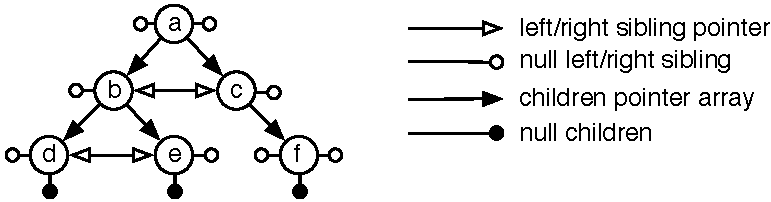
\includegraphics[width=0.6\columnwidth]{chapter6/treenaive}\label{subfig:pointer}} \linebreak
\subfloat[Compressed tree encoding]{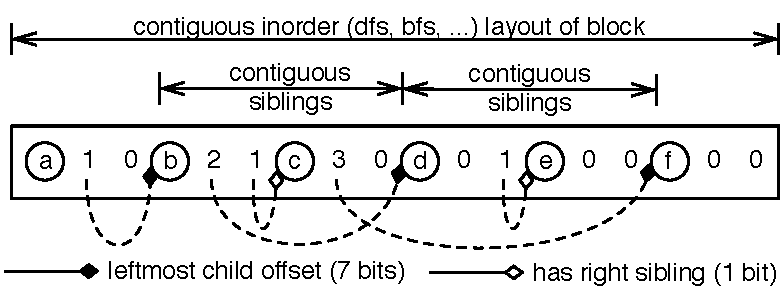
\includegraphics[width=0.6\columnwidth]{chapter6/treecompressed}\label{subfig:compressed}}
\caption{Two representations of the same tree: na\i{v}e pointer-based and optimized. The optimized version employs packing, breadth-first layout, and pointer compression via relative indexing.}
\label{fig:compression}
\end{figure}


\subsection{Data representation: Tuned and Compressed Tiles}

Our data representation optimizes for spatial and temporal locality and, as will be used by the scheduler, low overheads for operating over multiple nodes. Many researchers have proposed individual techniques for similar needs, and it is unclear which to use for what hardware. For example, mobile devices typically have smaller caches than laptops, they should exchange time for space. Our solution was to implement many techniques and build an autotuner~[[CITE]] that automatically choose an effective combination.  

Our autotuner runs sample data on multiple configurations for a particular platform to decide which configuration to use. The most prominent options are:

\begin{itemize}
\item C++ collections or contiguous arrays
\item tiling~\cite{tiling} of subtrees
\item depth-first or breadth-first ordering of nodes in a tile (with matching traversal order~\cite{Chilimbi:1999})
\item aligned data, or unaligned but more packed data
\item pointer compression
\end{itemize}
Several of the techniques are parameterized, so our tuner performs a brute force search for parameter values such as the maximum size of a subtree tile. To make the search tractable, we prune by manually providing heuristics, such as for parameter ranges.

The individual optimizations target several objectives:

\begin{itemize}
\item \textbf{Compression} Compressing the tree better utilizes memory bandwidth and decreases the working set size. We use two basic techniques: structure packing and pointer compression. Packing combines several fields in the same word of memory, such as storing 32 boolean attributes in one 32bit integer field. Similar to \citeauthor{compression}~\cite{compression}, compression encodes node references as relative offsets (16--20bits) rather than 32bit of 64bit pointers. Likewise,  as there are typically few siblings, instead of a counter of number of children (or siblings), we use an \code{isLastSibling} bit. Figure~\ref{fig:compression} depicts a tree using pointers and one of our representations: in the example, the compressed form uses 96\% fewer bits on a 64-bit architecture.

\item \textbf{Temporal and Spatial Locality}  The above compression optimizations improve locality by decreasing the distance between data. To further improve locality, we support rearranging the data in several ways .

Tiling~\cite{tiling} cuts the tree into subtrees and collocates nodes of the same subtree. It improves spatial locality because a node only reads and writes to its neighbors. Likewise, we support breadth-first and depth-first node orderings within a subtree (and across subtrees). Such a representation matches the tree traversal order~\cite{Chilimbi:19999} and therefore improves temporal locality. 

\item \textbf{Prefetching} We supports several options for prefetching to avoid waiting on data reads.  First,  the data access patterns with the data layout, so hardware prefetchers might automatically predict and prefetch data. Second, our compiler can automatically insert explicit prefetch instructions as part of the traversal. Finally, runahead processing~\cite{runaheadprocessing} pre-executes data access instructions. A helper thread traverses a subtree ahead of a corresponding evaluator thread, requesting node data while the evaluator is still computing an earlier thread. We only saw benefits of the first in practice, but leave the others as tunable.


\item \textbf{Parallel scheduling.} Reasoning about individual nodes, such as for load balancing and synchronization, leads to high overheads. By scheduling tiles rather than nodes, we cut overheads. Nodes correspond to tasks in our system, so our approach is a form of \emph{coarsening}. Furthermore, different synchronization strategies are possible for tiles, such as whether to use spin locks, so we autotune over the implementation options. 

We also support several scheduling options. First, we support third-party task schedulers, including Intel TBB~[[CITE]], Cilk~[[CITE]], and those of TesselationOS~[[CITE]]. Second, we built our own that uses a variant of work-stealing threads pinned to processors. It includes options such as whether to use hyper threads or not, and as we saw low speedups when using multiple sockets, how many threads to  use. Our autotuner picks between scheduler implementations.

\end{itemize}

Figure~\ref{fig:compression} depicts several of the data representation optimizations: packing, pointer compression, and a breadth-first layout. 




\begin{figure}
\centering
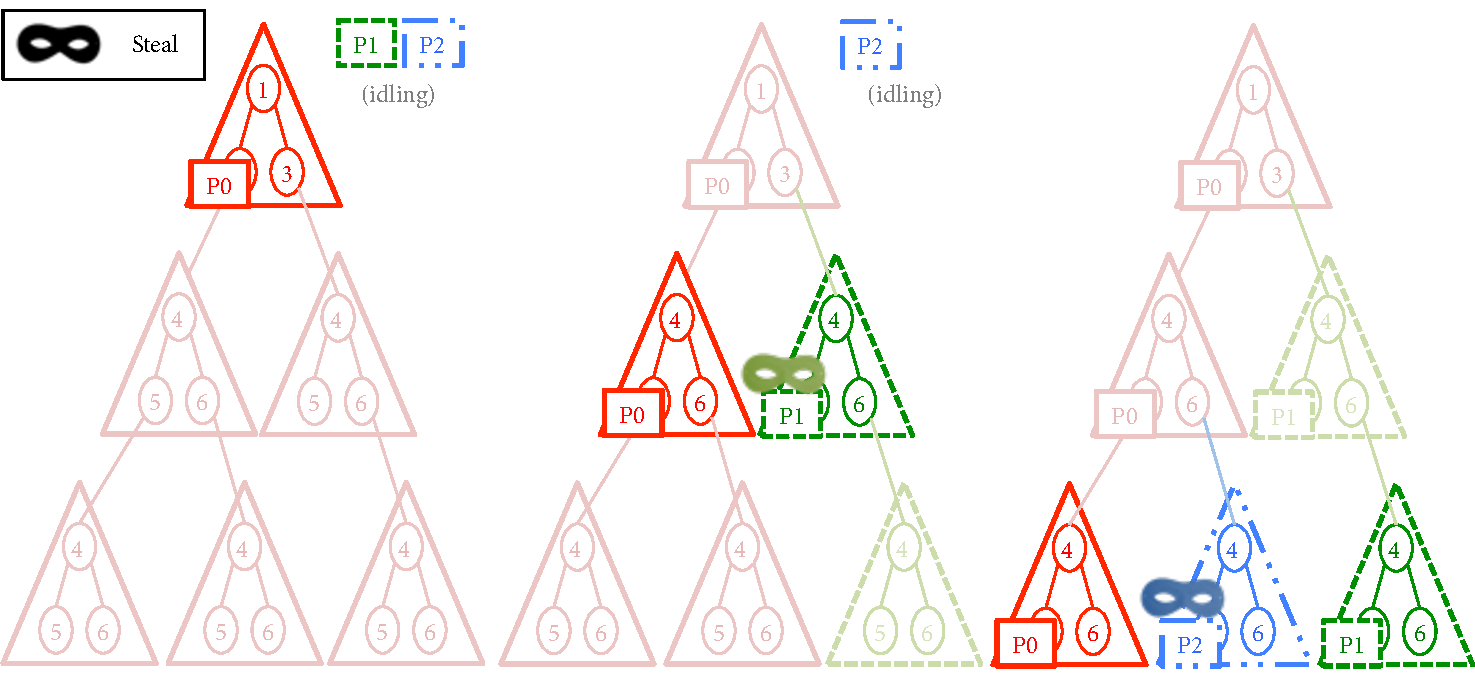
\includegraphics[width=1.0\columnwidth]{chapter6/wssimulation}
\caption{\textbf{Simulation of work stealing.} Top-down simulated tree traversal of a tiled tree by three processors in three steps.}
\label{fig:wssimulation}
\end{figure}


\begin{figure}
\centering
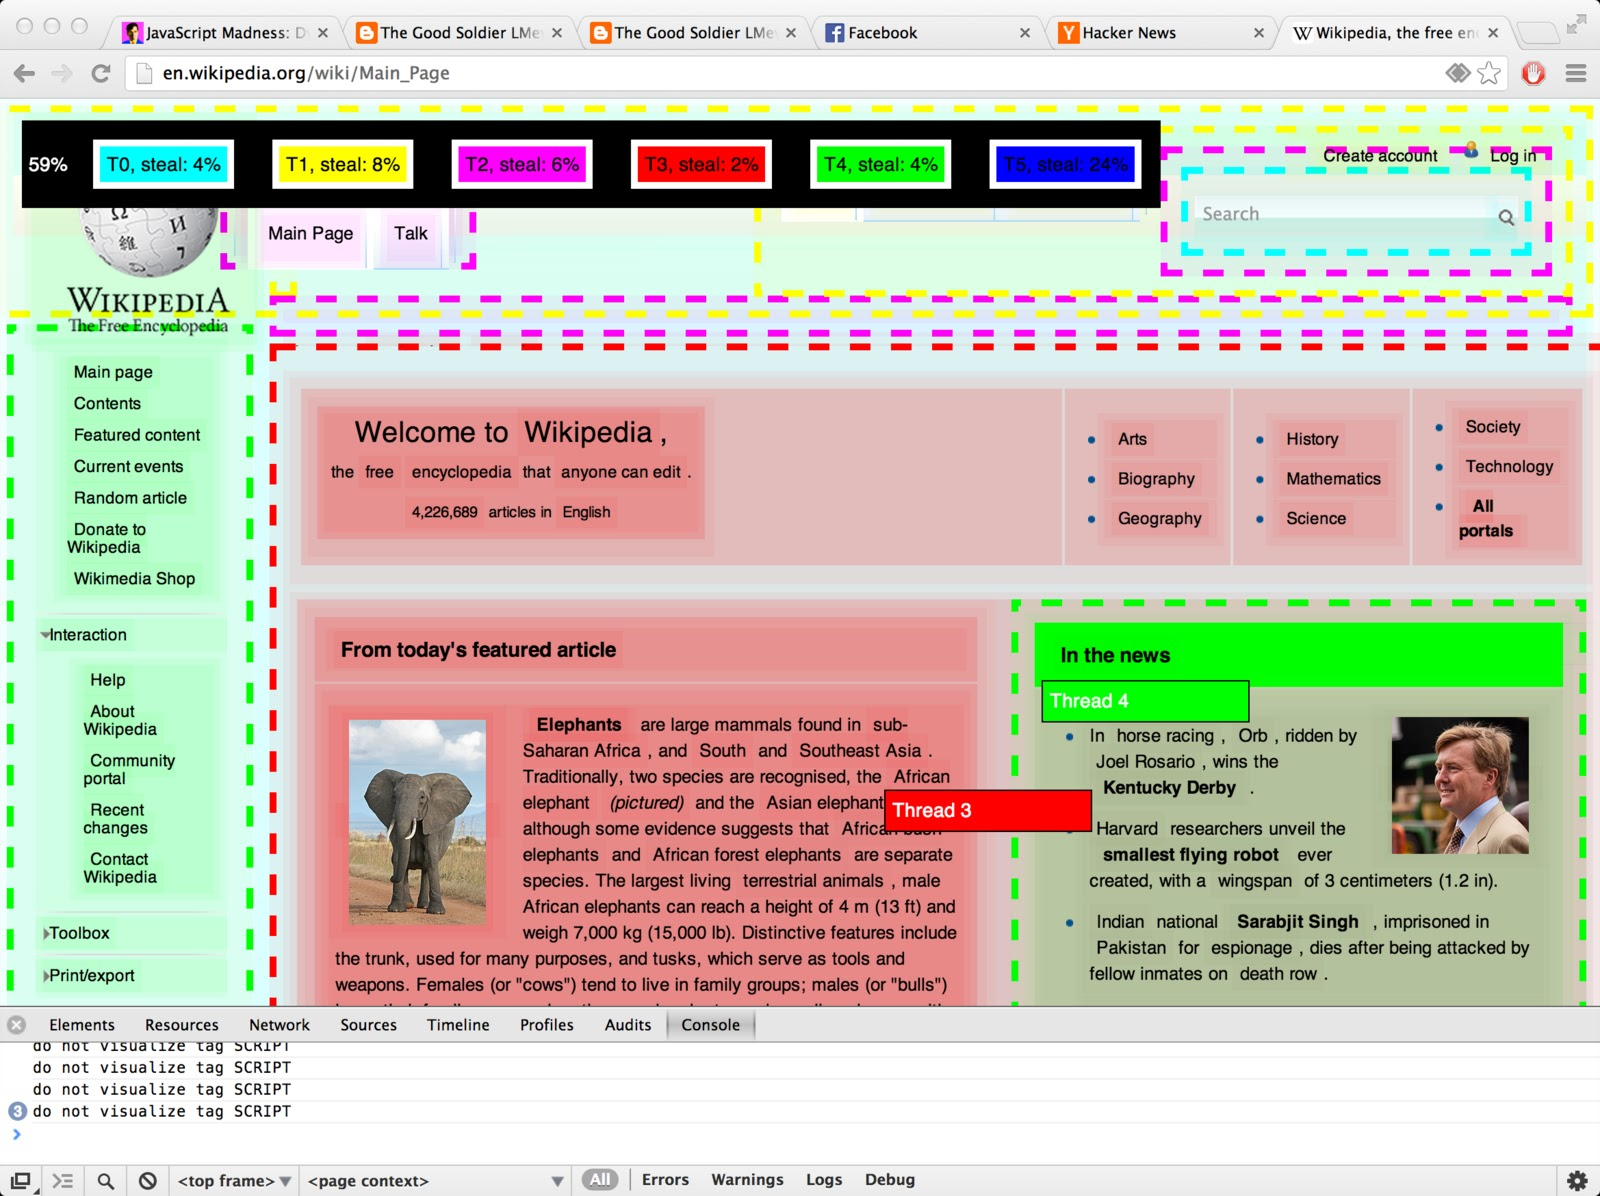
\includegraphics[width=1.0\columnwidth]{chapter6/workstealviz}
\caption{\textbf{Simulation of work stealing on Wikipedia.} Colors depict claiming processor and dotted boundaries indict subtree steals. Top-left boxes measure hit rate for individual processor.}
\label{fig:wswikipedia}
\end{figure}



\begin{figure}
\centering
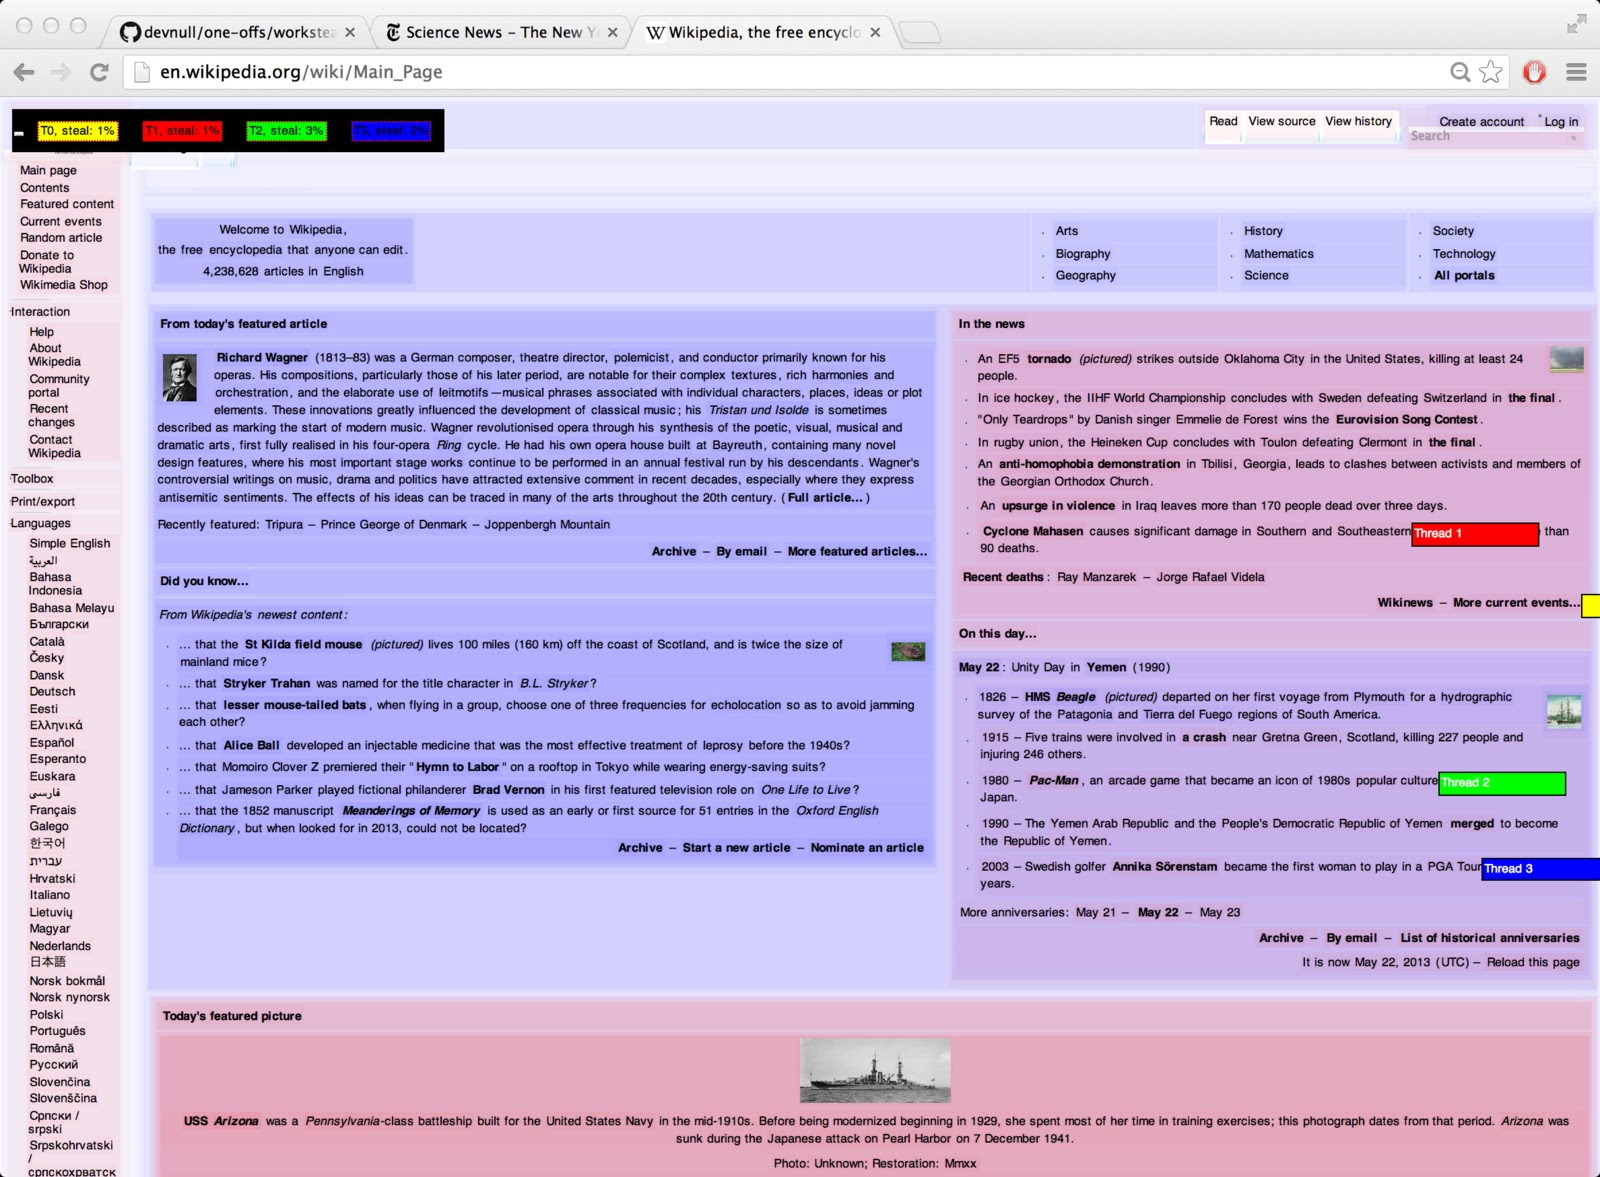
\includegraphics[width=1.0\columnwidth]{chapter6/workstealdelta}
\caption{\textbf{Temporal cache misses for simulated work stealing over multiple traversals.} Simulation of 4 threads on Wikipedia. Blue shade represents a hit and red a miss. 67\% of the nodes were misses. Top-left boxes measure hit rate for individual processor.}
\label{fig:wswikipediadelta}
\end{figure}

\begin{figure}
\centering
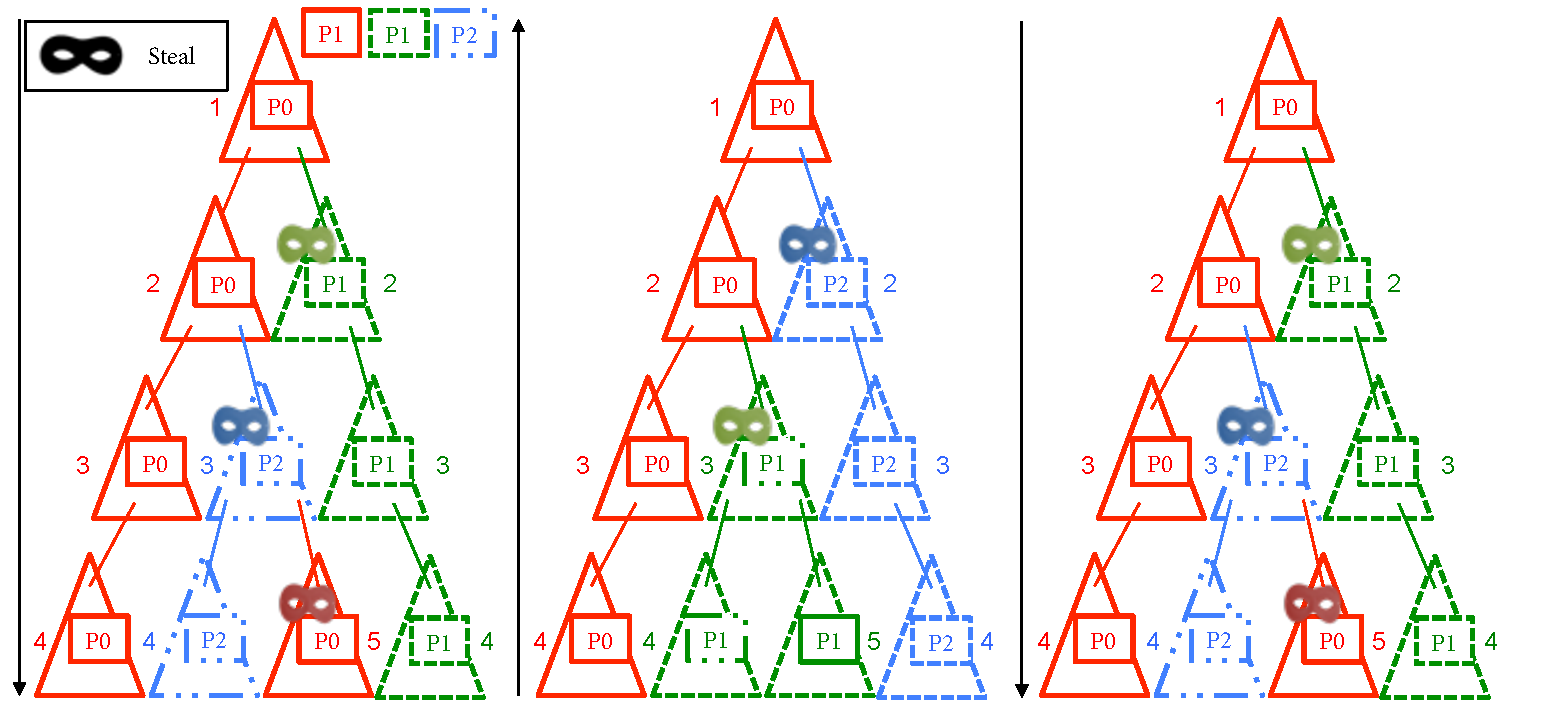
\includegraphics[width=1.0\columnwidth]{chapter6/wsbad}
\caption{\textbf{Dynamic work stealing for three traversals.} Tiles are claimed by different processors in different traversals.}
\label{fig:wsbad}
\end{figure}

\begin{figure}
\centering
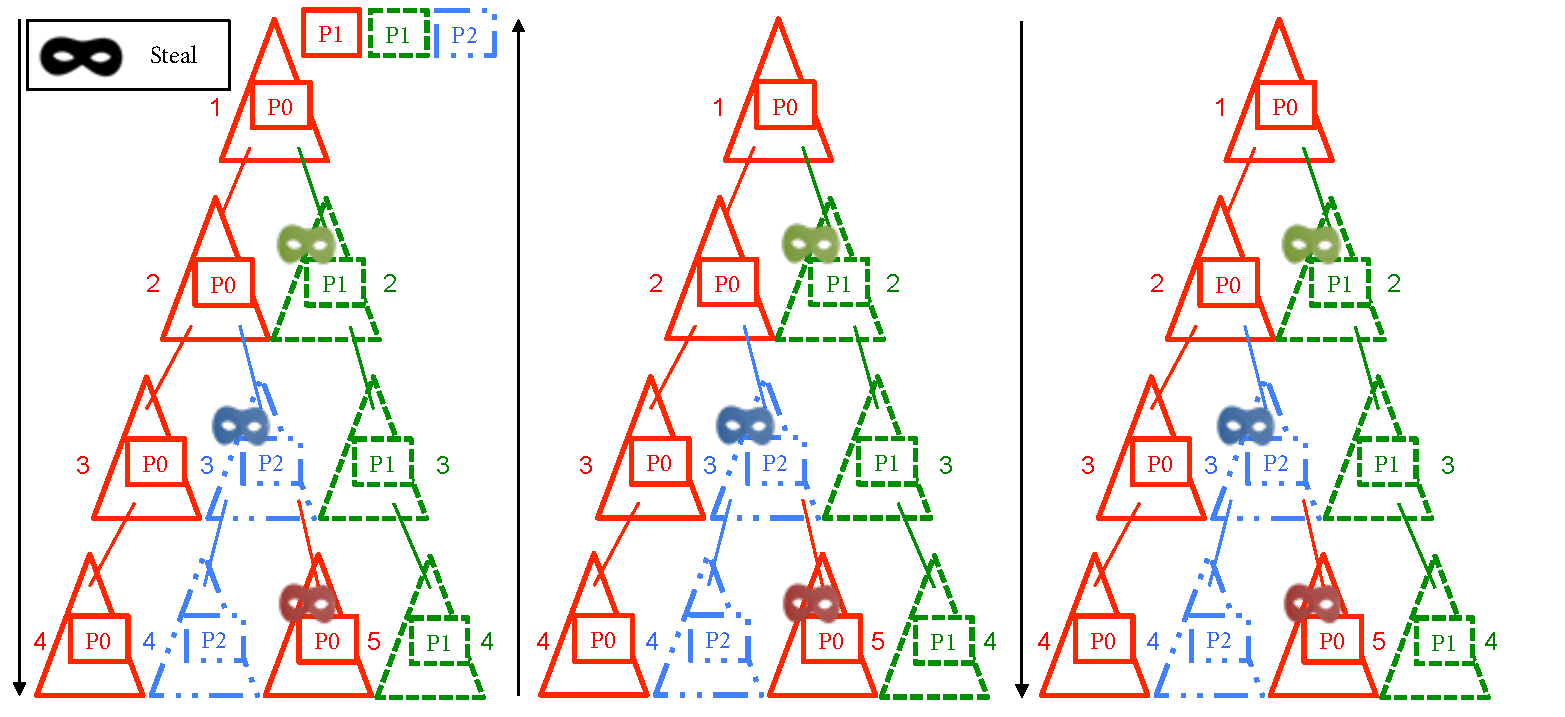
\includegraphics[width=1.0\columnwidth]{chapter6/wsgood}
\caption{\textbf{Semi-static work stealing.} Dynamic schedule for first traversal is reused for subsequent ones.}
\label{fig:wsgood}
\end{figure}


\subsection{Scheduling: Semi-static Work Stealing}
We optimize our tree traversal task scheduler for low overheads, high temporal and spatial data locality, and load balancing. Webpages are relatively small and use many traversals, so we found that aggressively optimizing individual traversals to be an important implementation concern. Our approach is to combine static scheduling~[[CITE]] with dynamic work stealing. We semi-statically schedule a traversal over the tree to as soon as it is available and reuse that schedule across traversals: this optimizes for temporal locality and low over-heads. We use work stealing as a heuristic for computing the first tree traversal for approximate load balancing.  We did not see significant speedups with the base approaches on their own, but our combination led to 7X parallel speedups. 


Our algorithm schedules the first traversal using work stealing~[[CITE]]. Work stealing was introduced as a dynamic scheduling algorithm that provides load balancing and spatial locality. Figure~\ref{fig:wssimulation} depicts a trace of three processors performing work stealing. Each processor operates on an internal task queue, and whenever a processor exhausts its internal queue, it will \emph{steal} from another processor's queue. In the case of a top-down tree traversal, acting upon an internal queue corresponds to a depth-first traversal of a subtree, and stealing corresponds to transferring ownership of an untraversed subtree. We lower overheads on the first traversal in two ways: we perform task coarsening by scheduling tiles rather than individual nodes, and we simulate the work stealing in one thread on a localized copy of the tiling meta data. The colors of Figure~\ref{fig:wswikipedia} show how different processors claim different nodes of a webpage during a parallel traversal: the localization of colors demonstrates the spatial locality of work stealing. Likewise, figure demonstrates that there are relatively few scheduling overheads (steals are indicated by dotted borders).

Work stealing suffers from runtime overheads and lack of temporal locality. To estimate the overhead, we simulated work stealing for 6 processors on Wikipedia. Assuming uniform compute time per node, 5\% of the nodes would trigger stealing. This cost is in addition to constant overhead to processing the internal per-processor task queues. The issue with temporal locality is that a node will be assigned to different processors across multiple traversals. Figure~\ref{fig:wswikipediadelta} shows which nodes must move across processors in a simulation 4 processors performing a sequence of  two traversals. 67\% of the nodes are red, indicating substantial movement. Both the steal rate and temporal miss rate worsen as the number of processors increase.

We use work stealing as a heuristic for semi-static scheduling so that the strengths of one address the weaknesses of the other. Semi-static scheduling precomputes the traversal order for each processor, which eliminates runtime overheads. Computing a load-balanced schedule can be quite expensive, however, because optimality is NP~[[CITE]]. Instead, we use work stealing as a heuristic by running a simulation in which the cost of each tile is the number of nodes in it and penalizing simulated steals. The trace through the simulation for a top-down traversal is used as the schedule for top-down traversals, and the reverse for bottom-up. Computing the schedule is fast -- a linear traversal over the tile meta data. 

Our approach achieves low overheads, high temporal and spatial locality locality, and load balanced evaluation. Temporal locality is enforced by reusing the same schedule across the traversals, and semi-static scheduling with a fast heuristic provides low overheads. Our work stealing heuristic provides spatial locality and an approximate form of load balancing.


\subsection{Evaluation}



\section{SIMD Background: Level-Synchronous Breadth-First Tree Traversal}
The common baseline for our two SIMD optimizations is to implement parallel preorder and postorder tree traversals as level-synchronous breadth-first parallel tree traversals. Reps first suggested such an approach to parallel attribute grammar evaluation [[CITE]], but did not implement it. Performance bottlenecks led to us deviate from the core representation used by more recent data parallel languages such as NESL [[CITE]] and Data Parallel Haskell [[CITE]]. We discuss our two innovations in the next subsections, but first overview the baseline technique established by existing work.

\newsavebox{\bfsVisitor}
\begin{lrbox}{\bfsVisitor}% Store first listing
\begin{lstlisting}[mathescape,language=C++,morekeywords={spawn,join,reverse,parallel_for}]
void parPre(void (*visit)(Prod &), List<List<Prod>>  &levels) {
  for (List<Prod> level in levels)
  	parallel_for (Prod p in level)
		visit(p)
}
void parPost(void (*visit)(Prod &), List<List<Prod>>  &levels) {
  for (Array<Prod> level in levels.reverse())
  	parallel_for (Prod p in level)
		visit(p)
}\end{lstlisting}
\end{lrbox}

\begin{figure}
\subfloat[\textbf{Level-synchronous Breadth-First Traversal}]{\label{fig:bfstraversal:code}  \usebox{\bfsVisitor}  } \\
\subfloat[\textbf{Logical Tree}]{\label{fig:bfstraversal:replog} 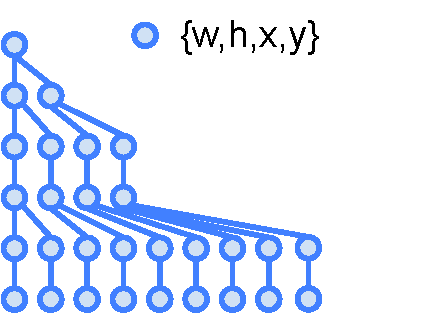
\includegraphics[trim=0 0 0 0,clip,width=0.3\columnwidth]{chapter6/bfslayouttree} } 
 \subfloat[\textbf{Tree Representation}]{\label{fig:bfstraversal:repmem}  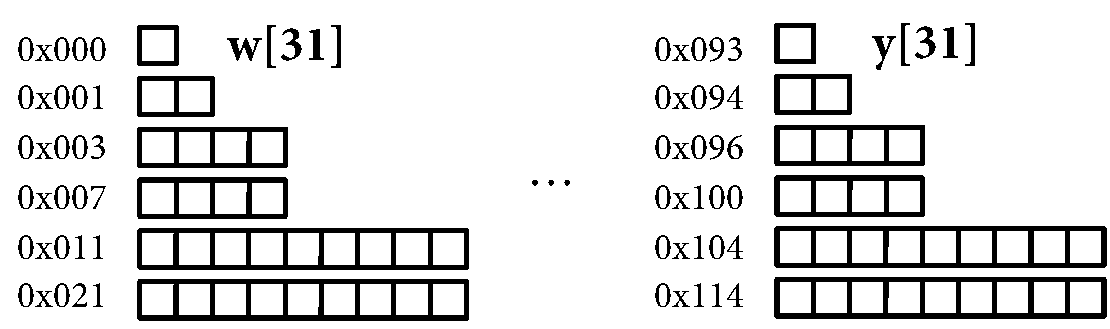
\includegraphics[trim=0 0 0 0,clip,width=0.6\columnwidth]{chapter6/bfslayoutmem} } 
\caption{\textbf{SIMD tree traversal as level-synchronous breadth-first iteration with corresponding structure-split data representation.}}
\label{fig:bfstraversal}
\end{figure}

The na\i{v}e tree traversal schedule is to sequentially iterate one level of the tree at a time and  traverse the nodes of a level in parallel. A parallel preorder traversal starts on the root node's level and then proceeds downwards, while a postorder traversal starts on the tree fringe and moves upwards (Figure~\ref{fig:bfstraversal}~\ref{fig:bfstraversal:code}). Our MIMD implementation, in contrast, allows one processor to compute on a different tree level than another active processor. In data visualizations, we empirically observed that most of the nodes on a level will dispatch to the same layout instructions, so our na\i{v}e traversal schedule avoids instruction divergence.

The level-synchronous traversal pattern eliminates many divergent memory accesses by using a corresponding data representation. Adjacent nodes in the schedule are collocated in in memory. Furthermore, individual node attributes are stored in \emph{column} order through a array-of-structure to structure-of-array conversion. The conversion collocates individual attributes, such as the width attribute of one node being stored next to the width attribute of the node's sibling (Figure~\ref{fig:bfstraversal:repmem}). The index of a node in a breadth-first traversal of the tree is used to perform a lookup in any of the attribute arrays. The benefit this encoding is that, during SIMD  layout of several adjacent nodes, reads and writes are coalesced into  bulk reads and writes. For example, if a layout pass adds a node's padding to its width, several contiguous paddings and several contiguous widths will be read, and the sum will be stored with a contiguous write. Such optimizations are crucial because the penalty of non-coalesced access is high and, for layout, relatively few computations occur between the reads and writes.

Full implementation of the data representation poses several subtleties. 
\begin{itemize}
\item \textbf{Level representation.} To eliminate traversal overhead, a summary provides the index of the first and last node on each level of a tree. Such a summary provides  data range information for launching the parallel kernels that evaluate the nodes of a level as well as the information for how to proceed to the next level.
\item \textbf{Edge representation.} A node may need multiple named lists of children, such as an HTML table with a header, footer, and an arbitrary number of rows. We encode the table's edges as 3 global arrays of offsets: header, footer, and first-row. To support iterating across rows, we also introduce a 4th array to encode whether a node is the last sibling. Thus, any named edge introduces a global array for the offset of the pointed-to node, and for iteration, a shared global array reporting whether a node at a particular index is the end of a list.
\item \textbf{Memory compression.} Allocating an array the size of the tree for every type of node attribute wastes memory. We instead statically compute the maximum number of attributes required for any type of node, allocate an array for each one, and map the attributes of different types of nodes into different arrays. For example, in a language of HBox nodes as Circle nodes who have attributes 'r' and 'angle', 4 arrays will be allocated. The HBox requires an array for each of the attributes 'w', 'h', 'x', and 'y' while the Circle nodes only require two arrays. Each node has one type, and if that that type is HBox, the node's entry in the first array will contain the 'w' attribute. If the node has type Circle, the node's entry in the first entry will contain the 'r' attribute.
\item \textbf{Tiling.} Local structural mutations to a tree such as adding or removing nodes should not force global modifications. As most SIMD hardware has limited vector lengths (e.g., 32 elements wide), we split our representation into blocks. Adding nodes may require allocation of a new block and reorganization of the old and new block. Likewise, after successive additions or deletions, the overall structure may need to be compacted. Such techniques are standard for file systems, garbage collectors, and databases.
\end{itemize}


In summary, our basic SIMD tree traversal schedule and data representation descend from the approach of NESL [[CITE]] and Data Parallel Haskell [[CITE]]. Previous work shows how to generically convert a tree of structures into a structure of arrays. Those approaches do not support statically unbounded nesting depth (i.e., tree depth), but our system supports arbitrary tree depth because our transformation is not as generic.  

A key property of all of our systems, however, is that the structure of the tree is fixed prior to the traversals.  In contrast, for example, parallel breadth-first traversals of graphs will dynamically find a minimum spanning tree [[CITE]]. Such dynamic alternatives incur unnecessary overheads when performing a sequence of traversals and sacrifice memory coalescing opportunities. Layout is often a repetitive process, whether due to multiple tree traversals for one invocation or an animation incurring multiple invocations, so costs in creating an optimized data representation and schedule are worth paying.

\section{Input-dependent Clustering for SIMD Evaluation}
Once the tree is available, we automatically optimize the schedule for traversing a tree level in a way that avoids instruction divergence. Our insight is that we can cluster tasks (nodes) based on node attributes that influence control flow. We match the data layout to the new schedule, and optimize the clustering process to prevent the planning overhead to outweigh its benefit. The overall optimization can be thought of an extension to loop unswitching where the predicate is input-dependent and a sorting prepass guarantees that subintervals will branch identically.

\begin{figure}
\subfloat{  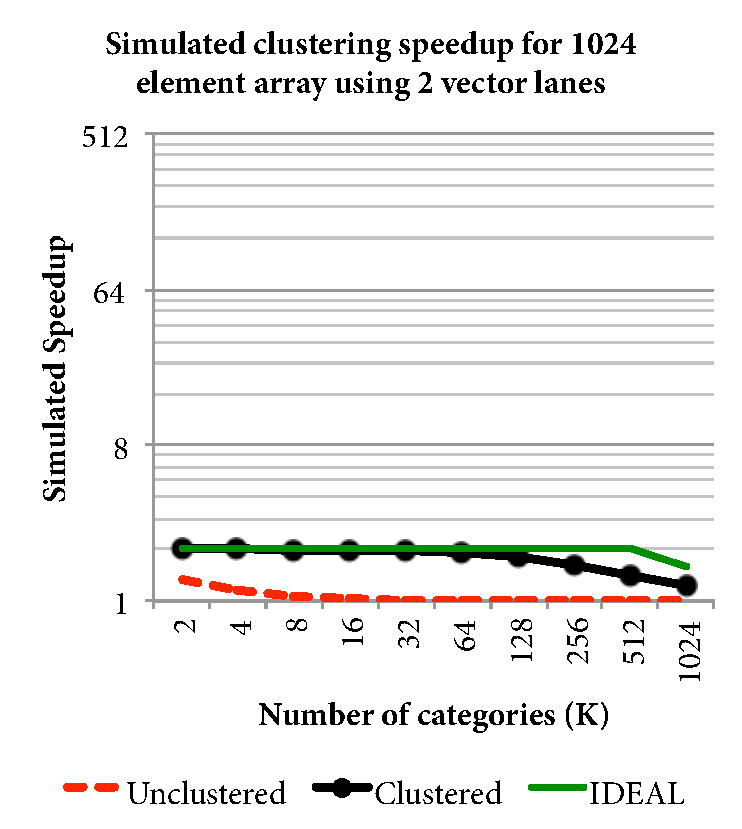
\includegraphics[trim=0 0 0 0,clip,width=0.32\columnwidth]{chapter6/simulatedclusteringspeedup/simulatedclusteringspeedup-1} }
\subfloat{  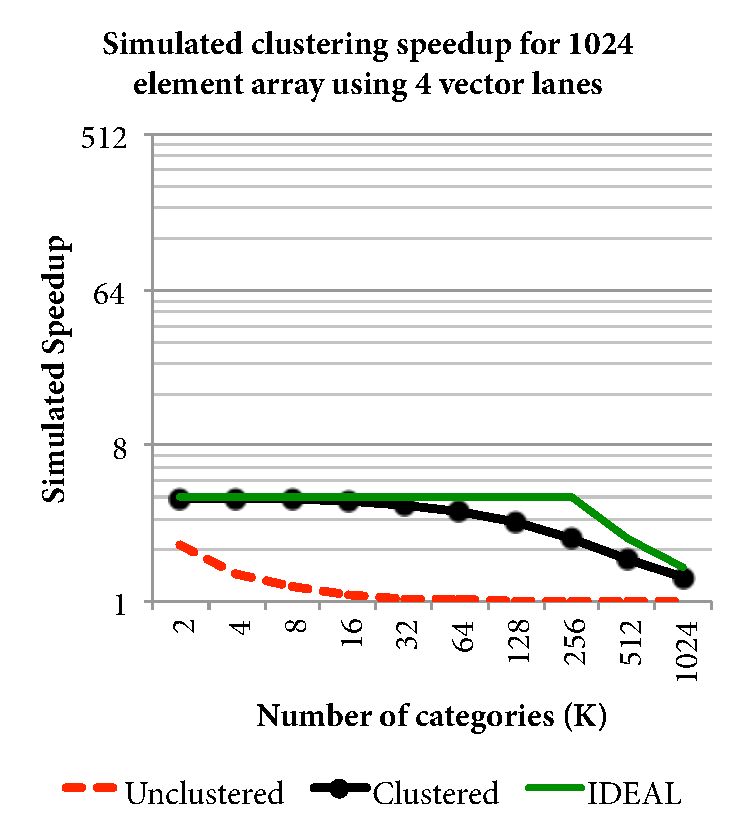
\includegraphics[trim=0 0 0 0,clip,width=0.32\columnwidth]{chapter6/simulatedclusteringspeedup/simulatedclusteringspeedup-2} }
\subfloat{  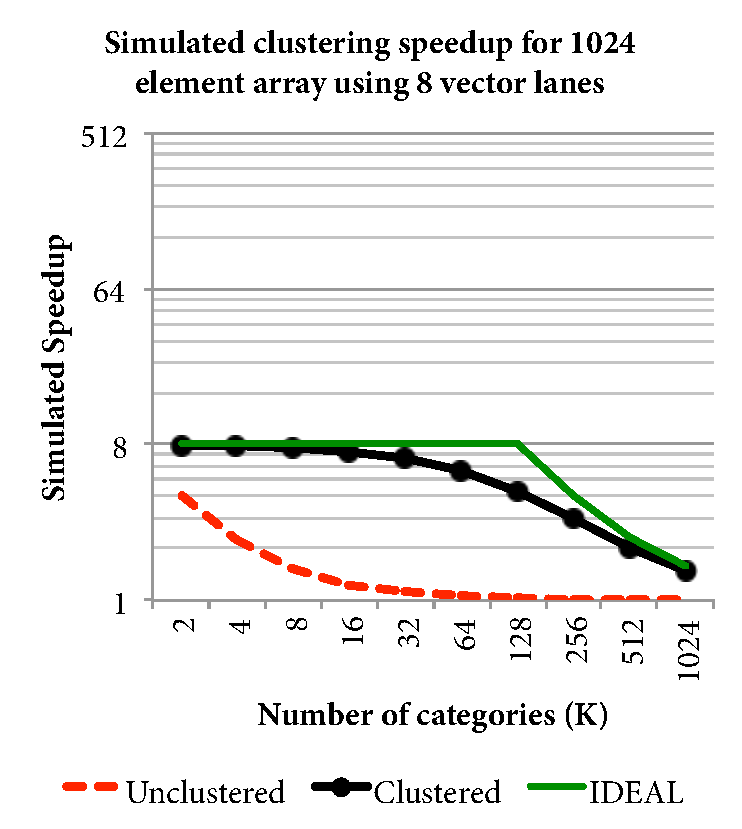
\includegraphics[trim=0 0 0 0,clip,width=0.32\columnwidth]{chapter6/simulatedclusteringspeedup/simulatedclusteringspeedup-3} } \\
\subfloat{  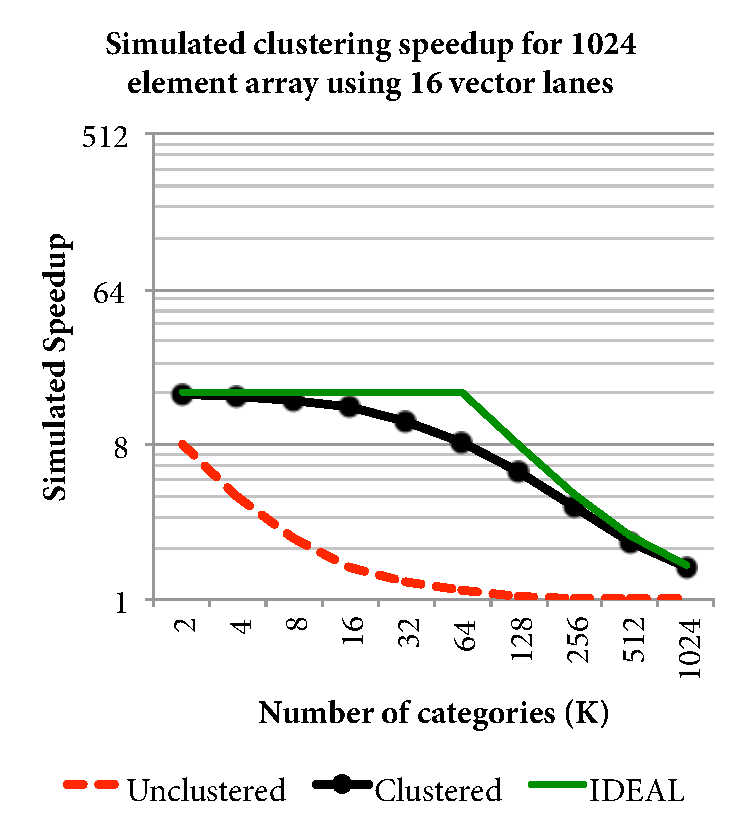
\includegraphics[trim=0 0 0 0,clip,width=0.32\columnwidth]{chapter6/simulatedclusteringspeedup/simulatedclusteringspeedup-4} }
\subfloat{  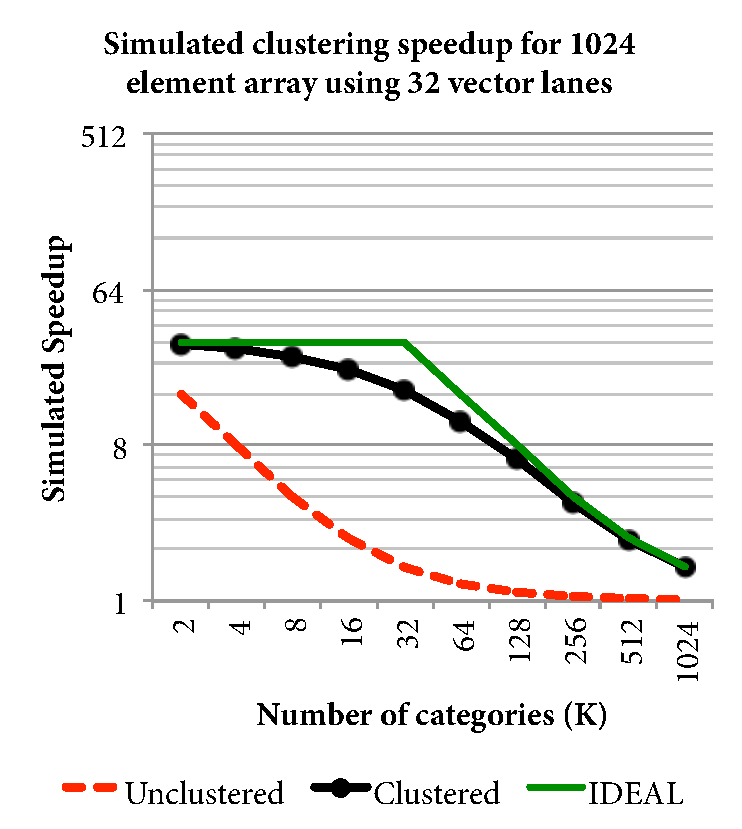
\includegraphics[trim=0 0 0 0,clip,width=0.32\columnwidth]{chapter6/simulatedclusteringspeedup/simulatedclusteringspeedup-5} }
\subfloat{  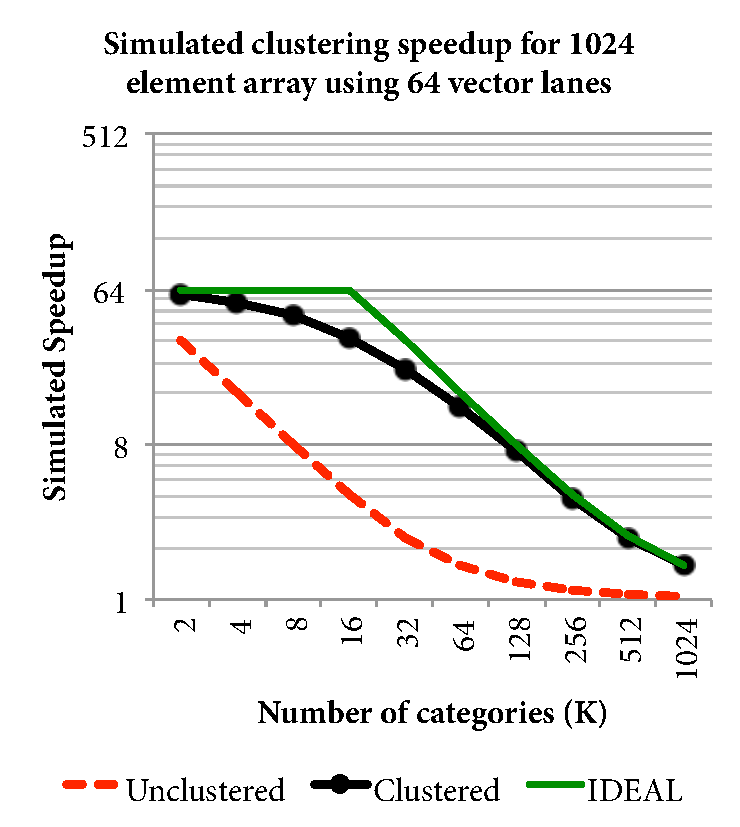
\includegraphics[trim=0 0 0 0,clip,width=0.32\columnwidth]{chapter6/simulatedclusteringspeedup/simulatedclusteringspeedup-6} } \\
\subfloat{  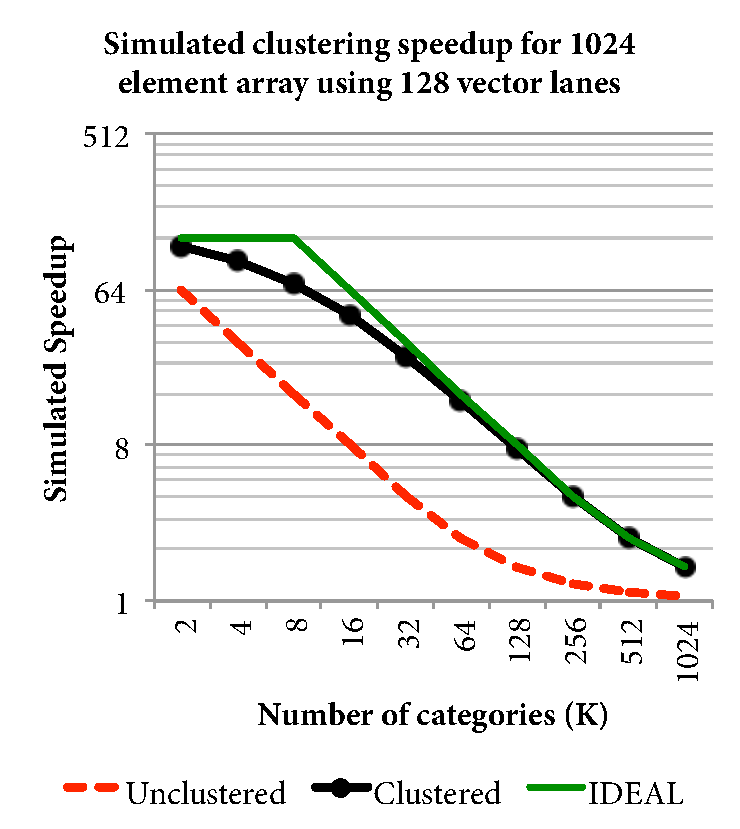
\includegraphics[trim=0 0 0 0,clip,width=0.32\columnwidth]{chapter6/simulatedclusteringspeedup/simulatedclusteringspeedup-7} }
\subfloat{  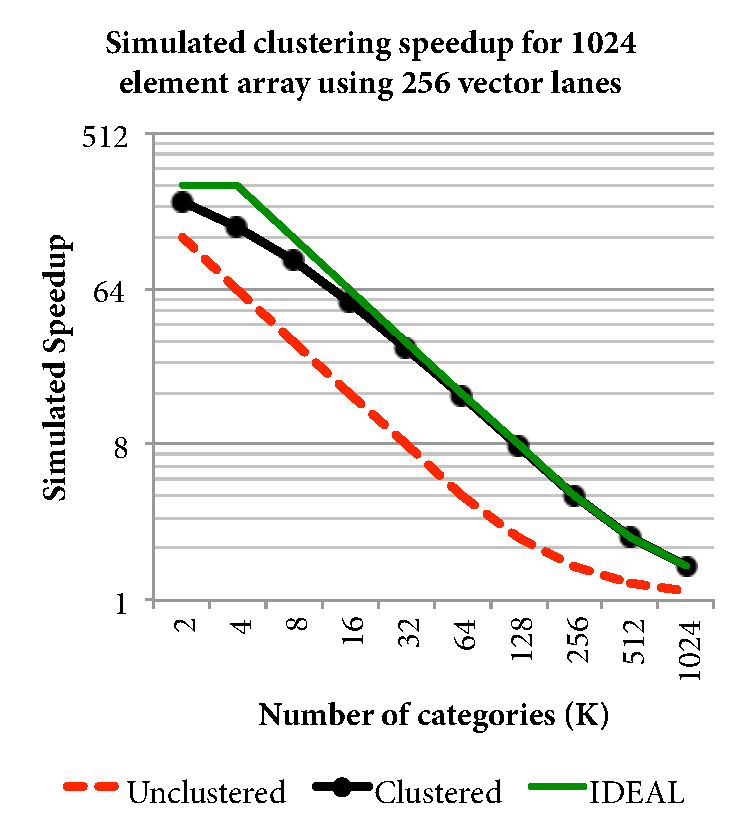
\includegraphics[trim=0 0 0 0,clip,width=0.32\columnwidth]{chapter6/simulatedclusteringspeedup/simulatedclusteringspeedup-8} }
\subfloat{  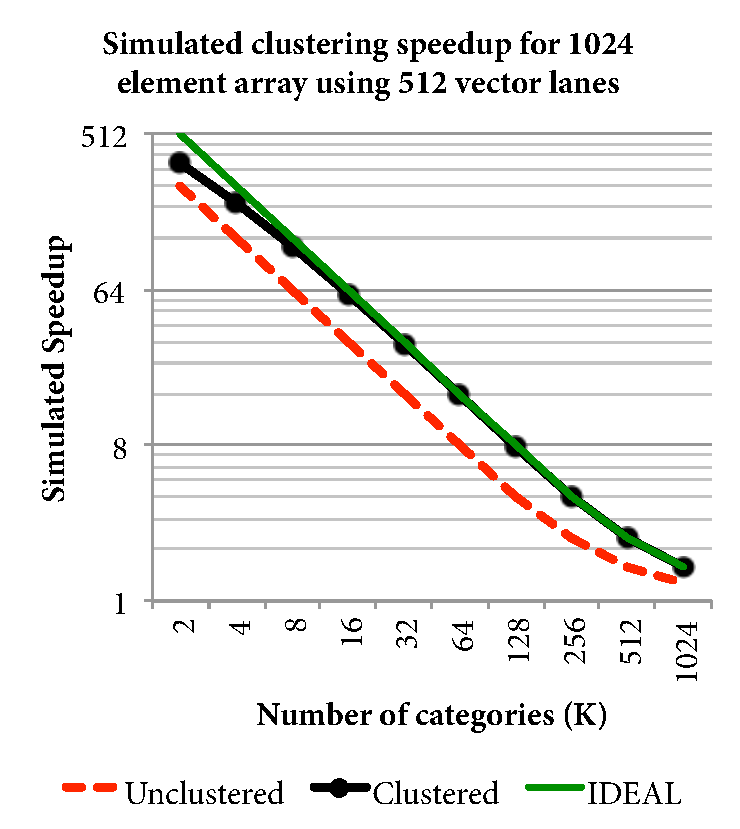
\includegraphics[trim=0 0 0 0,clip,width=0.32\columnwidth]{chapter6/simulatedclusteringspeedup/simulatedclusteringspeedup-9} } \\
\caption{\textbf{blah}}
\label{fig:simulatedclusteringspeedup}
\end{figure}





\subsection{The Problem}
The problem we address stems from layout being a computation where the instructions for each node are heavily input dependent. The intuition can be seen in contrasting the visual appearance of a webpage vs. a data visualization. Different parts of a webpage look quite different from one another, which suggests sensitivity to values in the input tree, while a visualization looks self-similar and thus does not use widely different instructions for different nodes.  For an example of divergence, an HBox's width is the sum of its children widths, while a VBox's is their maximum. The visit to a node (Figure~\ref{fig:compiled}) will diverge in instruction selection based on the node type.  

We ran a simulation to measure the performance cost of the divergence. Assuming a uniform distribution of types of nodes in a level, as the number of types of nodes go up ($K$), the probability that all of the nodes in a group share the same instructions drops exponentially. Figure~\ref{fig:simulatedclusteringspeedup} shows the simulated speedup for SIMD evaluation over a tree level of 1024 nodes on computer architectures with varying SIMD lengths. The x axis of each chart represents the number of types and the y axis is the speedup. As the number of choices increase, the benefit of the na\i{v}e breadth-first schedule (red line) decreases. It is far from the ideal speedup, which we estimated as a function of the SIMD length of the architecture (maximal parallel speedup, contributing the horizontal portion of the green lines) and the expected number of different categories (mandatory divergences, contributing the diagonal portion). 

\subsection{Code Clustering}
Our solution is to cluster nodes of a level based on the values of attributes that influence the flow of control. SIMD evaluation of the nodes in a cluster will be free of instruction divergence. Furthermore, by changing the data representation to match the clustered schedule, memory accesses will also be coalesced. We first focus on applying the clustering transformation to the code.



\newsavebox{\bfsClusteredVisitor}
\begin{lrbox}{\bfsClusteredVisitor}% Store first listing
\begin{lstlisting}[mathescape,language=C++,morekeywords={spawn,join,reverse,parallel_for}]
void parPreClustered(void (*visit)(Prod &), List<List<Array<Prod>>>  &levels) {
  for (List<Prod> level in levels)
  	for (Array<Prod> cluster in level)
  		parallel_for (Prod p in cluster)
			visit(p)
}
\end{lstlisting}
\end{lrbox}

\begin{figure}
 \usebox{\bfsClusteredVisitor}  
\caption{\textbf{Clustered parallel preorder traversal.}}
\label{fig:clusteredeval}
\end{figure}


\newsavebox{\clusterUnswitchA}
\begin{lrbox}{\clusterUnswitchA}% Store first listing
\begin{lstlisting}[mathescape]
Prod firstProd = cluster[0]
parallel_for (prod in Cluster) {
  switch (firstProd.type) {
    case S $\rightarrow$ HBOX:  break;
    case HBOX $\rightarrow$ $\epsilon$:
      HBOX.w = input(); 
      HBOX.h = input(); 
      break;
    case HBOX $\rightarrow$ HBOX$_1$ HBOX$_2$:
      HBOX$_0$.w = HBOX$_1$.w + HBOX$_2$.w;
      HBOX$_0$.h = MAX(HBOX$_1$.h, HBOX$_2$.h);
      break;
  }
 }
\end{lstlisting}
\end{lrbox}

\newsavebox{\clusterUnswitchB}
\begin{lrbox}{\clusterUnswitchB}% Store first listing
\begin{lstlisting}[mathescape]
Prod firstProd = cluster[0]
  switch (firstProd.type) {
    case S $\rightarrow$ HBOX:  break;
    case HBOX $\rightarrow$ $\epsilon$:
      parallel_for (prod in Cluster) {
          HBOX.w = input(); 
          HBOX.h = input();
     }
      break;
    case HBOX $\rightarrow$ HBOX$_1$ HBOX$_2$:
      parallel_for (prod in Cluster) {
        HBOX$_0$.w = HBOX$_1$.w + HBOX$_2$.w;
        HBOX$_0$.h = MAX(HBOX$_1$.h, HBOX$_2$.h);
      }
      break;
  }
 }
\end{lstlisting}
\end{lrbox}



\begin{figure}
\subfloat[\textbf{Clustered dispatch.}]{ \usebox{\clusterUnswitchA} } 
\subfloat[\textbf{Unswitched dispatch}.]{\usebox{\clusterUnswitchB} } 
\caption{\textbf{Loop transformations to exploit clustering for vectorization.}}
\label{fig:clusteringunswitching}
\end{figure}


Figure~\ref{fig:clusteredeval} shows the clustered evaluation variant of the MIMD $parPre$ traversal of Figure~\ref{fig:hboxall}. The traversal schedule is different because the order is based on the clustering rather than breadth-first index. Changing the order is safe because the original loop was parallel with no dependencies between elements.  Computing over clusters guarantees that all calls to a visit dispatch function in the parallel inner loop (e.g., of $visit1$) will branch to the same switch statement case. This modified schedule avoids instruction divergence. 

Our loop transformation can be understood as a use of loop unswitching, which is a common transformation for improving parallelization. Loop unswitching lifts a conditional out of a loop by duplicating the  loop inside of both cases of the conditional. Clustering establishes the invariant of being able to inspect the first item of a collection sufficing for performing unswitching for a loop over all of the items. Figure~\ref{fig:clusteringunswitching} separates our transformation of $visit1$ (Figure \ref{fig:hboxall}) into using the same exemplar for the dispatch and then loop unswitching.

Clustering is with respect to input attributes that influence control flow, which may be more than the node type. For example, in our parallelization of the C3 layout engine, we found that the engine author combined the logic of multiple box types into one visit function because the variants shared a lot of code. He instead used multiple node flags to guide instruction selection. Both the node type and various other node attributes influenced control flow, and therefore our clustering condition was on whether they were all equal. Using all of the attributes led to too granular of a clustering condition, so we manually tuned the choice of attributes.

\subsection{Data Clustering}
The data representation should be modified to match the clustering order. The benefit is coalesced memory accesses, but overhead costs in performing the clustering should be considered.

Our algorithm matches the data representation order to the schedule by placing nodes of a cluster into the same contiguous array. Parallel reads and are coalesced, such as the inspection of the node type for the visit dispatch. Parallel writes are likewise coalesced.

Reordering data is expensive as all of the data is moved. In the case of our data visualization system, we can avoid the cost because the data is preprocessed on our server. For webpage layout, the client performs clustering, which we optimize enough such that the cost is outweighed by the subsequent performance improvements.

We optimize reordering with a simple parallel two-pass technique. The first pass traverses each level in parallel to compute the cluster for each node and tabulate the cluster sizes for each tree level. The second pass again traverses each level in parallel, and as each node is traversed, copies it into the next free slot of the appropriate cluster. Even finer-grained parallelization is possible, but this algorithm was sufficient for lowering reordering costs enough to be amortized.

\subsection{Nested Clustering}
Clustering can also be used to address divergences induced by computations over neighboring nodes. They avoidable irregularities can take several forms:

\begin{itemize}
\item \textbf{Branches.} For the case of webpage layout, we saw cases where attributes of the parent node or children node influence instruction selection, such as whether to include a child node in a width computation. The properties can be included in the clustering condition to eliminate the corresponding instruction divergences. 

\item \textbf{Load imbalance in loops.} One node may have no children while another may have many. If the layout computation involves a loop, SIMD evaluation will perform the two loops in lock-step. Thus, as the nodes have different amounts of children, the SIMD lanes devoted to the first child will not be utilized: this is a load balancing problem. The number of children can be included in the clustering condition to eliminate load imbalance.

\item \textbf{Random memory access in loops.} A further issue with lock-step loops over child nodes is memory divergence. A breadth-first layout would provide strided memory access, but if each level is clustered, the locations of a node's children may be random without further aid. We found a \emph{nested} solution where \emph{subtrees} are assigned to clusters. Instead of just associating nodes of a level with a cluster, our algorithm then treats the nodes of a cluster as roots. It recursively expands a subtree such that all of the cluster nodes share it (with respect to the attributes influencing control flow). The data layout follows the nested clustering, so parallel memory accesses to the children of nodes will be coalesced. 
\end{itemize}

Each of these clusterings introduce an invariant for a cluster for optimizing performance within that cluster. However, the clustering condition is more discriminating.  Cluster sizes may decrease, which would  significantly decrease  performance if cluster size shrinks below vector length size. Our evaluation explores these options in practice.



\section{Evaluation}






\begin{table}[t]
\center
\begin{tabular}{l|c|c|c|c| c | c | c}
~  &\multicolumn{4}{c|}{\textbf{Total speedup}} & \multicolumn{3}{c}{\textbf{Parallel speedup}}\\
~  &\multicolumn{4}{c|}{Cores} & \multicolumn{3}{c}{Cores}\\
{\small \textbf{Configuration}} & 1 & 2 & 4 & 8 & 2 & 4 & 8\\ [0.5ex] \hline \hline
TBB, \code{server} & 1.2x & 0.6x & 0.6x & 1.2x & 0.5x & 0.5x & 1.0x \\ \hline
FTL, \code{server} & 1.4x & 2.4x & 5.2x & 9.3x & 1.8x & 3.8x & 6.9x \\ 
FTL, \code{laptop} & 1.4x & 2.1x & & & 1.6x &     &  \\ 
FTL, \code{mobile} & 1.3x & 2.2x & & & 1.7x &     &  \\ 
\end{tabular}
\caption{\textbf{Speedups and strong scaling across different backends (Back) and hardware}. Baseline is a sequential traversal with no data layout optimizations. FTL is our multicore tree traversal library. Left columns show total speedup (including data layout optimizations by our code generator) and right columns show just parallel speedup. Server = Opteron 2356, laptop = Intel Core i7, mobile = Atom 330.}
\label{tab:diffhw}
\end{table}

\subsection{MIMD Data Representation and Scheduling Optimizations}
By statically exposing traversal structure (e.g., \sched{parPre}) to our code generators, we observe sequential and parallel speedups. We separately evaluate the importance of the data representation optimizations from the scheduling ones on random 500-1000 node documents in the \hlangpp{} language. Finally, we examine the parallel benefit on webpages.


We first evaluate the perform of our task scheduler (FTL in Table~\ref{tab:diffhw}).  Our comparison point is Intel's TBB~\cite{inteltbb} dynamic task scheduler that performs work stealing~\cite{cilk}, which was the most efficient third-party work stealing library that we tried. We included our data layout optimizations in all calculations because, without them, we saw no speedup.  TBB causes slowdowns until achieving no cost (nor benefit) at 8 cores. Our insight is that it suffered from high overheads: switching to scheduling tiles by using our optimized data representation improved performance. Our semi-static working stealing scheduler, however, achieved a 6.9X speedup on 8 cores. We did not see significant further speedups for higher core counts, and hypothesize that it is due to the socket jump. We experimented with other schedulers, such as a simple for-loop over tiles near the fringe of the tree, but the achieved 2X speedup is much lower than the 6.9X of our semi-static work stealer.


Data representation was key to achieving parallel speedups. It achieved 1.2X-1.4X speedups for sequential processing (Table~\ref{tab:diffhw}). However, on 4 cores, it improved performance from 2.8X without data representation optimizations to 5.2X when using them. The difference is 1.9X: our data representation optimizations both complement and improve scheduling optimizations. Without them, parallel performance was poor.

\begin{table}[t]
\center
\begin{tabular}{l|l| c | c | c}
~ & & \multicolumn{3}{c}{\textbf{Parallel speedup}}\\
~ & & \multicolumn{3}{c}{Cores}\\
\textbf{Backend} & Input & 2 & 4 & 8\\ [0.5ex] \hline \hline
TBB & {Wikipedia} &  1.5x & 1.6x & 1.2x \\
TBB & {xkcd Blog} &  1.5x & 1.8x & 1.2x \\ \hline
FTL & {Wikipedia} &  1.6x & 2.8x & 3.2x \\
FTL & {xkcd Blog} &  1.5x & 2.3x & 3.1x \\ 
\end{tabular}
\caption{\textbf{Parallel CSS layout engine}. Run on a 2356 Opteron.}
\label{fig:cssperf}
\end{table}

Table~\ref{fig:cssperf} shows the parallel speedup on running our 9 pass layout engine for two popular web pages that render faithfully with it: Wikipedia and the XKCD blog. Note that the benchmarks do \emph{not} include sequential speedups. The best performance of TBB was a 1.8X speedup on 4 cores, and its speedup on 8 cores was 1.2X. In comparison, our scheduler achieved 2.8X on 2 cores and 3.2X on 8X. Our insight as to why we did not see further benefits is overheads. Across our benchmarks, we generally saw speedups when sequential traversals took longer than a certain amount, but because so many traversals are used for CSS, enough of them are small enough that we do not expect strong scaling. Our intuition is that either a full layout engine is complicated enough that the sequential cost of each traversal will be higher than in our prototype, or even more aggressive data representation optimizations should be performed. As is, we have demonstrated significant 3X+ speedups on real workloads from just the parallelization.


\begin{figure}
\centering
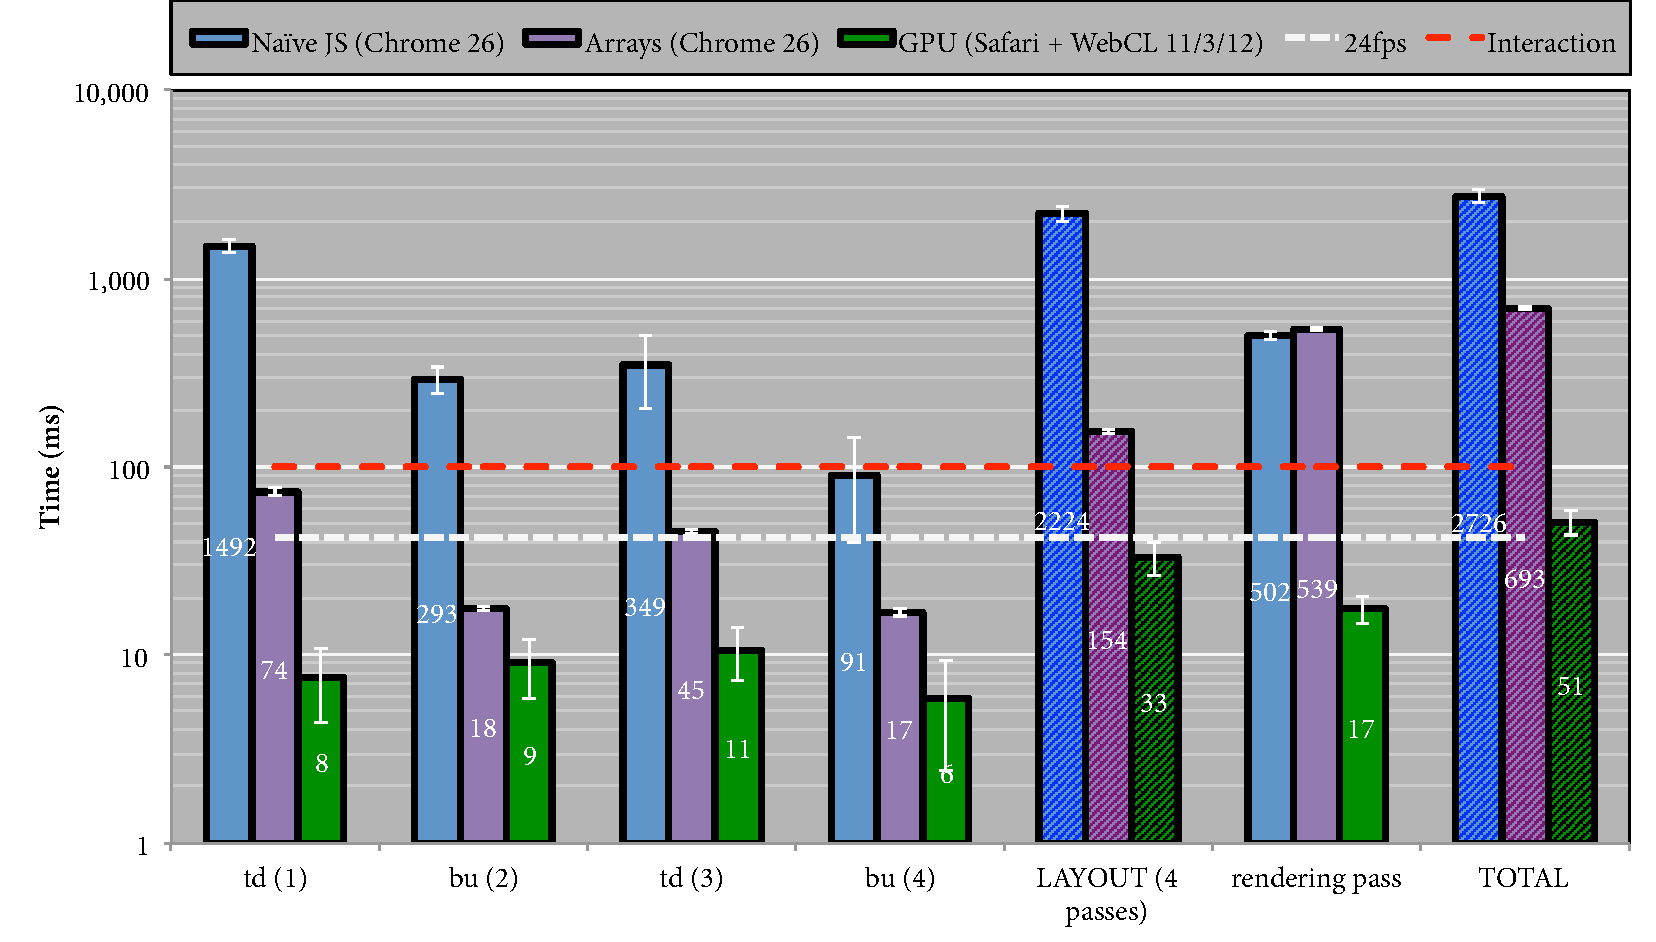
\includegraphics[trim=0 0 0 0,clip,width=1.0\columnwidth]{chapter6/gpuspeedup}
\caption{\textbf{Sequential and Parallel Benefits of Breadth-First Layout and Staged Allocation.} Allocation is merged into the 4th stage and buffer indexing and tessellation form the rendering pass. JavaScript variants use HTML5 canvas drawing primitives while WebCL does not include WebGL painting time ($<$ 5ms). Thin vertical bars indicate standard deviation and horizontal bars show deadlines for animation and hand-eye interaction.}
\label{fig:treemapjsgpu}
\end{figure}


\subsection{Baseline SIMD Speedups (GPU)}
We evaluate the sequential and parallel performance benefits of our baseline breadth-first layout.   For an animation to achieve 24fps, the time spent to process a frame should not exceed 42ms, and for eye-hand interactions, 100ms (10fps). We examine the case of a 5 pass treemap that supports live filtering over 100,000 data points. The first 3 passes are purely devoted to layout, the 4th pass includes layout computations and allocation requests, and the 5th pass propagates buffer indices and performs tessellation. 

We compare 3 backends for our compiler: canonical JavaScript (a tree of nodes), JavaScript over our structure-split breadth-first tree layout (and with typed arrays~[[CITE]]), and WebCL for the GPU.  The first two variants invoke HTML5 canvas drawing primitives, while the last invokes WebGL (GPU) painting primitives over vertex buffers computed in the rendering pass. The time for WebGL painting calls are not shown, but they take less than 5ms. Each variant is repeated 15 times on a 4 core 2012 2.66GHz Intel Core i7 with 8 GB memory and a 1024 MB NVIDIA GeForce GT 650M graphics card.

We first examine  the significant sequential benefits.The first 4 groups of columns in Figure~\ref{fig:treemapjsgpu} shows the average time spent on different layout passes and the 6th on the pass for buffer index computation and tessellation. Performing compiler optimizations enables a 14X sequential speedup on layout in the Chrome web browser. No speedup is observed in the rendering pass because the time is dominated by HTML5 canvas calls. We hypothesize part of the sequential benefit is related to our clustering optimization: all of the nodes in a level have the same type, so implicit optimizations such as branch prediction should perform better. Finally, we note that while sequential layout time is a magnitude too slow for real-time animation, our prototype is within 54ms for real-time interaction (ignoring rendering).

Parallel speedups are also significant. WebCL (GPU) evaluation of layout is 5X faster than sequential. The impact of compiling JavaScript vs. C (WebCL) on the benchmark is unclear: JavaScript is generally a magnitude slower than native code, except the runtime WebCL compiler is not running at high optimization levels. The benefits for parallel computation of the buffer indices and tessellation is much more clear: the speedup is 31X. 

\begin{figure}
\centering
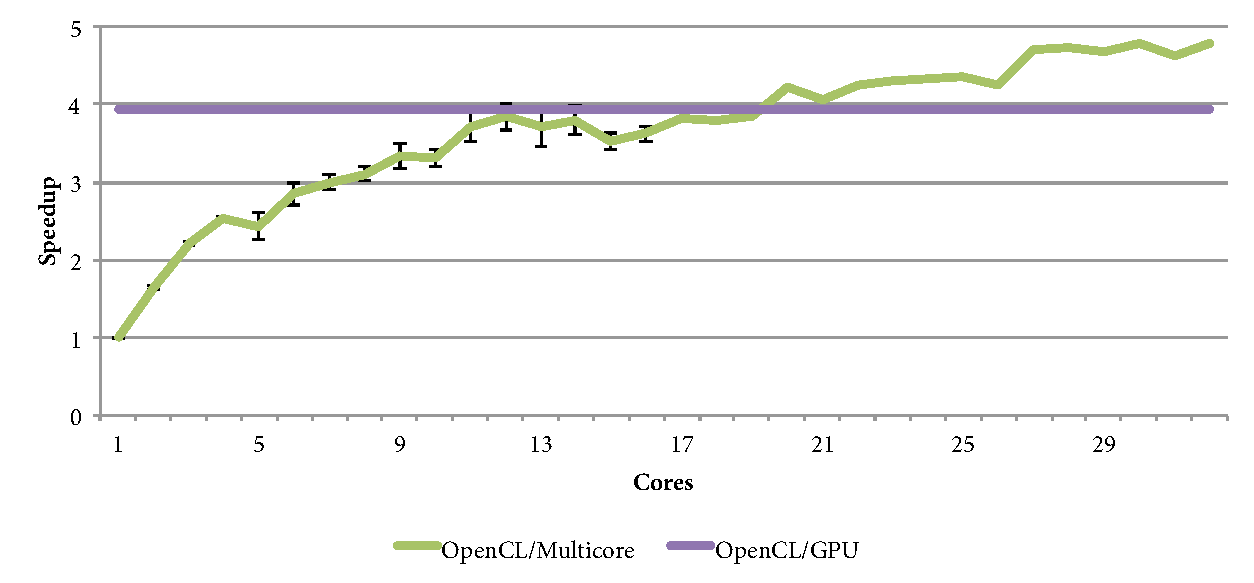
\includegraphics[trim=0 0 0 0,clip,width=1.0\columnwidth]{chapter6/gpuvscpu}
\caption{\textbf{Multicore vs. GPU Acceleration of Layout.} Benchmark on an early version of the treemap visualization and does not include rendering pass.}
\label{fig:cpuvsgpu}
\end{figure}

To better understand the benefit of parallelization, we compared running the layout traversals using multicore vs. GPU acceleration (Figure~\ref{fig:cpuvsgpu}) for an early prototype of the layout traversals. Both use breadth-first traversals compiled with OpenCL, except differ on the hardware target. We see that a server-grade multiprocessor (32-core AMD Opteron 2356) can outperform a laptop GPU, but the comparison is unfair in terms of power consumption. TODO compare power ratings.


Ultimately, when the sequential and parallel optimizations are combined, we see an end-to-end speedup of 54X. It is high enough such that it enables real-time animation for our data set, not just real-time user interaction.


\subsection{SIMD Clustering}
We evaluate several aspects of our clustering approach. First, we examine applicability to various visualizations. Second, we evaluate the speed and performance benefit. Clustering provides invariants that benefit more than just vectorization, so we distinguish sequential vs. parallel speedups. Finally, there are different options in what clusters to form, so for each stage of evaluation, we compare impact.

\begin{figure}
\centering
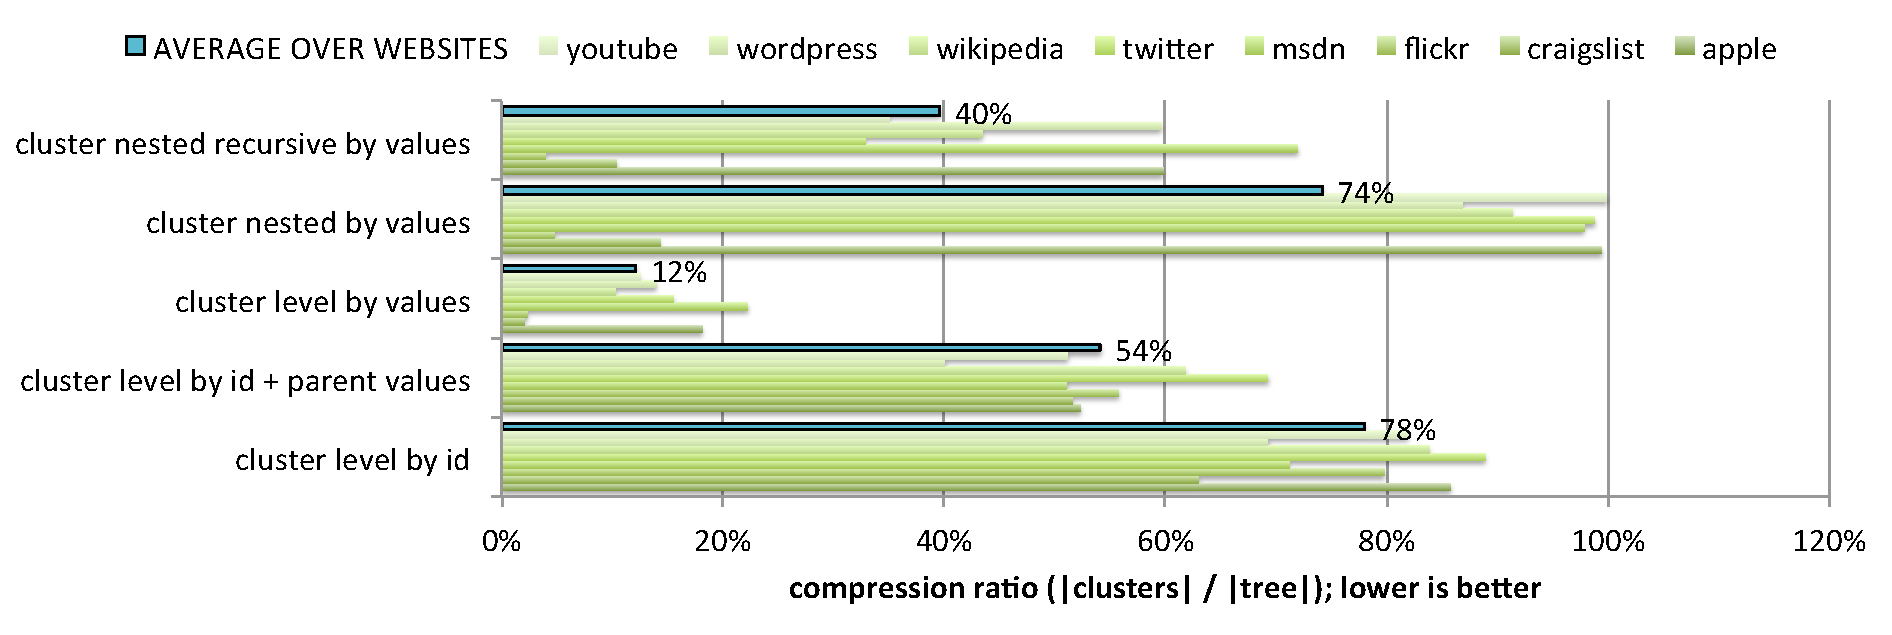
\includegraphics[trim=0 0 0 0,clip,width=1.0\columnwidth]{chapter6/csscompression}
\caption{\textbf{Compression ratio for different CSS clusterings.} Bars depict compression ratio (number of clusters over number of nodes). Recursive clustering is for the reduce pattern, level-only for the map pattern. ID is an identifier set by the C3 browser for nodes sharing the same style parse information while value is by clustering on actual style field values.}
\label{fig:csscompression}
\end{figure}




\subsubsection{Applicability}


We examined idealized speedup for several workloads:

\begin{itemize}

\item \textbf{Synthetic.} For a controlled synthetic benchmark, we simulated the effect of increasing number of clusters on speedup for various SIMD architectures.  Our simulation assumes perfect speedups for SIMD evaluation of nodes run together on a SIMD unit. The ideal speedup is a function of the minimum of the SIMD unit's length (for longer clusters, multiple SIMD invocations are mandatory) and the number of clusters (at least one SIMD step is necessary for each cluster).   Figure~\ref{fig:simulatedclusteringspeedup} shows, for architectures of different vector length, that the simulated speedup from clustering (solid black line with circles) is close to the ideal speedup (solid green line).

\item \textbf{Data visualization.} For our data visualizations, we found that, across the board, all of the nodes of a level shared the same type. For example, our visualization for multiple line graphs puts the root node on the first level, the axis for each line graph on the second level, and all of the actual line segments on the third level. 

\item \textbf{CSS.} We analyzed potential speedup on webpages. Webpages are a challenging case because an individual webpage features high visual diversity, with popular sites using an average of 27KB of style data per page.~\footnote{https://developers.google.com/speed/articles/web-metrics}. We picked 10 popular websites from the Alexa Top 100 US websites that rendered sufficiently correctly in the C3~[[CITE]] web browser. It was also challenging in practice because it required clustering based on individual node attributes, not just the node type.

Figure~{fig:csscompression} compares how well nodes of a webpage can be clustered. It reports the \emph{compression ratio}, which divides the number of clusters by the number of nodes. Sequential execution would assign each node to its own cluster, so the ratio would be 1. In contrast, if the tree is actually a list of 100 elements, and the list can be split into 25 clusters, the ratio would be 25\%. Assuming infinite-length vector processors and constant-time evaluation of a node, the compression ratio is the exact inverse of the speedup. A ratio of 1 leads to a 1X speedup, and a compression ratio of 25\% leads to a 4X speedup.

Clustering each level by attributes that influence control flow achieved a 12\% compression ratio (Figure~{fig:csscompression}): an 8.3X idealized speedup. When we strengthened the clustering condition to enforce stronger invariants in the cluster, such as to consider properties of the parent node, the ratio quickly worsened. Thus, we see that our basic approach is promising for websites on modern subword-SIMD instruction sets, such as a 4-wide SSE (x86) and NEON (ARM), and the more recent 8-wide AVX (x86). Even longer vector lengths are still beneficial because some clusters were long. However, eliminating all divergences requires addressing control flows influenced by attributes of node neighbors, which leads to poor compression ratios. Thus, we emphasize that 8.3X is an upper bound on the idealized speedup: not all branches in a cluster are addressed.
\end{itemize}

Empirically, we see that clustering is applicable to CSS, and in the case of our data visualizations, unnecessary. Vectorization limit studies based on analyzing dynamic data dependencies from program traces suggest that general programs can be much more aggressively vectorized, so clustering may be the beginning of one such approach~[[CITE]].




\begin{figure}
\centering
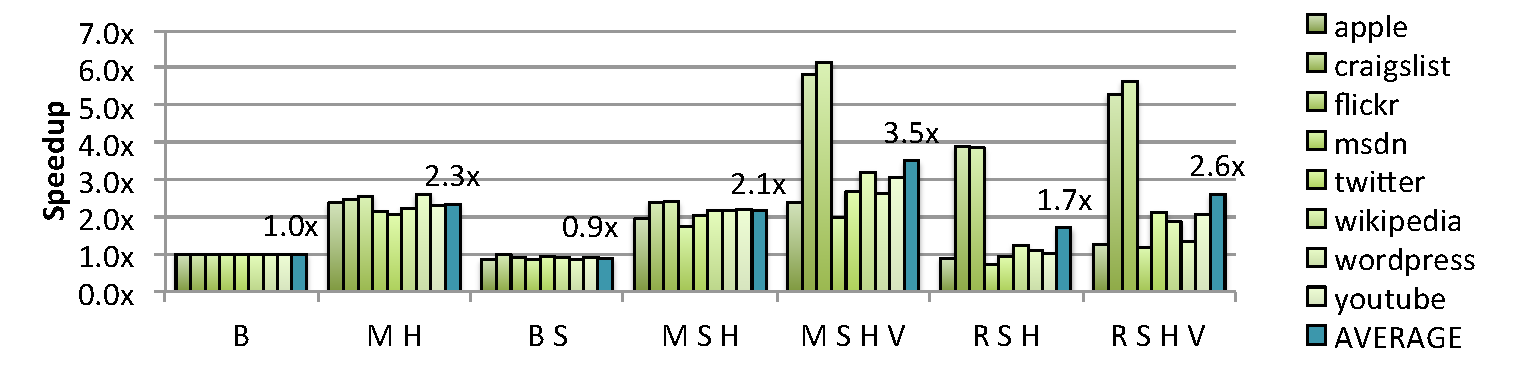
\includegraphics[trim=0 0 0 0,clip,width=1.0\columnwidth]{chapter6/cssspeedup4}
B =breadth first, S = structure splitting, M = level clustering, R = nested clustering, H = hoisting, V = SSE 4.2 
\caption{\textbf{Speedups from clustering on webpage layout.} Run on a 2.66GHz Intel Core i7 (GCC 4.5.3 with flags -O3 -combine -msse4.2) and does not preprocessing time.
}
\label{fig:cssspeedup}
\end{figure}

\subsubsection{Speedup}
We evaluate the speedup benefits of clustering for webpage layout. We take care to distinguish sequential benefits from parallel, and of different clustering approaches. Our implementation was manual:  we examine optimizing one pass of the C3~[[CITE]] browser's CSS layout engine that is responsible for computing intrinsic dimensions. The C3 browser was written in C\#, so we wrote our optimized traversal in C\+\+ and pinned the memory for shared access.  We use a breadth-first tree representation and schedule for our baseline, but note that doing such a layout already provides a speedup over C3's unoptimized global layout. 

For our experimental setup, we evaluate the same popular webpages above that rendered legibly with the experimental C3 browser.  Benchmarks ran on a 2.66GHz Intel Core i7 (GCC 4.5.3 with flags -O3 -combine -msse4.2). We performed 1,000 trials, and to avoid warm data cache effects, iterated through different webpages.

We first examine sequential performance. Converting an array-of-structures to a structure-of-arrays causes a 10\% slowdown (B S in Figure~\ref{fig:cssspeedup}). However, clustering each level and hoisting computations shared throughout a cluster led to a 2.1X sequential benefit (M S H). Nested clustering provided more optimization opportunities, but the compression ratio worsened: it only achieved a 1.7X sequential speedup (R S H). Clustering provides a significant sequential speedup.

Next, we examine the benefit of vectorization. SSE instructions provide 4-way SIMD parallelism. Vectorizing the nested clustering improves the speedup from 1.7X to 2.6X, and the level clustering from 2.1X to 3.5X. Thus, we see significant total speedups. The 1.7X relative speedup of vectorization, however, is still far from the 4X: level clustering suffers from randomly strided children, and the solution of nested clustering sacrifices the compression ratio.

\begin{figure}
\centering
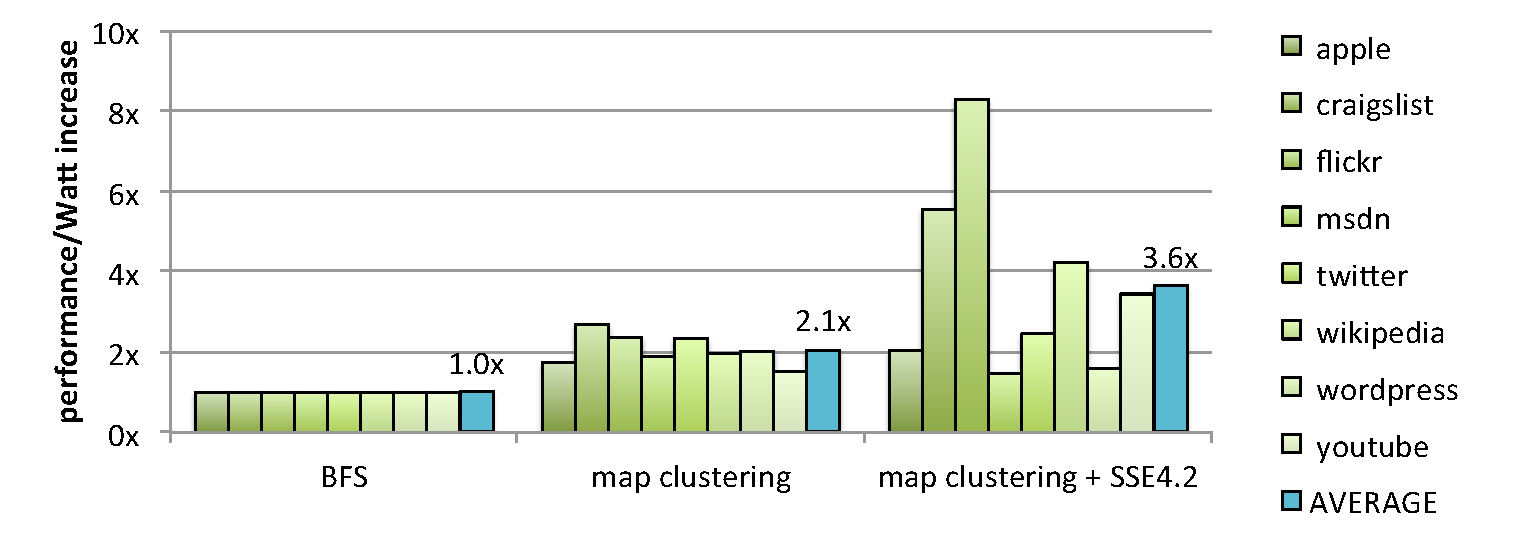
\includegraphics[trim=0 0 0 0,clip,width=1.0\columnwidth]{chapter6/csspower}
\caption{\textbf{Performance/Watt increase for clustered webpage layout.}}
\label{fig:csspower}
\end{figure}

\subsubsection{Power}
Much of our motivation for parallelization is better performance-per-Watt, so we evaluate power efficiency. To measure power, we sampled the power performance counters during layout. Each measurement looped over the same webpage over 1s due to the low resolution of the counter. Our setup introduces warm cache effects, but we argue it is still reasonable because a full layout engine would use multiple passes and therefore also have a warm cache across traversals.

In Figure~\ref{fig:csspower}, we show a 2.1X improvement in power efficiency for clustered sequential evaluation, which matches the 2.1X sequential speedup of Figure~\ref{fig:cssspeedup}. Likewise, we report a 3.6X cumulative improvement in power efficiency when vectorization is included, which is close to the 3.5X speedup. Thus, both in sequential and parallel contexts, clustering improves performance per Watt. Furthermore, it supports the general reasoning in parallel computing of 'race-to-halt' as a strategy for improving power efficiency.


\begin{figure}
\centering
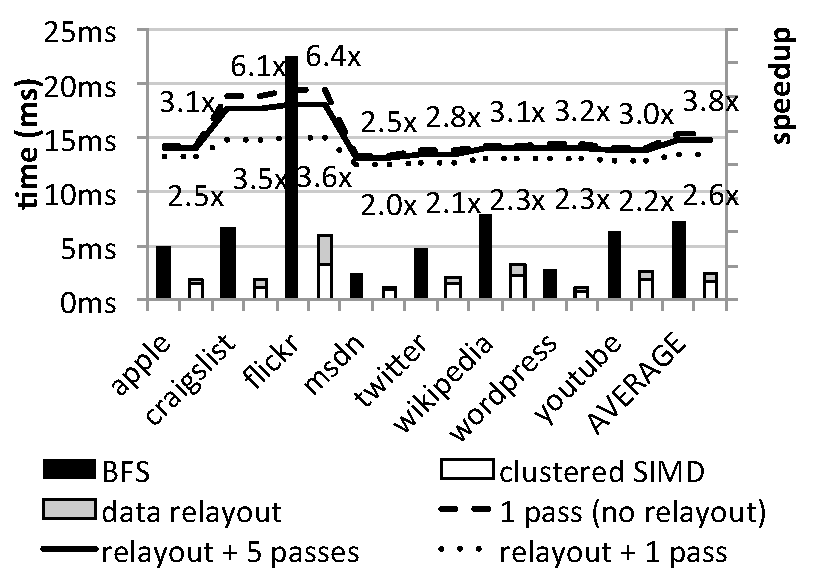
\includegraphics[trim=0 0 0 0,clip,width=0.6\columnwidth]{chapter6/datarelayouttime3}
\caption{\textbf{Impact of data relayout time on total CSS speedup.} Bars depict layout pass times. Speedup lines show the impact of including clustering preprocessing time.}
\label{fig:cssrelayout}
\end{figure}



\subsubsection{Overhead}
Our final examination of clustering is of the overhead. Time spent clustering before layout must not outweigh the performance benefit; it is an instance of the planning problem. 

For the case of data visualization, we convert the data structure into arrays with an offline preprocessor. Thus, our data visualizations experience no clustering cost.

For webpage layout, clustering is performed on the client when the webpage is received. We measured performing sequential two-pass clustering. Figure~\ref{fig:cssrelayout} shows the overhead relative to one pass using the bars. The highest relative overhead was for the Flickr homepage, where it reaches almost half the time of one pass. However, layout occurs in multiple passes. For a 5-pass layout engine where we model each pass as similar to the one we optimized, the overhead is amortized. The small gap between the solid and dashed lines in Figure~\ref{fig:cssrelayout} show there is little difference when we include the preprocessing overhead in the speedup calculation.



\section{Related Work}
\begin{enumerate}
\item representation The representation might be further compacted. For example, the last two arrays will have null values for Circle nodes. Even in the case of full utilization, space can be traded for time for even more aggressive compression [[CITE rinard]]
\item sims limit studies
\item duane
\item trishul
\item gnu irregular array stuff
\end{enumerate}
 %case studies
\chapter{Conclusion} %conclusion

\appendix
\chapter{Layout Grammars}

\printbibliography

\end{document}
